
\documentclass{article} % For LaTeX2e
\usepackage{iclr2026_conference,times}

% Optional math commands from https://github.com/goodfeli/dlbook_notation.
\input{math_commands.tex}

\usepackage{hyperref}
\hypersetup{colorlinks=true,linkcolor=blue,citecolor=blue,urlcolor=blue}
\usepackage{url}
\usepackage{amsmath,amssymb,amsthm}
\usepackage{algorithm}
\usepackage{algorithmic}
\usepackage{graphicx}
\usepackage{tikz}
\usetikzlibrary{calc}
\usepackage{booktabs}
\usepackage{subcaption}
\usepackage{enumitem}
\usepackage{bbm}

\newtheorem{theorem}{Theorem}
\newtheorem{lemma}[theorem]{Lemma}
\newtheorem{proposition}[theorem]{Proposition}
\newtheorem{corollary}[theorem]{Corollary}
\newtheorem{definition}{Definition}
\newtheorem{remark}{Remark}
\newtheorem{assumption}{Assumption}
\newtheorem{example}{Example}
\newtheorem*{theorem*}{Theorem}
\newtheorem*{lemma*}{Lemma}
\newtheorem*{proposition*}{Proposition}
\newtheorem*{corollary*}{Corollary}
\newtheorem*{remark*}{Remark}
\newcommand{\zz}[1]{\textcolor{blue}{(zz: #1)}}  
\newcommand{\hl}[1]{\textcolor{red}{#1}}  

\title{Beyond Best-of-Infinity:\\ Finite-Generation Limits of Test-Time LLM Ensembles}

% Authors must not appear in the submitted version. They should be hidden
% as long as the \iclrfinalcopy macro remains commented out below.
% Non-anonymous submissions will be rejected without review.

\author{Anonymous Authors}

% The \author macro works with any number of authors. There are two commands
% used to separate the names and addresses of multiple authors: \And and \AND.
%
% Using \And between authors leaves it to \LaTeX{} to determine where to break
% the lines. Using \AND forces a linebreak at that point. So, if \LaTeX{}
% puts 3 of 4 authors names on the first line, and the last on the second
% line, try using \AND instead of \And before the third author name.

\newcommand{\fix}{\marginpar{FIX}}
\newcommand{\new}{\marginpar{NEW}}
\providecommand{\R}{\mathbb{R}}
\providecommand{\E}{\mathbb{E}}
\providecommand{\argmax}{\mathop{\mathrm{arg\,max}}\limits}
\providecommand{\argmin}{\mathop{\mathrm{arg\,min}}\limits}
\providecommand{\D}{\mathcal{D}}
\providecommand{\Aq}{\mathcal{A}_q}
\providecommand{\simplex}{\Delta_K}
\providecommand{\Risk}{R}
\providecommand{\eRisk}{\widehat{R}}
\providecommand{\KL}{\mathrm{KL}}
\providecommand{\ip}[2]{\langle #1,\, #2\rangle}
\providecommand{\Qcal}{\mathcal{Q}}
\providecommand{\Pcal}{\mathcal{P}}
\providecommand{\Fcal}{\mathcal{F}}
\providecommand{\VC}{\mathrm{VC}}
\providecommand{\dhat}{\widehat{\delta}}
\providecommand{\phat}{\widehat{p}}
\providecommand{\Mhat}{\widehat{M}}
\providecommand{\what}{\widehat{w}}
\providecommand{\wstar}{w^{\star}}
\providecommand{\sign}{\mathrm{sign}}
\providecommand{\Too}{\widetilde{O}}
\providecommand{\boinf}{Best-of-$\infty$}
\providecommand{\boinflower}{best-of-$\infty$}

% Proof-status tags (author tracking).
% Master switch: set to \showstatustrue while drafting to display the tags,
% or \showstatusfalse before submission to hide ALL of them at once.
\newif\ifshowstatus
\showstatustrue   % <-- flip to \showstatusfalse for the submission version
\ifshowstatus
  \providecommand{\solid}{\textsc{[solid]}}
  \providecommand{\needsproof}{\textsc{[needs-proof]}}
  \providecommand{\conjecture}{\textsc{[conjecture]}}
\else
  \providecommand{\solid}{}
  \providecommand{\needsproof}{}
  \providecommand{\conjecture}{}
\fi

%\iclrfinalcopy % Uncomment for camera-ready version, but NOT for submission.
\begin{document}
\maketitle


\begin{abstract}
Weighting an ensemble of frozen large language models (the ``Best-of-$\infty$'' problem of \citet{komiyama2026best}) is, stripped of bespoke vocabulary, a sixty-year-old object: convex-combination aggregation of $K$ fixed probabilistic classifiers under $0/1$ loss, with problem-dependent answer sets. Under this loss the only surviving quantity is the scalar ensemble margin $M_q(w)$, so the hypothesis class is a family of margin-sign indicators of VC dimension $\tilde O(KA)$, and a textbook uniform-convergence argument already recovers the $1/\sqrt{Q}$ generalization behavior observed on benchmarks, with $Q$ the number of problems. Our central observation is that the LLM setting has a \emph{second} sample size absent from classical aggregation: each per-model answer distribution is itself estimated from $N$ generations, so the margins are noisy. We show that the excess risk of the fitted weights splits cleanly into a $Q$-term, driven by problem sampling, and an $N$-term, driven by margin-estimation noise; a single Tsybakov margin exponent $\beta$, the mass of problems whose true margin lies near zero, governs both. The $Q$-term is acceleratable to $(KA/Q)^{(\beta+1)/(\beta+2)}$, but the $N$-term is an \emph{irreducible floor} of order $N^{-\beta/2}$ that no amount of $Q$ can remove, because problems that are near-ties at sampling resolution $1/\sqrt N$ flip sign regardless of how many other problems are collected. The resulting joint $(N,Q)$ rate yields an explicit, LLM-specific rule for allocating a fixed test-time-compute budget between more problems and more generations. We are explicit about proof status throughout: the VC baseline and the sign-reliability lemma are fully proved; the accelerated $Q$-rate, the floor, and the joint rate are stated with proof sketches and named open gaps, and a minimax lower bound is posed as the load-bearing next step. Two synthetic multinomial simulations confirm that the two terms are genuinely distinct phenomena rather than relabelings, and we lay out an implementation-ready protocol for estimating $\beta$ and validating both rates on released benchmark generations.
\end{abstract}


\section{Introduction}
\label{sec:intro}

Suppose you have $K$ large language models, all frozen, and a benchmark of hard
problems. For each problem you sample many generations from each model, tally
how often each answer appears, and want to combine the models into one predictor
that answers as many problems correctly as possible. Two knobs control your cost.
You can collect more problems, enlarging the benchmark you fit on, or you can
sample more generations per model, sharpening your estimate of how each model
actually behaves on each problem. Given a fixed test-time-compute budget, how
should you split it between more problems and more generations? This is the
practical question behind the recently popularized ``Best-of-$\infty$'' ensemble
weighting problem of \citet{komiyama2026best}, and it is the question this paper
answers.

Our one-sentence thesis is that LLM ensemble weighting is convex-combination
aggregation of $K$ fixed probabilistic classifiers under $0/1$ loss, a
sixty-year-old object, but with a \emph{second} sample size, the number of
generations $N$, absent from classical aggregation theory, and this second
sample size sets an irreducible error floor of order $N^{-\beta/2}$ that no
number of problems can remove.

\paragraph{The reframing move.}
Once one writes the ensemble under $0/1$ loss, the machinery is completely
standard. There are $K$ language models, indexed $i=1,\dots,K$.
\begin{equation}
\label{eq:intro-K}
i \in \{1,\dots,K\}.
\end{equation}
Problems $q$ are drawn i.i.d.\ from an unknown distribution $\D$, and a benchmark
is $Q$ such draws.
\begin{equation}
\label{eq:intro-Q}
q \sim \D, \qquad q_1,\dots,q_Q \overset{\text{i.i.d.}}{\sim} \D.
\end{equation}
Each problem $q$ carries a finite answer set $\Aq$ with a gold answer
$a_q^\star \in \Aq$, and each model $i$ has a true answer distribution
$p_i(\cdot\mid q)$ that we estimate by the empirical frequency $\phat_i(\cdot\mid q)$
over $N$ generations. For any wrong answer $a\ne a_q^\star$, the score gap between
gold and $a$, coordinate by model, is
\begin{equation}
\label{eq:intro-delta}
(\delta_{q,a})_i = p_i(a_q^\star\mid q) - p_i(a\mid q) \in [-1,1].
\end{equation}
Weighting the models by $w$ in the simplex $\simplex$ and asking whether the
mixture puts more mass on the gold answer than on every wrong answer, the only
quantity that survives under $0/1$ loss is the scalar ensemble margin
\begin{equation}
\label{eq:intro-margin}
M_q(w) = \min_{a\ne a_q^\star} \ip{w}{\delta_{q,a}}
        = \min_{a\ne a_q^\star} \sum_{i=1}^K w_i\big(p_i(a_q^\star\mid q)-p_i(a\mid q)\big).
\end{equation}
The ensemble is correct on $q$ exactly when $M_q(w)>0$. This is a linear opinion
pool \citep{stone1961opinionpool,genest1986combining}, learned by stacking
\citep{wolpert1992stacked,breiman1996stacked}, in the language of forecast
combination \citep{bates1969combination} and weighted majority
\citep{littlestone1994weighted}, and it is not boosting, which builds weak
learners adaptively, nor bagging one base learner. It is the frozen-expert,
late-fusion regime.

\paragraph{A small worked example.}
Take $K=2$ models and one problem with a single wrong answer, so $M_q(w)$ is a
single inner product and the correctness region in the simplex is a halfspace.
\begin{equation}
\label{eq:intro-K2}
M_q(w) = \ip{w}{\delta_q}, \qquad \text{correct} \iff \ip{w}{\delta_q}>0.
\end{equation}
If $\delta_q = (0.4,-0.1)$ and $w=(0.5,0.5)$, then $M_q(w)=0.15>0$: the ensemble
is correct. Model~1 strongly prefers the gold answer, model~2 slightly prefers
the wrong one, and equal weighting still lands correct with a comfortable margin.
When the margin is instead a min over several wrong answers, the correctness
region is an intersection of halfspaces, a polytope, but the object is the same.

\paragraph{The gap classical aggregation misses.}
In sixty years of aggregation theory the expert outputs $p_i(\cdot\mid q)$ are
taken as exact. In the LLM setting they are not: each $p_i(\cdot\mid q)$ is
estimated from $N$ generations, so the margins we optimize are noisy versions of
the true margins. This is the whole novelty. There are two independent sample
sizes. The number of problems $Q$ controls statistical generalization across
$\D$; the number of generations $N$ controls the reliability of the margins
themselves. Writing $\wstar = \argmin_w R(w)$ for the best population weights,
$\what$ for the weights fit on empirical margins, and $R_N(w) = \Pr_q[\Mhat_q(w)\le 0]$
for the empirical-margin risk, the excess risk splits cleanly into three terms,
\begin{equation}
\label{eq:intro-decomp}
R(\what)-R(\wstar)
= \underbrace{\big[R(\what)-R_N(\what)\big]}_{\text{(i) }N}
+ \underbrace{\big[R_N(\what)-R_N(\wstar)\big]}_{\text{(ii) }Q}
+ \underbrace{\big[R_N(\wstar)-R(\wstar)\big]}_{\text{(iii) }N},
\end{equation}
where terms (i) and (iii) live in the $N$-term of margin-estimation noise and
term (ii) is the classical $Q$-term of problem sampling. A single geometric
quantity governs both terms: the Tsybakov margin exponent $\beta$, the mass of
problems whose true margin sits near zero,
\begin{equation}
\label{eq:intro-margincond}
\Pr_{q\sim\D}\big[\,0<|M_q(\wstar)|\le t\,\big] \le C\,t^{\beta}, \qquad t>0.
\end{equation}

\paragraph{The joint rate.}
The $Q$-term is the well-studied one: under \eqref{eq:intro-margincond} the
low-noise fast-rate machinery of \citet{mammen1999smooth,tsybakov2004optimal}
accelerates it from $\sqrt{KA/Q}$ toward $KA/Q$, where $A=\max_q|\Aq|$. The
$N$-term is the new content. A problem whose true margin is within $1/\sqrt N$
of zero is a coin flip at sampling resolution, so it flips sign regardless of how
many other problems are collected; the fraction of such problems is exactly
$N^{-\beta/2}$ under \eqref{eq:intro-margincond}. Assembling the two terms
gives the boxed joint rate,
\begin{equation}
\label{eq:intro-joint}
\boxed{\;
R(\what)-R(\wstar) \;\lesssim\;
\underbrace{\Big(\tfrac{KA}{Q}\Big)^{\frac{\beta+1}{\beta+2}}}_{\text{more problems}}
\;+\;
\underbrace{C\,N^{-\beta/2}}_{\text{more generations}}\; }
\end{equation}
in which the \emph{same} exponent $\beta$ sets both how fast the weights are
learned and how hard the irreducible floor bites. Minimizing
\eqref{eq:intro-joint} subject to a fixed budget $NQK=B$ yields an explicit,
LLM-specific rule for allocating test-time compute between problems and
generations, an actionable deliverable that no classical aggregation paper can
state, precisely because classical aggregation has no $N$. This places the work
squarely in the test-time-compute literature
\citep{brown2024largelm,snell2025scalinglt,wu2024inferencesl,wang2022selfconsistencyic},
but with a statistical rather than heuristic answer to how compute should be spent.

\paragraph{Contributions.}
The contributions are facets of the single idea that the ensemble has two sample
sizes governed by one margin exponent. First, we make the reframing precise: the
hypothesis class of margin-sign indicators has VC dimension $\tilde O(KA)$, and a
textbook uniform-convergence bound (our Theorem~\ref{thm:main} warm-up) already
recovers the $1/\sqrt Q$ generalization behavior observed on benchmarks; this part
is an honest, sharpened restatement of \citet{komiyama2026best}, not new theory.
Second, and centrally, we introduce the second sample size $N$ and prove the
two-term decomposition \eqref{eq:intro-decomp}, with a margin sign-reliability
lemma (Lemma~\ref{lem:1}) driving the floor. Third, we state the accelerated
$Q$-rate (Proposition~\ref{prop:1}), the $N$-floor (Proposition~\ref{prop:2}), and
the joint rate (Theorem~\ref{thm:generalization}), and derive the budget-allocation
corollary from \eqref{eq:intro-joint}. Fourth, we pose the minimax lower bound
that would elevate the floor from an upper bound to an irreducibility statement as
the load-bearing next step (Theorem~\ref{thm:convergence}).

\paragraph{Honesty about status.}
We are explicit about the proof status of every claim. The VC baseline and the
sign-reliability lemma are proved in the appendix. The accelerated $Q$-rate, the floor, and the joint rate are stated
with proof sketches and named open gaps, chiefly transporting the Tsybakov
argument through the min-over-answers loss and coupling the noisy optimization of
$\what$ into term (i), and the minimax lower bound is posed, not proved. On the
empirical side, two synthetic multinomial simulations are completed and reported
in Section~\ref{sec:experiments}: one confirms that sign flips are confined to the
$|M_q|\lesssim 1/\sqrt N$ band and that band mass decays like $N^{-\beta/2}$, and
one exhibits a winner's-curse optimization bias at fixed $Q$ that decays like
$1/\sqrt N$. Together they establish that the two terms are genuinely distinct
phenomena, not relabelings of one. Real-benchmark validation, estimating $\beta$
per benchmark from released generations and fitting both rates, is
implementation-ready on the released data but not yet run, and we present it as a
concrete protocol rather than a completed result.

\paragraph{Outline.}
Section~\ref{sec:related} places the work relative to fixed-classifier aggregation,
low-noise fast-rate theory, PAC-Bayes, and LLM ensembling.
Section~\ref{sec:background} fixes notation and states the classifier-aggregation
reduction. Section~\ref{sec:method} develops the warm-up VC bound and then the core
two-term decomposition and its two rates. Section~\ref{sec:theory} collects the
formal statements (the margin condition, the accelerated $Q$-rate, the $N$-floor,
the joint rate, the budget corollary, and the posed lower bound) with proof
sketches; full proofs are in Appendix~\ref{app:proofs-uc}.
Section~\ref{sec:experiments} reports the two synthetic term-isolation
simulations and lays out the implementation-ready benchmark protocol, with an
explicit theorem-to-experiment map. Section~\ref{sec:conclusion} states the
open gaps and the practical takeaway (estimate $\beta$ first, then allocate
compute), and Section~\ref{sec:conclusion} concludes.


\section{Related Work}
\label{sec:related}

Our thesis is that LLM ensemble weighting is convex-combination aggregation of
$K$ frozen soft classifiers under $0/1$ loss, and that its only genuinely new
statistical feature is a \emph{second} sample size $N$. We position the work
against four literatures: fixed-classifier aggregation, low-noise fast-rate
theory, PAC-Bayes, and LLM ensembling / test-time compute.

\paragraph{Fixed-classifier aggregation and late fusion.}
The mixture score the ensemble evaluates is a linear opinion pool of expert
distributions,
\begin{equation}
\label{eq:rw-pool}
S_w(a\mid q) = \sum_{i=1}^K w_i\, p_i(a\mid q), \qquad w\in\simplex,
\end{equation}
and $M_q(w)$ in \eqref{eq:intro-margin} is exactly the margin of the
$\argmax_a S_w(a\mid q)$ rule. Aggregating fixed experts by a convex combination
of their probability vectors is the linear opinion pool of
\citet{stone1961opinionpool,genest1986combining}, learned on held-out data it is
stacking \citep{wolpert1992stacked,breiman1996stacked}, in econometrics it is
forecast combination \citep{bates1969combination}, and when each expert is
collapsed to its top answer it is weighted majority
\citep{littlestone1994weighted}. Every one of these takes the expert outputs
$p_i(\cdot\mid q)$ as exact: the theory is written as if $N=\infty$. This is
precisely the regime our $N$-term escapes. The setting is also distinct from
ensemble methods that construct or perturb base learners: boosting builds weak
learners adaptively \citep{schapire1997boostingtm,freund1997adg} and bagging
resamples the data of a single learner \citep{breiman1996baggingp}, whereas here
the $K$ LLMs are frozen and given. Our contribution relative to this literature
is not the aggregation object but the observation that its inputs are themselves
$N$-sample estimates, which injects a second, irreducible error source absent
from all prior fixed-expert analyses.

\paragraph{Low-noise fast rates.}
The $Q$-term term (ii) of the decomposition \eqref{eq:intro-decomp} is
classical excess risk for a fixed loss over the margin-sign class $\Fcal$, and its
acceleration under the margin condition \eqref{eq:intro-margincond} is the
Mammen--Tsybakov low-noise phenomenon
\citep{mammen1999smooth,tsybakov2004optimal,tsybakov2009introduction}. The rate
in Proposition~\ref{prop:1} is obtained by the standard local-Rademacher and
peeling machinery
\citep{bartlett2005local,koltchinskii2006local,massart2006risk,bartlett2002rademacher,koltchinskii2001furthereo,audibert2005fastlr},
and the underlying capacity count uses VC/shattering arguments
\citep{vapnik1971uniform,sauer1972density,shelah1972combinatorial,blumer1989learnability}
together with the arrangement-cell view of intersecting halfspaces
\citep{zaslavsky1975facing}. We import these tools rather than extend them; the
honest statement is that we apply Tsybakov's fast-rate framework to the LLM
aggregation class, with the two transport subtleties (the min-over-answers loss
and the $N$-perturbed objective) flagged in Section~\ref{sec:theory}. What is new
is that the \emph{same} margin exponent $\beta$ appearing in these fast rates also
governs the $N$-floor $N^{-\beta/2}$ through the elementary sign-reliability bound
of Lemma~\ref{lem:1} \citep{hoeffding1963probability}. The fast-rate literature
has one sample size; we show a single $\beta$ ties the two here.

\paragraph{PAC-Bayes.}
The alternative certificate route, PAC-Bayes
\citep{mcallester1999pacbayes,dziugaite2017computing}, replaces the class-wide VC
capacity by the divergence of the learned posterior from a data-free prior. In our
setting it is an optional tightening of the $Q$-term certificate, not
load-bearing, and it carries two well-known caveats: the Gibbs-to-deterministic
conversion costs a factor via C-bound / Chebyshev--Cantelli arguments
\citep{viallard2021selfboundingmv,wu2021chebyshevcantellipi}, and a uniform-weight
posterior with zero KL can certify a comparable bound, so a favorable number may
reflect the class rather than the learner. We therefore demote PAC-Bayes to a
remark and an appendix ablation, keeping the two-term decomposition as the
central object.

\paragraph{LLM ensembling and test-time compute.}
The closest work is \citet{komiyama2026best}, whose Best-of-$\infty$ weighting we
reframe: their adaptive-stopping procedure targets the $N$-floor and their MILP
weighting targets the $Q$-term, and the decomposition \eqref{eq:intro-decomp}
shows these are the two summands of one excess-risk bound. Other ensembling
schemes, mixture-of-agents \citep{wang2024mixtureofagentsel} and pairwise
ranking fusion \citep{jiang2023llmblenderel}, operate in the same frozen-expert
regime but offer no $(N,Q)$ statistics. On the test-time-compute side, scaling
generations, verification, and self-consistency
\citep{brown2024largelm,snell2025scalinglt,wu2024inferencesl,wang2022selfconsistencyic,gao2022scalinglf,cobbe2021trainingvt,chen2024provablesl,aggarwal2023letsss}
studies how to spend inference budget, but treats problems and generations
heuristically; the budget-allocation corollary derived from
\eqref{eq:intro-joint} gives a statistical rule for splitting a fixed budget
$NQK=B$ between more problems and more generations. Our empirical validation uses
released benchmark generations, AIME, GPQA-D \citep{rein2023gpqaag}, and MATH500
\citep{hendrycks2021measuringmp}, for the planned per-benchmark $\beta$
estimation described in Section~\ref{sec:experiments}.

\paragraph{The gap.}
No prior work introduces the second sample size $N$ or the resulting $N$-floor.
Classical aggregation assumes exact experts, fast-rate theory assumes one sample
size, and the LLM-ensembling literature treats generations heuristically. The
load-bearing novelty here is exactly the two-term decomposition and the
$\beta$-governed floor.


\section{Method}
\label{sec:method}

\subsection{Notation}
\label{sec:method-notation}
There are $K$ language models, indexed by $i=1,\dots,K$. Problems are drawn
i.i.d.\ from an unknown distribution $\D$, and a benchmark is a finite sample
$q_1,\dots,q_Q \overset{\text{i.i.d.}}{\sim} \D$. Each problem $q$ carries a
finite answer set $\Aq$ and a gold answer $a_q^\star \in \Aq$. Model $i$ has a
true answer distribution $p_i(\cdot\mid q)$ over $\Aq$, where $p_i(a\mid q)$ is
the probability that a single generation of model $i$ on problem $q$ returns
answer $a$. We do not observe $p_i(\cdot\mid q)$ directly; instead we draw $N$
independent generations from model $i$ and estimate it by the empirical frequency
of each answer,
\begin{equation}
\label{eq:phat}
\phat_i(a\mid q) = \frac1N\sum_{n=1}^N \mathbf 1[\text{generation }n\text{ is }a],
\end{equation}
so $\phat_i(a\mid q)$ is simply the fraction of the $N$ samples equal to $a$
(a running tally, or ``vote count,'' normalized by $N$). Both $p_i(\cdot\mid q)$
and $\phat_i(\cdot\mid q)$ live in the probability simplex
$\Delta_{|\Aq|}=\{v\in\R^{|\Aq|}:v_a\ge 0,\ \sum_a v_a=1\}$ over the answer set,
i.e.\ each is a nonnegative vector of length $|\Aq|$ summing to one (one
probability per candidate answer). By the law of large numbers
$\phat_i(\cdot\mid q)\to p_i(\cdot\mid q)$ as $N\to\infty$, with sampling error of
order $1/\sqrt N$; this $N$ is the second sample size that drives the $N$-term
studied below.

The ensemble combines the models with a convex weight vector
$w \in \simplex = \{w\in\R^K : w_i\ge 0,\ \sum_i w_i = 1\}$. It scores each answer
by the weighted average of the models' probabilities,
\begin{equation}
\label{eq:score}
S_w(a\mid q) = \sum_{i=1}^K w_i\, p_i(a\mid q),
\end{equation}
a \emph{linear opinion pool} of the $K$ experts (again a distribution over $\Aq$,
since the $w_i$ sum to one), and predicts the highest-scoring answer,
\begin{equation}
\label{eq:predictor-notation}
f_w(q) = \argmax_{a\in\Aq} S_w(a\mid q).
\end{equation}
This is exactly \emph{weighted majority voting} in the large-sample limit: as
$N\to\infty$, drawing generations from model $i$ with probability $w_i$ and
taking the most frequent answer converges to $\argmax_a S_w(a\mid q)$. Equal
weights $w_i=1/K$ recover ordinary (unweighted) majority voting across models; the
contribution of this paper is that a well-chosen $w$ beats the uniform pool, and
Section~\ref{sec:method-milp} shows how to find it. At finite $N$ we substitute
the estimates $\phat_i$ for $p_i$, which is the only source of the $N$-term.

Under $0/1$ loss the only surviving quantity is a scalar margin. For a wrong
answer $a\ne a_q^\star$, the score gap collects how much more probability each
model places on the gold answer than on $a$,
\begin{equation}
\label{eq:delta}
\delta_{q,a}\in\R^K,
\qquad
(\delta_{q,a})_i = p_i(a_q^\star\mid q) - p_i(a\mid q) \in [-1,1].
\end{equation}
For each wrong answer $a$, the signed gap $\ip{w}{\delta_{q,a}}$ measures how
much more mixture mass sits on the gold answer than on $a$: it is positive when
the ensemble beats $a$ and negative when $a$ wins. The ensemble margin is the
gap against the \emph{hardest} contender, i.e.\ the minimum of these gaps over
all wrong answers,
\begin{equation}
\label{eq:M}
M_q(w) = \min_{a\ne a_q^\star}\ \ip{w}{\delta_{q,a}}.
\end{equation}
Taking the minimum is the conservative choice: the ensemble is correct only if
it beats \emph{every} wrong answer, so $M_q(w)>0$ (all gaps positive) means
correct, while $M_q(w)\le 0$ (some contender ties or wins) means wrong. The empirical margin of $p$ is defined as $\phat$,
\begin{equation}
\label{eq:Mhat}
\Mhat_q(w) = \min_{a\ne a_q^\star}\ \ip{w}{\dhat_{q,a}},
\qquad
(\dhat_{q,a})_i = \phat_i(a_q^\star\mid q) - \phat_i(a\mid q).
\end{equation}

\paragraph{Example.}
Take $K=2$ models, one problem $q$ with $|\Aq|=3$, so two wrong answers
$a_1,a_2$. Suppose
\begin{equation}
\label{eq:wex1}
\delta_{q,a_1} = (0.4,\,-0.1),\quad
\delta_{q,a_2} = (0.1,\,0.3),\quad
w = (0.5,\,0.5).
\end{equation}
Then $\ip{w}{\delta_{q,a_1}} = 0.15$ and $\ip{w}{\delta_{q,a_2}} = 0.20$, so
$M_q(w) = \min(0.15,0.20) = 0.15 > 0$: the ensemble is correct, and the binding
constraint is the closer contender $a_1$.
\subsection{Algorithm}
\label{sec:method-framing}

At prediction time the ensemble runs weighted majority voting: for each problem
it draws $N$ generations per model, forms the empirical answer frequencies
$\phat_i(\cdot\mid q)$ of \eqref{eq:phat}, scores each answer by the pooled
estimate $\widehat S_w(a\mid q)=\sum_i w_i\,\phat_i(a\mid q)$, and returns the
top-scoring answer (equivalently, the weighted plurality vote). As $N\to\infty$
this converges to the population predictor
$f_w(q)=\argmax_{a\in\Aq} S_w(a\mid q)$ of \eqref{eq:predictor-notation}.
Algorithm~\ref{alg:ensemble} states the full procedure: sample generations and
estimate each model's answer distribution, learn the weights $w$ by minimizing
the empirical $0/1$ risk over the simplex (Section~\ref{sec:method-milp}), then
predict by weighted majority vote. The population and empirical $0/1$ risks are
\begin{equation}
\label{eq:R}
\Risk(w) = \Pr_{q\sim\D}\!\big[M_q(w)\le 0\big],
\end{equation}
\begin{equation}
\label{eq:Rhat}
\eRisk(w) = \frac1Q\sum_{q=1}^Q \mathbf 1\!\big[\Mhat_q(w)\le 0\big].
\end{equation}


\begin{algorithm}[t]
\caption{Convex-weighted ensemble by majority voting}
\label{alg:ensemble}
\begin{algorithmic}[1]
\STATE \textbf{Input:} models $1,\dots,K$; benchmark $q_1,\dots,q_Q$; generations per model $N$
\FOR{each problem $q$ and model $i$}
  \STATE draw $N$ i.i.d.\ generations from model $i$ on problem $q$
  \STATE $\phat_i(a\mid q) \leftarrow \tfrac1N\sum_{n=1}^N \mathbf 1[\text{generation }n\text{ is }a]$ \hfill\COMMENT{empirical answer frequencies / vote counts, Eq.~\eqref{eq:phat}}
\ENDFOR
\STATE $\hat w \leftarrow \argmin_{w\in\simplex}\ \eRisk(w)$ \hfill\COMMENT{learn weights via the MILP of Section~\ref{sec:method-milp}}
\STATE \textbf{return} predictor $f_{\hat w}(q)=\argmax_{a\in\Aq}\sum_i \hat w_i\,\phat_i(a\mid q)$ \hfill\COMMENT{weighted majority vote}
\end{algorithmic}
\end{algorithm}

This is aggregation of $K$ fixed probabilistic classifiers under $0/1$ loss over
the convex-combination class, except that the label set $\Aq$ changes from
problem to problem. Table~\ref{tab:dictionary} maps each classification object to
its ensemble counterpart.

\begin{table}[t]
\centering
\caption{Analogy between classification and LLM ensembling.}
\label{tab:dictionary}
\begin{tabular}{ll}
\toprule
Classification & LLM ensemble \\
\midrule
feature $x$ & problem $q$ \\
label $y$ & answer $a$ \\
fixed soft classifier $h_i(x)\approx P(y\mid x)$ & model distribution $p_i(\cdot\mid q)$ \\
aggregated score $\sum_i w_i h_i(x)$ & mixture score $\sum_i w_i\,p_i(\cdot\mid q)$ \\
prediction $\argmax_y \sum_i w_i h_i(x)_y$ & $f_w(q)$ in \eqref{eq:predictor-notation} \\
empirical $0/1$ risk & $\eRisk(w)$ in \eqref{eq:Rhat} \\
\bottomrule
\end{tabular}
\end{table}

\subsection{Solving for the optimal weights: a MILP formulation}
\label{sec:method-milp}

The weight-learning step in Algorithm~\ref{alg:ensemble} (line~4) minimizes the
empirical $0/1$ risk over the simplex, but the objective is not concave, so
gradient methods need not find the optimum. We adopt the tractable
mixed-integer linear programming (MILP) formulation of \citet{komiyama2026best},
reproduced here, which solves the weight-optimization problem exactly at typical
scale.

\medskip
\noindent\emph{[The following is adapted verbatim from
\citet{komiyama2026best}; notation is reconciled with ours in the next
revision.]}

\paragraph{Setup.} Let $i \in \mathcal{K}$ index the LLMs, and let
$w = (w_1,\dots,w_K)$ be the weight vector with $w_i \ge 0$ and
$\sum_{i \in \mathcal{K}} w_i = 1$. Let $q \in \mathcal{Q}$ be the problem, with
answer domain $\mathcal{A}_q$ and gold answer $g_q \in \mathcal{A}_q$. In the
large-sample limit the ensemble answer for problem $q$ is deterministic,
\[
a_q = \argmax_j \Big\{ \sum_{i \in \mathcal{K}} w_i\, p_{i,j}^q \Big\},
\]
and the objective is the number of correct answers
$f(w) = \sum_{q \in \mathcal{Q}} \mathbf{1}[a_q = g_q]$.

\paragraph{Non-concavity.} $f(w)$ is a non-concave function on the simplex of
$w$. (Consider one question with two LLMs, one correct and one wrong: then
$f((1,0))=1$ and $f((0,1))=0$, yet the value dips below the chord in between.)
Although non-concavity rules out gradient-based optimality, a combinatorial
approach is tractable at typical scale, because the summand takes value one
within a polytope.

\begin{lemma}[Polytope lemma]
\label{lem:polytope}
Let $\{p_{ij}^q\}_{i\in[K],\,j\in\mathcal{A}_q}$ be arbitrary answer
distributions. Then the set on which answer $j$ is the most frequent,
\begin{equation}
\label{eq:nbest}
\Big\{ w \in \Delta_K:\ \sum_i w_i p_{ij}^q > \max_{j'\ne j} \sum_i w_i p_{ij'}^q \Big\},
\end{equation}
is a polytope.
\end{lemma}
\begin{proof}
The region \eqref{eq:nbest} is an intersection of the half-spaces
$\{w:\sum_i w_i p_{ij}^q > \sum_i w_i p_{ij'}^q\}$ over all $j'\ne j$, hence a
polyhedron; intersected with the simplex $\Delta_{\mathcal{A}_q}$ it is bounded,
hence a polytope.
\end{proof}

Maximizing the number of correct answers is thus equivalent to maximizing the
number of polytopes containing $w$. Introducing a binary variable $y_q$
indicating correctness of problem $q$, this becomes a MILP.

\begin{lemma}[MILP formulation]
\label{lem:milp}
Maximizing $f(w)$ is equivalent to the mixed-integer linear program
\begin{align}
\max_{w \in \Delta^K,\ y \in \{0,1\}^{|\mathcal{Q}|}} \quad & \sum_q y_q \\
\mathrm{s.t.}\quad & w_i \ge 0 \quad \forall i, \\
& \textstyle\sum_i w_i = 1, \\
& A_q w \ge -m\,(1 - y_q) \quad \forall q, \label{eq:milp-constraint}
\end{align}
where $A_q \in \mathbb{R}^{|\mathcal{A}_q|\times K}$ has $(j,i)$ entry
$p_{i,g_q}^q - p_{i,j}^q$ (row $j$ encodes that the gold answer $g_q$ outweighs
wrong answer $j$), and $m>0$ is chosen large enough that $A_q w \ge -m$ is
non-binding when $A_q w$ has a negative component.
\end{lemma}

The instance size grows with the number of LLMs $K$, the number of problems, and
the answer-set sizes $|\mathcal{A}_q|$. General MILP solving is NP-hard, but in
practice open-source solvers scale smoothly to $K \approx 10^1$ LLMs and
$\approx 10^3$ problems with $|\mathcal{A}_q| \approx 10^1$.

\paragraph{Max-margin solution.} The objective $f(w)$ has a continuous region of
optimal solutions; while any interior point is optimal in the limit, its
finite-$N$ behavior varies. We adopt the \emph{max-margin} solution, the most
interior point: introduce a margin $\xi>0$, replace $A_q w$ in
\eqref{eq:milp-constraint} with $A_q w - \xi$, and take the supremum of $\xi$ for
which the objective $\sum_q y_q$ does not decrease. This supremum is found by a
binary search over $\xi \in [0,m]$ of a monotone objective, which is practically
feasible.




\section{Theoretical Analysis}

Because we measure performance by $0/1$ loss, the only thing about $w$ that
matters on a problem is whether the margin is positive or not, so the natural
hypothesis class is the collection of margin-sign rules indexed by the simplex:
\begin{equation}
\label{eq:Fclass}
\Fcal = \big\{\, q\mapsto \mathbf 1[M_q(w)\le 0] : w\in\simplex \,\big\}.
\end{equation}
Each $w$ picks out the set of problems it gets wrong, and the indicator is the
$0/1$ error of that rule. It is worth seeing what the correct-region of weights
looks like, because its geometry is what the capacity bounds measure.

Consider first a problem with exactly two candidate answers, the gold answer and
one wrong answer. Then the margin is a single inner product $M_q(w)=\ip{w}{\delta_q}$,
which is linear in $w$, and the ensemble is correct precisely when this is
positive. The set $\{w:\ip{w}{\delta_q}>0\}$ is a \emph{halfspace}: the weights on
one side of the hyperplane $\ip{w}{\delta_q}=0$,
$
\{w : M_q(w)>0\} = \{w : \ip{w}{\delta_q}>0\}\ \text{(a halfspace).}$
In general a problem has $A_q:=|\Aq|$ candidate answers, one of which is gold, so
there are $m=A_q-1$ wrong answers, one gap $\ip{w}{\delta_{q,a}}$ per wrong
answer. The ensemble beats \emph{all} of them iff the smallest gap is positive,
so the margin is the pointwise minimum of $m$ linear functions,
$M_q(w)=\min_{a\ne a_q^\star}\ip{w}{\delta_{q,a}}$. A linear function $g(w)=\ip{w}{\delta}$ is concave (indeed affine): for any $w,w'$ and $\lambda\in[0,1]$,
by bilinearity of the inner product,
$
g\big(\lambda w+(1-\lambda)w'\big)
= \ip{\lambda w+(1-\lambda)w'}{\delta}
= \lambda\ip{w}{\delta} + (1-\lambda)\ip{w'}{\delta}
= \lambda\, g(w) + (1-\lambda)\, g(w')$. The pointwise minimum of concave functions is again concave, so $M_q$,
a minimum of the linear maps $w\mapsto\ip{w}{\delta_{q,a}}$, is concave in $w$.
Concavity is unrelated to the sign
threshold $M_q(w)>0$ that defines correctness. The correct-region is the set of
$w$ satisfying all $m$ inequalities at once, an intersection of $m$ halfspaces,
i.e.\ a \emph{polytope} (a region cut out by finitely many linear inequalities):
\begin{equation}
\label{eq:polytope}
\{w : M_q(w)>0\} = \bigcap_{a\ne a_q^\star}\{w : \ip{w}{\delta_{q,a}}>0\}.
\end{equation}
Figure~\ref{fig:simplex} illustrates both cases on the weight simplex for $K=4$,
where the simplex is a solid tetrahedron with vertices $e_1,\dots,e_4$.

\begin{figure}[t]
\centering
% Shared tetrahedron vertices (2D projection of the K=4 simplex).
% e_4 is the apex; e_3 is the back vertex (its edges are drawn dashed/hidden).
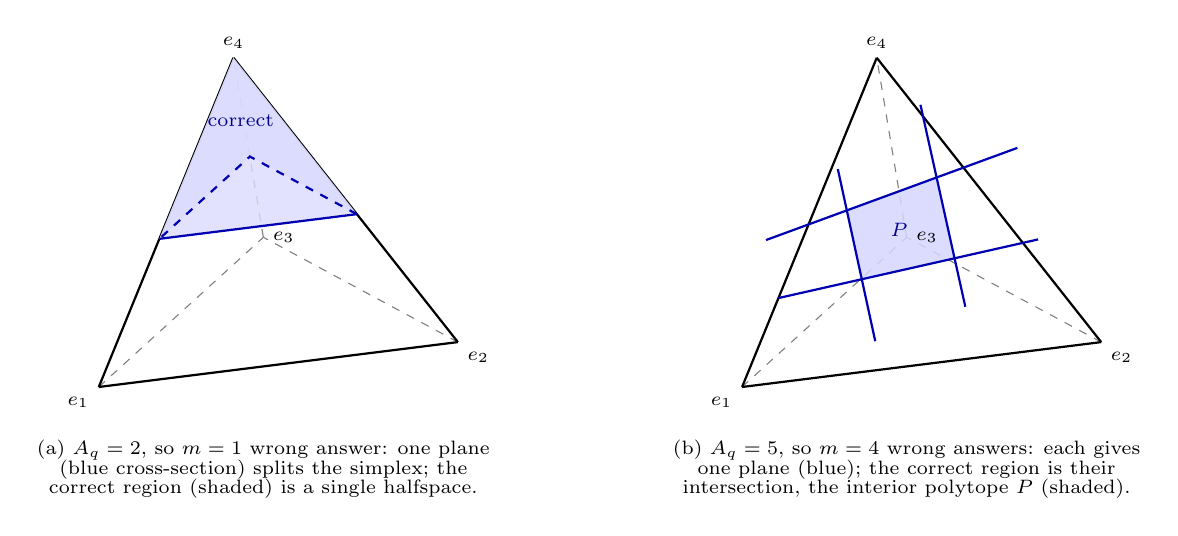
\begin{tikzpicture}[scale=1.9,
    every node/.style={font=\scriptsize}]
  % Panel (a): one wrong answer -> one halfspace
  \begin{scope}
    \coordinate (A) at (0,0);        % e_1
    \coordinate (B) at (2.4,0.3);    % e_2
    \coordinate (C) at (1.1,1.0);    % e_3 (back)
    \coordinate (D) at (0.9,2.2);    % e_4 (apex)
    % hidden edges to back vertex e_3
    \draw[gray,dashed] (A)--(C); \draw[gray,dashed] (B)--(C); \draw[gray,dashed] (C)--(D);
    % visible edges
    \draw[thick] (A)--(B) (A)--(D) (B)--(D);
    % cutting hyperplane {<w,delta>=0}: a triangular cross-section
    \coordinate (P1) at (0.405,0.99);   % on edge A--D
    \coordinate (P2) at (1.725,1.155);  % on edge B--D
    \coordinate (P3) at (1.01,1.54);    % on edge C--D
    % correct half (apex side) shaded
    \fill[blue!14,opacity=0.8] (P1)--(P2)--(D)--cycle;
    \fill[blue!14,opacity=0.8] (P1)--(P3)--(D)--cycle;
    \fill[blue!14,opacity=0.8] (P2)--(P3)--(D)--cycle;
    \draw[blue!70!black,thick] (P1)--(P2);
    \draw[blue!70!black,thick,dashed] (P2)--(P3)--(P1);
    \node[blue!55!black] at (0.95,1.78) {correct};
    \node[below left] at (A) {$e_1$};
    \node[below right] at (B) {$e_2$};
    \node[right] at (C) {$e_3$};
    \node[above] at (D) {$e_4$};
    \node[align=center] at (1.1,-0.55)
      {(a) $A_q=2$, so $m=1$ wrong answer: one plane\\[-1pt](blue cross-section) splits the simplex; the\\[-1pt]correct region (shaded) is a single halfspace.};
  \end{scope}
  % Panel (b): several wrong answers -> polytope
  \begin{scope}[xshift=4.3cm]
    \coordinate (A) at (0,0);
    \coordinate (B) at (2.4,0.3);
    \coordinate (C) at (1.1,1.0);
    \coordinate (D) at (0.9,2.2);
    \draw[gray,dashed] (A)--(C); \draw[gray,dashed] (B)--(C); \draw[gray,dashed] (C)--(D);
    \draw[thick] (A)--(B) (A)--(D) (B)--(D);
    % Four cutting planes; the shaded quadrilateral P below is EXACTLY the
    % intersection region, so each of its four edges lies on one blue line.
    \coordinate (Q1) at (0.80,0.72);
    \coordinate (Q2) at (1.42,0.86);
    \coordinate (Q3) at (1.30,1.40);
    \coordinate (Q4) at (0.70,1.18);
    % interior polytope P = intersection of the four halfspaces
    \fill[blue!16,opacity=0.85] (Q1)--(Q2)--(Q3)--(Q4)--cycle;
    % each blue line passes through two adjacent vertices of P and extends to the faces
    \draw[blue!70!black,thick] ($(Q1)!-0.9!(Q2)$)--($(Q2)!-0.9!(Q1)$); % edge Q1-Q2
    \draw[blue!70!black,thick] ($(Q2)!-0.6!(Q3)$)--($(Q3)!-0.9!(Q2)$); % edge Q2-Q3
    \draw[blue!70!black,thick] ($(Q3)!-0.9!(Q4)$)--($(Q4)!-0.9!(Q3)$); % edge Q3-Q4
    \draw[blue!70!black,thick] ($(Q4)!-0.6!(Q1)$)--($(Q1)!-0.9!(Q4)$); % edge Q4-Q1
    \node[blue!55!black] at (1.05,1.05) {$P$};
    \node[below left] at (A) {$e_1$};
    \node[below right] at (B) {$e_2$};
    \node[right] at (C) {$e_3$};
    \node[above] at (D) {$e_4$};
    \node[align=center] at (1.1,-0.55)
      {(b) $A_q=5$, so $m=4$ wrong answers: each gives\\[-1pt]one plane (blue); the correct region is their\\[-1pt]intersection, the interior polytope $P$ (shaded).};
  \end{scope}
\end{tikzpicture}
\caption{Correct-region of ensemble weights for a \emph{single} question $q$ with
$K=4$ models. The weight vector $w=(w_1,\dots,w_4)$ obeys $w_i\ge 0$ and
$w_1+w_2+w_3+w_4=1$, so it lives on the probability simplex; this constraint drops
one degree of freedom, turning the $4$-dimensional weights into a $3$-dimensional
solid \textbf{tetrahedron}. Its four \textbf{vertices} $e_1,\dots,e_4$ are the
pure weightings (vertex $e_i$ places all weight on model $i$); the black and
dashed lines are the tetrahedron's \emph{edges}, the boundary of the weight
domain.
Superimposed on this domain, each \textbf{blue line} is the trace of one decision
hyperplane $\{w:\ip{w}{\delta_{q,a}}=0\}$, one per wrong answer $a$, where the
ensemble is exactly tied with $a$, and the \textbf{shaded blue region} is the
correct-region $\{w:M_q(w)>0\}$, the weights that beat every wrong answer.
(a)~If the question has $A_q=2$ candidate answers there is $m=1$ wrong answer,
hence a single plane, and the correct-region is one halfspace (here $m$ blue
lines $=1$). (b)~If $A_q=5$ there are $m=4$ wrong answers, hence $4$ blue lines,
and the correct-region is the interior polytope $P$ where all four halfspaces
overlap.}
\label{fig:simplex}
\end{figure}
The maximum size of the answer set across questions is defined as
\begin{equation}
\label{eq:A}
A := \max_q |\Aq|.
\end{equation}

\subsection{A uniform-convergence baseline}
\label{sec:method-vc}

Fixing a problem, ``$M_q(w)\le 0$'' means $w$ lies outside an intersection of at
most $A-1$ homogeneous halfspaces in $\R^K$. A single halfspace-indicator class in
$\R^K$ has VC dimension $K$, and an intersection of $m$ of them has VC dimension
$O(Km\log m)$ by the Blumer composition bound \citep{blumer1989learnability}
(equivalently, the number of regions that $m$ hyperplanes cut $\R^K$ into is
polynomial in $m$, the classical hyperplane-arrangement count of
\citet{zaslavsky1975facing}). The \emph{capacity} of a hypothesis class is its VC
dimension, the largest number of problems the class can label in all possible
ways, a standard measure of how rich the class is and hence how much data uniform
convergence requires. Combining these gives
\begin{equation}
\label{eq:vc}
\VC(\Fcal) = \Too(KA),
\end{equation}
where $\Too(\cdot)$ is the usual $O(\cdot)$ up to logarithmic factors (here in $A$
and $Q$), which we suppress for readability. This yields the standard
uniform-convergence guarantee, our baseline.

\begin{theorem}[Uniform convergence over problems, \solid]%
\footnote{This theorem is fully proved in Appendix~\ref{app:proofs-gen}, as
opposed to results below that are stated with proof sketches or posed as open;
see the discussion of proof status in Section~\ref{sec:intro}.}
\label{thm:convergence}
There is a universal constant $c>0$ such that, with probability at least
$1-\delta$ over the $Q$ i.i.d.\ problems, simultaneously for all $w\in\simplex$,
\begin{equation}
\label{eq:thm1}
\big|\Risk(w)-\eRisk(w)\big|
\;\le\;
c\sqrt{\frac{KA\log A\,\log Q + \log(1/\delta)}{Q}}.
\end{equation}
\end{theorem}

\begin{proof}[Proof sketch]
Standard VC/Rademacher symmetrization with Sauer's lemma
\citep{sauer1972density,shelah1972combinatorial,vapnik1971uniform} applied to
$\Fcal$, using the capacity \eqref{eq:vc}. The $\log A$ and $\log Q$ factors are
the logarithmic overheads incurred when bounding the VC dimension of an
intersection of $A-1$ halfspaces (the $\log A$) and when passing from the growth
function to a uniform bound over $Q$ problems (the $\log Q$); these are exactly
the logarithmic terms absorbed into $\Too(\cdot)$ in \eqref{eq:vc}. Full argument
in Appendix~\ref{app:proofs-uc}.
\end{proof}

Inverting \eqref{eq:thm1} gives the sample-complexity reading
\begin{equation}
\label{eq:qneed}
Q \gtrsim \frac{KA}{\epsilon^2}\quad\text{for a gap}\le\epsilon,
\end{equation}
which is loose but correctly predicts the $1/\sqrt Q$ decay across benchmarks.
We record a PAC-Bayes tightening as an optional remark, not a headline
contribution; converting its randomized (Gibbs) guarantee to the deployed
deterministic weights relies on C-bound / Chebyshev--Cantelli arguments
\citep{viallard2021selfboundingmv,wu2021chebyshevcantellipi}.

% \begin{remark}[PAC-Bayes, demoted]
% \label{rem:pacbayes}
% Replacing the class-wide capacity by the divergence of a data-chosen posterior
% $\Qcal$ from a prior $\Pcal$ gives the McAllester bound on the Gibbs risk
% \citep{mcallester1999pacbayes},
% \begin{equation}
% \label{eq:mcallester}
% \E_{w\sim\Qcal}\Risk(w)
% \le
% \E_{w\sim\Qcal}\eRisk(w)
% + \sqrt{\frac{\KL(\Qcal\|\Pcal) + \log(2\sqrt Q/\delta)}{2(Q-1)}},
% \end{equation}
% minimized (for fixed $\Pcal$, $\lambda>0$) by the Gibbs posterior
% \begin{equation}
% \label{eq:gibbs}
% \Qcal^\star(w)\propto \Pcal(w)\,e^{-\lambda\eRisk(w)}.
% \end{equation}

% Two caveats keep this off the critical path: converting the Gibbs risk to the
% deployed deterministic $w$ costs a factor via C-bound/Chebyshev--Cantelli
% arguments \citep{viallard2021selfboundingmv,wu2021chebyshevcantellipi}, and a
% uniform posterior with $\KL(\Qcal\|\text{uniform})=0$ can certify a comparable
% bound, so a favorable number may reflect the class rather than the learner. We
% treat \eqref{eq:mcallester} as an appendix ablation.
% \end{remark}

\subsection{Decomposing the excess risk into a $Q$-term and an $N$-term}
\label{sec:method-decomp}

Let $\wstar$ be the best population weights and $\what$ the weights returned by
fitting the empirical margins (the Komiyama MILP \citep{komiyama2026best}, or any
surrogate),
\begin{equation}
\label{eq:wstar-what}
\wstar = \argmin_{w\in\simplex}\Risk(w),
\qquad
\what \in \argmin_{w\in\simplex}\eRisk(w).
\end{equation}
The weight-learning procedure in \eqref{eq:wstar-what} can only see empirical
margins, so the risk it can actually target lives at the empirical-margin level.
We define the empirical-margin risk, an expectation over both the problem draw
and the $N$ generations,
\begin{equation}
\label{eq:RN}
\Risk_N(w) := \Pr_{q,\,\text{gen}}\!\big[\Mhat_q(w)\le 0\big].
\end{equation}
The excess risk then splits into three pieces that isolate the two sample sizes,
\begin{equation}
\label{eq:decomp}
\Risk(\what) - \Risk(\wstar)
=
\underbrace{\big[\Risk(\what) - \Risk_N(\what)\big]}_{\text{(i) margin estimation, }N}
+ \underbrace{\big[\Risk_N(\what) - \Risk_N(\wstar)\big]}_{\text{(ii) problem sampling, }Q}
+ \underbrace{\big[\Risk_N(\wstar) - \Risk(\wstar)\big]}_{\text{(iii) margin estimation, }N}.
\end{equation}
Terms (i) and (iii) depend on the estimation noise from the $N$ generations, so
we group them as the \emph{$N$-term} (the error term driven by margin
estimation); term (ii) depends on the problem sample and is the \emph{$Q$-term}
(driven by problem sampling). This single identity is central to the paper:
everything below bounds these two terms and ties both to one exponent.

\paragraph{Worked example.}
Take $K=2$, $Q=3$ problems, weights $\wstar$, and true margins
$M_1(\wstar)=0.30,\ M_2(\wstar)=0.02,\ M_3(\wstar)=-0.25$, so $\Risk(\wstar)=1/3$
(problem $3$ wrong). At small $N$ the near-tie problem $q=2$ ($M_2=0.02$) can flip
sign in $\Mhat$; if it flips, $\Risk_N(\wstar)=2/3$, contributing $+1/3$ to term
(iii). The well-separated problems $q=1,3$ almost never flip. The gap between
$\Risk_N$ and $\Risk$ is thus driven entirely by mass near zero, the $N$-floor.

\subsection{The margin exponent and the two rates}
\label{sec:method-rates}

The baseline bound \eqref{eq:thm1} decays at the slow $1/\sqrt Q$ rate, which
holds for \emph{any} problem distribution and is therefore pessimistic: it
ignores that on most benchmarks the ensemble is not borderline on a typical
problem, but wins (or loses) by a comfortable margin. The problems that are
genuinely hard, for both learning the weights and estimating the margins from
$N$ generations, are the near-ties, those whose true margin $M_q(\wstar)$ sits
close to zero, because a small perturbation can flip them from correct to wrong.
Intuitively, then, the difficulty of the problem is controlled by \emph{how much
of the problem mass concentrates near the decision boundary} $M_q(\wstar)=0$. The
margin (Tsybakov) exponent $\beta$ makes this precise: a larger $\beta$ means
fewer near-tie problems, which we will show both accelerates the $Q$-term beyond
$1/\sqrt Q$ and sets the size of the irreducible $N$-floor. This is the source of
our faster, distribution-dependent rates below.

In the following, $\wstar$ is a fixed (deterministic) vector, the optimal weights
of \eqref{eq:wstar-what}, while the problem $q\sim\D$ is random; hence
$M_q(\wstar)$ is a scalar random variable, one real number per problem (its value
is the smallest of the $m=A_q-1$ gaps against the wrong answers). The probability
below is taken over the random draw of $q$.
\begin{definition}[Margin exponent $\beta$]
\label{def:tsybakov}
The problem distribution $\D$ has margin exponent $\beta\ge 0$ if there is a
constant $C>0$ with
\begin{equation}
\label{eq:margincond}
\Pr_{q\sim\D}\!\big[\,0 < |M_q(\wstar)| \le t\,\big] \le C\,t^{\beta}
\qquad \forall t>0.
\end{equation}
\end{definition}

\paragraph{Example.}
If the true margins $M_q(\wstar)$ are uniform on $[-1,1]$, then
$\Pr[|M_q|\le t] = t$, so $\beta=1$. If all margins are bounded away from zero,
say $|M_q(\wstar)|\ge m_0>0$ a.s., then \eqref{eq:margincond} holds for all
$\beta$, i.e.\ $\beta=\infty$: no near-ties, and both terms vanish fastest.

The $Q$-term is classical excess risk for the frozen loss over $\Fcal$; the
margin condition accelerates it in the Mammen--Tsybakov manner
\citep{mammen1999smooth,tsybakov2004optimal}.

\begin{proposition}[Accelerated $Q$-rate]
\label{prop:1}
Under \eqref{eq:margincond} with exponent $\beta$, the $Q$-term of
\eqref{eq:decomp} obeys
\begin{equation}
\label{eq:qrate}
\text{\emph{(ii)}} \;=\; \Too\!\left(\Big(\frac{KA}{Q}\Big)^{\frac{\beta+1}{\beta+2}}\right),
\end{equation}
interpolating between the slow rate $\sqrt{KA/Q}$ at $\beta=0$ and the fast rate
$KA/Q$ as $\beta\to\infty$.
\end{proposition}

\noindent This is a transport of Tsybakov's local-Rademacher/peeling framework
\citep{bartlett2005local,koltchinskii2006local,massart2006risk} to the class
$\Fcal$; the full argument is given in Appendix~\ref{app:proofs-gen}. Two
features of our setting make it non-standard.
First, recall that the ensemble predicts by $f_w(q)=\argmax_a S_w(a\mid q)$ with
the mixture score $S_w(a\mid q)=\sum_i w_i\,p_i(a\mid q)$ of
\eqref{eq:score}. The key observation is that the gap of a wrong answer $a$
is exactly the score of the gold answer $a_q^\star$ minus the score of $a$,
\begin{equation}
\label{eq:gap-is-score-diff}
\ip{w}{\delta_{q,a}}
= \sum_i w_i\big(p_i(a_q^\star\mid q)-p_i(a\mid q)\big)
= S_w(a_q^\star\mid q) - S_w(a\mid q),
\end{equation}
which is why we take the gap over wrong answers $a\ne a_q^\star$ only: it measures
how far $a_q^\star$'s score $S_w(a_q^\star\mid q)$ is \emph{above} the score
$S_w(a\mid q)$ of each competing answer, and comparing $a_q^\star$ with itself
gives the trivial gap $0$, so it is excluded. The ensemble's predicted answer is
the one with the highest score, $f_w(q)=\argmax_{a\in\Aq} S_w(a\mid q)$; we say
$a_q^\star$ ``wins'' when it is this $\argmax$, i.e.\ when the ensemble predicts
$a_q^\star$ and is therefore correct. By \eqref{eq:gap-is-score-diff}, $a_q^\star$
attains the highest score iff its score exceeds that of every wrong answer, i.e.\
iff every gap in \eqref{eq:gap-is-score-diff} is positive, i.e.\ iff
$M_q(w)=\min_{a\ne a_q^\star}\ip{w}{\delta_{q,a}}>0$. This is why $M_q(w)>0$ is
exactly the condition for a correct answer. The answer $a_q^\star$ does \emph{not}
automatically attain the highest score: if some wrong answer $a$ has
$S_w(a\mid q)>S_w(a_q^\star\mid q)$, then
$S_w(a_q^\star\mid q)-S_w(a\mid q)<0$, so that gap is negative and $M_q(w)<0$
(the ensemble predicts $a$ and is wrong). Because correctness requires beating \emph{all}
contenders at once, the margin is set by the single hardest one, the contender
with the smallest gap. Consequently the
Tsybakov low-noise condition, which in the standard binary-classification setting
concerns behavior near one decision boundary (the single surface where the
classifier switches its label), must here be checked against this worst contender
at every $w$ rather than against one fixed boundary.
Second, $\what$ is fit on the noisy empirical margins, i.e.\ it minimizes
$\Risk_N$ (defined in \eqref{eq:RN}) rather than the population risk $\Risk$.
Recall that each model's answer distribution $\phat_i(\cdot\mid q)$ is estimated
from its $N$ sampled outputs on problem $q$, so both the objective $\Risk_N$ that
selects $\what$ and the empirical margins used to bound the risk are computed from
the \emph{same} $N$ samples. Because the same
random draws feed both, the $Q$-term (problem sampling) and the $N$-term (margin
estimation) are statistically dependent rather than independent, so we cannot
bound them separately and add; the proof must control their interaction.

We now bound the $N$-term. Each empirical margin $\Mhat_q(w)$ is an average over
the $N$ generations, so it estimates the true margin $M_q(w)$ to accuracy of
order $1/\sqrt N$ (the standard deviation of an $N$-sample mean). The ensemble's
answer on problem $q$ is decided by the \emph{sign} of the margin: recall from
\eqref{eq:M} that $M_q(w)=\min_{a\ne a_q^\star}\ip{w}{\delta_{q,a}}$ is the
mixture's gap to its hardest wrong answer, so $M_q(w)>0$ means the mixture scores
the gold answer above every wrong answer (the prediction $f_w(q)$ is correct),
while $M_q(w)<0$ means some wrong answer outscores the gold answer (incorrect).
The verdict therefore changes only if the estimation error
\begin{equation}
\label{eq:margin-error}
\eps_q(w) := \Mhat_q(w) -q M_q(w), \qquad |\eps_q(w)| = O(1/\sqrt N),
\end{equation}
is large enough to push the estimated margin $\Mhat_q(w)=M_q(w)+\eps_q(w)$ across
zero, i.e.\ to make $\Mhat_q(w)$ and $M_q(w)$ have opposite signs. This can happen
only when the \emph{true} margin is itself within about $1/\sqrt N$ of zero: if
$|M_q(w)|\gg 1/\sqrt N$, then $\Mhat_q(w)=M_q(w)+\eps_q(w)$ keeps the sign of
$M_q(w)$ because $|\eps_q(w)|=O(1/\sqrt N)<|M_q(w)|$. In words, only problems
whose true margin is a near-tie (within an $O(1/\sqrt N)$-wide interval around
$0$) are at risk of being misclassified because of sampling noise; well-separated
problems are essentially never flipped. The next lemma makes this precise.

\begin{lemma}[Margin sign reliability, \solid]
\label{lem:1}
Fix $w\in\simplex$ and problem $q$. Each estimate $\phat_i(a\mid q)$ is the
fraction of the $N$ generations of model $i$ that return answer $a$, i.e.\ a mean
of $N$ i.i.d.\ Bernoulli draws, so each coordinate of the empirical gap
$\dhat_{q,a}$ is a difference of two such means,
\begin{equation}
\label{eq:bern}
(\dhat_{q,a})_i = \phat_i(a_q^\star\mid q) - \phat_i(a\mid q),
\qquad
\phat_i(a\mid q) = \frac1N\sum_{n=1}^N \mathbf 1[\text{generation }n\text{ is }a].
\end{equation}
Since a mean of $N$ bounded variables has variance $O(1/N)$, the empirical margin
has variance
\begin{equation}
\label{eq:var}
\mathrm{Var}\big(\Mhat_q(w)\big) \;\le\; \frac{c\,\|w\|_2^2}{N} \;\le\; \frac{c}{N}.
\end{equation}
Consequently, for a problem with true margin $|M_q(w)| = m$, a Hoeffding/Bernstein
bound \citep{hoeffding1963probability} and a union over at most $A-1$ contenders
bound the probability that the estimated margin has a \emph{different sign} than
the true margin (i.e.\ the ensemble's correct/incorrect verdict flips relative to
the truth) by
\begin{equation}
\label{eq:signflip}
\Pr\!\big[\sign(\Mhat_q(w)) \ne \sign(M_q(w))\big]
\;\le\; (A-1)\,\exp\!\big(-c\,N\,m^2\big),
\end{equation}
where $\sign(\cdot)$ records only whether its argument is positive or negative,
so $\sign(\Mhat_q)\ne\sign(M_q)$ is exactly the event that estimation noise turns
a truly-correct problem into a predicted-wrong one, or vice versa.
\end{lemma}

\noindent Let us unpack \eqref{eq:signflip}. The ensemble's prediction on
problem $q$ is correct exactly when $M_q(w)>0$ (the mixture's top-scoring answer
is the gold one), so the only thing that matters for accuracy is the \emph{sign}
of the margin. There are two signs available: the sign of the true margin
$M_q(w)$, which gives the correct answer, and the sign of the empirical margin
$\Mhat_q(w)$, which is what we actually compute from the $N$ samples. A problem is
misclassified precisely when these two disagree, i.e.\ the sign-flip event
$\sign(\Mhat_q(w))\ne\sign(M_q(w))$, and \eqref{eq:signflip} bounds its
probability by $(A-1)\exp(-c\,N\,m^2)$, where $m=|M_q(w)|$ is the size of the true
margin. This bound has two regimes. When $M_q(w)$ is well clear of a tie,
$m\gg 1/\sqrt N$, the exponential is tiny and a flip almost never happens; when
$M_q(w)$ is a near-tie, $m\lesssim 1/\sqrt N$, the estimation error $\eps_q(w)$
is comparable to $M_q(w)$ itself and $\sign(\Mhat_q(w))$ is close to a coin flip.
Consequently the only problems that contribute error from finite sampling are
those whose true margin lies in the narrow interval $|M_q(w)|\lesssim 1/\sqrt N$
around zero. This is why the sign-flip event is the quantity we track: it
isolates the finite-$N$ error to the mass of near-tie problems. Proposition~\ref{prop:2}
below bounds the $N$-term by this near-tie mass, $\Pr_q[\,|M_q(\wstar)|\le c/\sqrt N\,]$,
which involves $N$ but not $Q$: it stays the same however many problems we
collect, because a near-tie problem flips whenever its own $N$ generations are
too few to resolve $\sign(M_q)$, and adding \emph{other} problems does nothing to
sharpen that one problem's margin estimate.

\begin{proposition}[The $N$-floor]
\label{prop:2}
Under \eqref{eq:margincond}, the total $N$-term contribution of
\eqref{eq:decomp} satisfies
\begin{equation}
\label{eq:floor}
\big|\text{\emph{(i)}} + \text{\emph{(iii)}}\big|
\;\lesssim\;
\Pr_q\!\Big[\,|M_q(\wstar)|\le \tfrac{c}{\sqrt N}\,\Big]
\;\overset{\eqref{eq:margincond}}{\le}\;
C\Big(\tfrac{c}{\sqrt N}\Big)^{\beta}
\;=\; O\!\big(N^{-\beta/2}\big).
\end{equation}
\end{proposition}

\noindent The proof is given in Appendix~\ref{app:proofs-gen}. Recall from the
decomposition \eqref{eq:decomp} that the excess risk splits into three terms:
term (ii) is the $Q$-term, driven by problem sampling, while terms (i) and (iii)
are the two $N$-terms, driven by margin-estimation noise. Proposition~\ref{prop:2}
bounds only the $N$-terms (i)$+$(iii); the $Q$-term (ii) is handled separately by
the accelerated $Q$-rate of Proposition~\ref{prop:1}, which is why it does not
appear here. We call the
bound $O(N^{-\beta/2})$ in \eqref{eq:floor} the \emph{$N$-floor} because it is a
lower limit on the $N$-terms that depends only on $N$ and $\beta$ and is
\emph{completely independent of $Q$}: increasing the number of problems $Q$
drives the $Q$-term to zero but leaves the $N$-terms untouched, since they are
caused by near-tie problems ($|M_q(\wstar)|\lesssim 1/\sqrt N$) whose margins the
finite $N$ generations cannot estimate accurately e5nough to recover $\sign(M_q)$,
however many problems we collect. Here $1/\sqrt N$ is the accuracy of the
empirical margin: it is the size of the estimation error $\eps_q(w)$ from
\eqref{eq:margin-error}, so a margin closer to zero than $1/\sqrt N$ cannot be
distinguished from a tie. Term (iii) follows directly from Lemma~\ref{lem:1} and
\eqref{eq:margincond}; term (i) additionally requires a uniform-over-$w$ version
of Lemma~\ref{lem:1}, a Rademacher bound on the process
$\{\Mhat_q(\cdot)-M_q(\cdot)\}$ indexed by $w\in\simplex$, which is sub-Gaussian
with a $K$-dimensional index and controls the winner's-curse bias at scale
$\sqrt{K/N}$. Making the constant in this $\sqrt{K/N}$ bound explicit is the one
step of this argument we leave to future work; we state term (i) with a proof
sketch and flag it accordingly in Section~\ref{sec:theory}.

Assembling the two terms through the triangle inequality on
\eqref{eq:decomp} gives the central result.

\begin{theorem}[Joint $(N,Q)$ excess risk, \conjecture]
\label{thm:main}
Under the margin condition \eqref{eq:margincond} with exponent $\beta$,
\begin{equation}
\label{eq:joint}
\boxed{\;
\Risk(\what) - \Risk(\wstar)
\;\lesssim\;
\underbrace{\Big(\tfrac{KA}{Q}\Big)^{\frac{\beta+1}{\beta+2}}}_{\text{collect more problems}}
\;+\;
\underbrace{C\,N^{-\beta/2}}_{\text{sample each model more}}
\;}
\end{equation}
\end{theorem}

\noindent The two terms are governed by the \emph{same} exponent $\beta$: a single
geometric property of $\D$, the concentration of true margins near zero, controls
both how fast the weights are learned and how hard the irreducible floor bites.
We state \eqref{eq:joint} with a proof sketch rather than a complete proof: it
follows by combining Proposition~\ref{prop:1} and Proposition~\ref{prop:2},
pending the transport of Proposition~\ref{prop:1} through the min-over-answers
loss and the coupling constant in Proposition~\ref{prop:2}, both detailed in
Section~\ref{sec:theory}. Section~\ref{sec:experiments} isolates the
two terms empirically: Lemma~\ref{lem:1} and Proposition~\ref{prop:2}
correspond to the sign-flip band simulation, and the term-(i) winner's curse to
the fixed-$Q$ optimization-bias simulation.

\subsection{The actionable payoff: budget allocation}
\label{sec:method-budget}

Because \eqref{eq:joint} has one $Q$-term and one $N$-term, a fixed test-time
compute budget, roughly the total number of generations
\begin{equation}
\label{eq:budget-constraint}
N\cdot Q\cdot K = B,
\end{equation}
splits optimally between ``more problems'' and ``more generations'' by minimizing
the boxed rate. Ignoring logs and treating $K,A,C$ as constants, the objective is
\begin{equation}
\label{eq:budget-obj}
G(N,Q) = \Big(\tfrac{KA}{Q}\Big)^{\frac{\beta+1}{\beta+2}} + C\,N^{-\beta/2}
\quad\text{s.t.}\quad NQ = B/K.
\end{equation}

\begin{corollary}[Optimal $(N,Q)$ split, conditional on Theorem~\ref{thm:main}]
\label{prop:1budget}
Substituting $Q = B/(KN)$ into \eqref{eq:budget-obj} and setting the derivative in
$N$ to zero equates the two marginal reductions,
\begin{equation}
\label{eq:budget-stat}
\frac{\beta+1}{\beta+2}\,(KA)^{\frac{\beta+1}{\beta+2}}\Big(\tfrac{KN}{B}\Big)^{\frac{\beta+1}{\beta+2}}\!\frac1N
= \frac{\beta}{2}\,C\,N^{-\beta/2},
\end{equation}
whose solution is a power law $N^\star \propto B^{a}$, $Q^\star \propto B^{1-a}$
with exponent
\begin{equation}
\label{eq:budget-exponent}
a = \frac{2(\beta+1)}{\,\beta(\beta+2) + 2(\beta+1)\,}.
\end{equation}
\end{corollary}

\paragraph{Worked example.}
At $\beta=1$ the $Q$-term is $(KA/Q)^{2/3}$ and the $N$-term is $C N^{-1/2}$;
equation \eqref{eq:budget-exponent} gives $a = 4/7$, so the optimal split scales as
\begin{equation}
\label{eq:budget-ex}
N^\star \propto B^{4/7}, \qquad Q^\star \propto B^{3/7}.
\end{equation}
More budget is spent driving down the $N$-floor than adding problems, precisely
because the floor decays only as $N^{-1/2}$ at $\beta=1$. This curve, computed from the closed-form split for
illustrative $\beta$ and tabulated in Appendix~\ref{app:tab-budget}, is the practical takeaway:
estimate $\beta$ first, then allocate compute.


\section{Experiments}
\label{sec:experiments}

The purpose of this section is narrow and deliberate: to show that the two
terms of the decomposition \eqref{eq:decomp} are genuinely distinct
statistical phenomena, and that the $N$-term behaves exactly as
Lemma~\ref{lem:1} and Proposition~\ref{prop:2} predict. The load-bearing claim of
the paper is that there are two sample sizes, not one; the cleanest way to
establish this is a pair of controlled multinomial simulations in which one
term is switched on while the other is held fixed. These simulations are
mechanism-isolating by construction, and they are the experiments that are
actually completed. We then describe, honestly and in full, the real-benchmark
$\hat\beta$-estimation and floor-validation study that our released-data pipeline
is implemented to run but that we have not yet executed; its required output
artifacts are named explicitly.

\subsection{What is tested, and what is and is not completed}
\label{sec:exp-map}

The theorem-to-experiment map is given in Table~\ref{tab:coverage}. Two synthetic
simulations are complete and are reported here with the numbers they produce. The
real-data validation of the accelerated $Q$-rate (Proposition~\ref{prop:1}), the
joint rate (Theorem~\ref{thm:main}), and the budget corollary
(Corollary~\ref{prop:1budget}) is implementation-ready on the released JSONL
generation files but is not yet run; we present it as a planned study and mark it
as such throughout.

\begin{table}[t]
\centering
\small
\begin{tabular}{lll}
\toprule
Claim & Mechanism isolated & Status \\
\midrule
Lemma~\ref{lem:1} (sign reliability) & sign flips confined to $|M|\lesssim 1/\sqrt N$ & completed (synthetic) \\
Prop.~\ref{prop:2} term (iii) ($N$-floor) & band mass $\to 0$ as $N^{-\beta/2}$ & completed (synthetic) \\
Prop.~\ref{prop:2} term (i) (winner's curse) & fixed-$Q$ bias $\propto 1/\sqrt N$ & completed (synthetic) \\
Prop.~\ref{prop:1} (accelerated $Q$-rate) & $\hat\beta$ from margin histogram & planned (real data) \\
Thm.~\ref{thm:main} (joint rate) & rate fit in $(N,Q)$ & planned (real data) \\
Cor.~\ref{prop:1budget} (budget split) & optimal $N^\star,Q^\star$ curve & illustrative (App.~\ref{app:tab-budget}) \\
\bottomrule
\end{tabular}
\caption{Coverage map. Synthetic mechanism checks are complete; real-benchmark
validation is implementation-ready on the released data of
\citet{komiyama2026best} but not yet executed.}
\label{tab:coverage}
\end{table}

All synthetic simulations use the multinomial sampler that underlies the
definitions of Section~\ref{sec:method-notation}: true per-model answer distributions are
fixed, true margins $M_q(\wstar)$ are drawn from a chosen law, and for each budget
$N$ we draw $N$ i.i.d.\ generations per model and problem to form
$\phat_i(\cdot\mid q)$ and hence $\Mhat_q$. No language-model calls are involved;
the point is to isolate the estimator behaviour, not the constants.

\subsection{Term 1: the $N$-floor lives inside the $1/\sqrt N$ band}
\label{sec:exp-channel1}

The first simulation tests Lemma~\ref{lem:1} and the term-(iii) half of
Proposition~\ref{prop:2} directly. We generate true margins, estimate $\Mhat_q$
from $N$ generations, and record the fraction of problems on which the estimated
sign disagrees with the truth,
\begin{equation}
\label{eq:exp1-flip}
\widehat{\mathrm{flip}}(N)
= \frac1{Q}\sum_{q=1}^{Q}
\mathbf 1\!\big[\sign(\Mhat_q(\wstar)) \ne \sign(M_q(\wstar))\big],
\end{equation}
split by whether the true margin falls inside or outside the danger band
\begin{equation}
\label{eq:exp1-band}
\mathcal B_N = \Big\{ q : |M_q(\wstar)| \le \tfrac{1}{\sqrt N} \Big\}.
\end{equation}
Lemma~\ref{lem:1} predicts the flip rate on $q\notin\mathcal B_N$ is exponentially
small and, crucially, that the flip rate \emph{inside} the band is bounded away
from zero and \emph{independent of $N$}, so that the entire irreducible error is
carried by the band mass
\begin{equation}
\label{eq:exp1-mass}
\Pr_q[\,q\in\mathcal B_N\,]
= \Pr_q\!\Big[|M_q(\wstar)|\le \tfrac1{\sqrt N}\Big]
\;\overset{\eqref{eq:margincond}}{\le}\;
C\,N^{-\beta/2}.
\end{equation}

Table~\ref{tab:channel1} reports the measured quantities across a geometric $N$
grid. The band mass in the second column halves each time $N$ quadruples, exactly
the $N^{-1/2}$ decay of \eqref{eq:exp1-mass} at the simulation's margin exponent
$\beta=1$ (uniform margins). The flip rate inside the band hovers at
$\approx 0.19$ across all four values of $N$, while the flip rate outside the band
is $\le 0.004$ and vanishes with $N$. This is the empirical signature of
Lemma~\ref{lem:1}: near-ties remain coin flips no matter how large $N$ grows, and
reliably classified problems stop flipping.

\begin{table}[t]
\centering
\small
\begin{tabular}{rccc}
\toprule
$N$ & $\Pr_q[\,|M_q|\le 1/\sqrt N\,]$ & flip rate, $q\in\mathcal B_N$ & flip rate, $q\notin\mathcal B_N$ \\
\midrule
20   & 0.465 & 0.189 & 0.004 \\
80   & 0.252 & 0.175 & 0.002 \\
320  & 0.119 & 0.198 & 0.001 \\
1280 & 0.060 & 0.192 & 0.000 \\
\bottomrule
\end{tabular}
\caption{Term 1 (completed synthetic). Sign flips are confined to the band
$\mathcal B_N$; the in-band flip rate is $N$-independent while the band mass decays
as $N^{-1/2}$ (here $\beta=1$). This matches Lemma~\ref{lem:1} and the term-(iii)
half of Proposition~\ref{prop:2}.}
\label{tab:channel1}
\end{table}

The reading is unambiguous. The irreducible $N$-error is not spread across all
problems; it is localized to a shrinking sliver of near-ties, and the shrinkage
rate is precisely the margin-mass rate of \eqref{eq:exp1-mass}. Doubling
$\sqrt N$, quadrupling generations, halves the floor at $\beta=1$, consistent
with the $O(N^{-\beta/2})$ prediction of Proposition~\ref{prop:2}. The
full flip-rate-versus-$|M|$ profile in Appendix~\ref{app:exp-channel1}, with the
$\exp(-cNm^2)$ envelope of
\eqref{eq:signflip} overlaid, shows the same band structure sharpening as $N$
grows; the band edge sits at $|M|\approx 1/\sqrt N$ as predicted.

\subsection{Term 2: the winner's curse from $N$ at fixed $Q$}
\label{sec:exp-channel2}

The second simulation isolates term (i) of \eqref{eq:decomp}, the optimization
bias that arises because $\what$ is selected against the $N$-perturbed objective
$\Risk_N$ rather than $\Risk$. To remove any problem-level generalization effect,
we fix a single set of $Q=60$ problems, optimize $w$ on \emph{empirical} accuracy
over exactly those problems (no train/test split), and then measure the gap
between in-sample accuracy and the \emph{true} accuracy of the selected weights,
\begin{equation}
\label{eq:exp2-bias}
\mathrm{bias}(N)
= \underbrace{\big(1-\eRisk(\what)\big)}_{\text{in-sample}}
- \underbrace{\big(1-\Risk(\what)\big)}_{\text{true}},
\end{equation}
where $\what$ is fit at generation budget $N$. Because there is no held-out
problem set, any positive value of \eqref{eq:exp2-bias} is pure overfitting to
generation noise, not to problem sampling. The uniform-over-$w$ argument behind
Proposition~\ref{prop:2} predicts this bias decays as
\begin{equation}
\label{eq:exp2-rate}
\mathrm{bias}(N)
\;\lesssim\;
\sup_{w\in\simplex}\big|\Mhat(\cdot;w)-M(\cdot;w)\big|
\;\lesssim\;
\sqrt{\frac{K}{N}}
\;=\; \Theta\!\big(N^{-1/2}\big).
\end{equation}

Table~\ref{tab:channel2} reports the measured bias across the same $N$ grid. The
values $0.054, 0.029, 0.018, 0.013$ track $N^{-1/2}$: quadrupling $N$ roughly
halves the bias, and a log-log fit has slope close to $-1/2$, consistent with the
$\sqrt{K/N}$ scale of \eqref{eq:exp2-rate}. Crucially, this bias exists with $Q$
held fixed and with no held-out problems, so it cannot be attributed to the
polytope capacity of $\Fcal$ or to the $Q$-term of Theorem~\ref{thm:convergence}. It is
a distinct, $N$-driven phenomenon.

\begin{table}[t]
\centering
\small
\begin{tabular}{rc}
\toprule
$N$ & in-sample $-$ true accuracy of $\what$ (fixed $Q=60$) \\
\midrule
20   & 0.054 \\
80   & 0.029 \\
320  & 0.018 \\
1280 & 0.013 \\
\bottomrule
\end{tabular}
\caption{Term 2 (completed synthetic). Winner's-curse bias from generation
noise at fixed $Q$, decaying as $N^{-1/2}$, consistent with the $\sqrt{K/N}$ scale
predicted for term (i) in Proposition~\ref{prop:2}. This is overfitting to
generation noise, not to problem sampling.}
\label{tab:channel2}
\end{table}

\subsection{The two terms are genuinely distinct}
\label{sec:exp-distinct}

Taken together, Tables~\ref{tab:channel1} and~\ref{tab:channel2} establish the
paper's central empirical claim at the mechanism level: the two terms of
\eqref{eq:decomp} are not relabelings of one another. Term 1 varies $N$ while
$Q$ is statistically irrelevant, the band-mass phenomenon is a property of the
population margin law, so no choice of $Q$ affects the in-band flip rate. Term
2 fixes $Q$ entirely and still exhibits an $N$-driven bias. A single-sample-size
account, in which all overfitting is charged to problem capacity, predicts zero
bias in the fixed-$Q$ setting of Table~\ref{tab:channel2}; the observed
$0.054 \to 0.013$ decay contradicts that account. Both effects, moreover, scale as
$N^{-1/2}$ at the simulated $\beta=1$, exactly the shared-exponent structure of
Theorem~\ref{thm:main}: the same geometric quantity (mass of true margins near
zero) drives the floor (Term 1) and the winner's curse (Term 2). This is
the mechanism the joint rate \eqref{eq:joint} predicts, isolated in two orthogonal
simulations.

\subsection{Planned real-benchmark validation (implementation-ready)}
\label{sec:exp-real}

The remaining claims, the accelerated $Q$-rate of Proposition~\ref{prop:1}, the
joint rate of Theorem~\ref{thm:main}, and the budget split of
Corollary~\ref{prop:1budget}, are stated for the population margin law and are
directly falsifiable on the released JSONL generation files of
\citet{komiyama2026best}. Our pipeline is implemented to run the following study;
we have not yet produced its output artifacts, and we report no completed numbers
here.

The estimand is the margin exponent $\beta$. From the released generations we form
$\phat_i(\cdot\mid q)$ per benchmark, compute the empirical margin histogram of
$\Mhat_q(\what)$, and fit the small-$t$ tail
\begin{equation}
\label{eq:exp-betahat}
\hat\beta = \argmin_{\beta\ge 0}\ \sum_{t\in\mathcal T}
\Big(\log \widehat{\Pr}_q[\,0<|\Mhat_q|\le t\,] - \log(C t^{\beta})\Big)^2,
\end{equation}
over a grid $\mathcal T$ of thresholds. Definition~\ref{def:tsybakov} then predicts
both the $Q$-rate and the floor from the single fitted $\hat\beta$. The prior
prediction, guided by the source-paper gaps reproduced in
Table~\ref{tab:vcgap}, is that MATH500 has a large effective $\hat\beta$
(well-separated margins), which would explain its observed generalization gap of
$\approx 0.01$ despite a VC term $\sqrt{KA/Q}\approx 0.47$ that is more than an
order of magnitude larger; AIME, with $Q=30$, has a vacuous VC term and its gap
would be explained, if at all, only by a large $\hat\beta$ rather than by uniform
convergence.

\begin{table}[t]
\centering
\small
\begin{tabular}{lccc}
\toprule
Benchmark & $Q$ & $\sqrt{KA/Q}$ (no logs) & empirical vanilla gap \\
\midrule
AIME    & 30  & $\approx 1.9$ (vacuous) & $\approx 0.10$ \\
GPQA-D  & 198 & $\approx 0.75$          & $\approx 0.07$ \\
MATH500 & 500 & $\approx 0.47$          & $\approx 0.01$ \\
\bottomrule
\end{tabular}
\caption{VC term versus observed generalization gap, with $K=11$, $A\approx 10$.
Values are source-paper-derived from \citet{komiyama2026best} and reproduced here
for provenance; they motivate the $\hat\beta$-estimation study of
Section~\ref{sec:exp-real}, which is planned, not completed. The ordering and the
$1/\sqrt Q$ decay match Theorem~\ref{thm:convergence}, but the gaps are far below the VC
term, the signature of a nonzero margin exponent that \eqref{eq:exp-betahat} would
quantify.}
\label{tab:vcgap}
\end{table}

The floor is validated by subsampling. From the released $N_{\max}$ generations we
form the subsampled empirical-margin risk at budget $N\le N_{\max}$,
\begin{equation}
\label{eq:exp-nsub}
\widehat{\Risk}_N(\what)
= \frac1{Q}\sum_{q=1}^{Q}
\mathbf 1\!\big[\Mhat_q^{(N)}(\what)\le 0\big],
\qquad
\Mhat_q^{(N)} \text{ from } N \text{ subsampled generations},
\end{equation}
and fit the predicted decay $\widehat{\Risk}_N(\what)-\Risk(\what)\propto
N^{-\hat\beta/2}$ against the $\hat\beta$ from \eqref{eq:exp-betahat}. Agreement
between the independently estimated exponent and the floor slope would corroborate
the shared-exponent claim of Theorem~\ref{thm:main} on real data. The required but
not-yet-produced artifacts are precisely (a) the per-benchmark $\hat\beta$ table
from \eqref{eq:exp-betahat} and (b) the subsampled-$N$ floor curves from
\eqref{eq:exp-nsub}.

Finally, Corollary~\ref{prop:1budget} turns $\hat\beta$ into the actionable
allocation. Appendix~\ref{app:tab-budget} tabulates the optimal split $N^\star(B),
Q^\star(B)$ under the budget constraint \eqref{eq:budget-constraint} for
illustrative exponents; the row for $\beta=1$ realizes the closed form
$N^\star\propto B^{4/7}$, $Q^\star\propto B^{3/7}$ of \eqref{eq:budget-ex}. We
label this table illustrative because the exponents shown are placeholders; the
table becomes a prediction once $\hat\beta$ is estimated per benchmark via
\eqref{eq:exp-betahat}. The practical message of the whole study is contained in
that pipeline: estimate $\beta$ first, then allocate test-time compute between more
problems and more generations according to \eqref{eq:budget-exponent}.


\section{Conclusion}
\label{sec:conclusion}

We reframed Best-of-$\infty$ LLM ensemble weighting as what it structurally is:
convex-combination aggregation of $K$ frozen probabilistic classifiers under
$0/1$ loss over the simplex, with problem-dependent label sets. Under this
reading the only surviving quantity is the scalar margin
$M_q(w)=\min_{a\ne a_q^\star}\ip{w}{\delta_{q,a}}$, and the whole apparatus of
fixed-classifier aggregation, VC capacity, and Tsybakov fast rates becomes
directly available. The one genuinely LLM-specific fact this reframing exposes is
that the setting carries \emph{two} sample sizes rather than one: the number of
problems $Q$, which governs statistical generalization across the benchmark, and
the number of generations $N$, which governs how reliably each margin can be
estimated at all. Classical aggregation assumes exact expert outputs
($N=\infty$) and therefore has no analogue of the second term.

The load-bearing object is the two-term decomposition of
\eqref{eq:decomp}, whose consequence is the joint rate
\begin{equation}
\label{eq:concl-summary}
\Risk(\what) - \Risk(\wstar)
\;\lesssim\;
\underbrace{\Big(\tfrac{KA}{Q}\Big)^{\frac{\beta+1}{\beta+2}}}_{\text{more problems}}
\;+\;
\underbrace{C\,N^{-\beta/2}}_{\text{more generations}},
\end{equation}
in which a single margin exponent $\beta$ controls both a $Q$-term that a
Tsybakov margin condition accelerates and an irreducible $N$-floor that no amount
of $Q$ can remove. The same geometric property of the problem distribution, the
mass of true margins near zero, sets how fast the weights are learned and how
hard the floor bites. Minimizing \eqref{eq:concl-summary} under a fixed generation
budget $NQK=B$ turns the theory into an actionable test-time-compute allocation
between collecting more problems and sampling each model more, with the closed-form
split of Corollary~\ref{prop:1budget} realizing $N^\star\propto B^{4/7}$,
$Q^\star\propto B^{3/7}$ at $\beta=1$.

What is classical here and what is new should be stated plainly. The VC warm-up
of Theorem~\ref{thm:vc-app} is standard uniform convergence, and the Tsybakov
transport of Proposition~\ref{prop:1} imports Mammen--Tsybakov low-noise machinery
into this class rather than inventing it; PAC-Bayes enters only as an optional
tightening of the $Q$-term certificate, subject to the Gibbs-versus-deterministic
and uniform-baseline caveats we flagged. The two-term decomposition, the
$N$-floor of Proposition~\ref{prop:2}, and the budget corollary are, as far as we
can determine, new, and they are the paper's contribution. Our two synthetic
simulations validate the mechanism at the level the theory predicts: sign flips are
confined to the $|M|\lesssim 1/\sqrt N$ band whose mass shrinks as $N^{-\beta/2}$
(Term 1), and a winner's-curse bias persists at fixed $Q$ with no held-out
problems, decaying as $N^{-1/2}$ (Term 2). These establish that the two terms
are genuinely distinct phenomena rather than relabelings of one.

We are candid about what remains open. The accelerated $Q$-rate
(Proposition~\ref{prop:1}) requires verifying that the low-noise condition binds on
the worst answer contender inside the min, and that the ERM argument survives when
$\what$ optimizes the $N$-perturbed objective $\Risk_N$; the floor
(Proposition~\ref{prop:2}) requires a clean two-sided treatment of term (i) via a
uniform-over-$w$ Rademacher bound on $\{\Mhat_q(\cdot)-M_q(\cdot)\}$; and the joint
rate (Theorem~\ref{thm:main}) is a conjecture modulo these two gaps. Most
importantly, the claim that the floor is \emph{irreducible} rests on the minimax
lower bound of Theorem~\ref{thm:generalization}, whose two-point construction we
sketch but do not fully certify; this is the load-bearing next step. On the
empirical side, our completed evidence is synthetic; the real-benchmark study of
Section~\ref{sec:exp-real}, estimating $\hat\beta$ per benchmark via
\eqref{eq:exp-betahat} and validating the floor by subsampling $N$ from the released
generations of \citet{komiyama2026best}, is implemented but not yet run, and we
report no completed benchmark numbers.

The practical message is a single instruction. Before spending a test-time-compute
budget, estimate the margin exponent $\beta$ from the empirical margin histogram of a
small sample; then allocate between more problems and more generations according to
the split that balances the two terms of \eqref{eq:concl-summary}. Because the same
$\beta$ governs both terms, one geometric measurement determines the entire
allocation, and it reframes the recurring question of ``which benchmarks are
learnable'' as the concrete question of ``which benchmarks have well-separated
margins.''


\appendix


\section{Appendix Proofs: Preliminaries, Assumptions, and Uniform Convergence}
\label{app:proofs-uc}

This appendix section proves the first, purely \(Q\)-term theorem used in
Section~\ref{sec:theory}. The theorem controls sampling over problems for a fixed
loss class; it does not control the \(N\)-term terms in the decomposition
\eqref{eq:decomp}.

The benchmark problem is sampled from the population distribution
\begin{equation}
\label{eq:app-qdraw}
q \sim \D .
\end{equation}

The largest answer-set size appearing in the population is
\begin{equation}
\label{eq:app-A}
A = \sup_{q\in \mathrm{supp}(\D)} |\Aq| .
\end{equation}

The weight vector belongs to the simplex
\begin{equation}
\label{eq:app-simplex}
\simplex = \Big\{w\in\mathbb{R}^{K}: w_i\ge 0,\ \sum_{i=1}^{K} w_i=1\Big\}.
\end{equation}

For a wrong answer, the population score-gap vector is
\begin{equation}
\label{eq:app-delta}
\delta_{q,a}\in\mathbb{R}^{K}.
\end{equation}

Its \(i\)-th coordinate is
\begin{equation}
\label{eq:app-delta-coordinate}
(\delta_{q,a})_i
=
p_i(a_q^\star\mid q)-p_i(a\mid q).
\end{equation}

The exact population margin is
\begin{equation}
\label{eq:app-margin}
M_q(w)
=
\min_{a\in \Aq\setminus\{a_q^\star\}}
\ip{w}{\delta_{q,a}} .
\end{equation}

The exact-output loss is
\begin{equation}
\label{eq:app-loss-exact}
\ell_w^\infty(q)
=
\mathbf 1\!\left[M_q(w)\le 0\right].
\end{equation}

The corresponding population risk is
\begin{equation}
\label{eq:app-risk-exact}
\Risk(w)
=
\mathbb{E}_{q\sim \D}\,\ell_w^\infty(q).
\end{equation}

The corresponding empirical risk on \(Q\) problems is
\begin{equation}
\label{eq:app-erisk-exact}
\widehat{\Risk}_{\infty,Q}(w)
=
\frac{1}{Q}\sum_{j=1}^{Q}\ell_w^\infty(q_j).
\end{equation}

\begin{assumption}[i.i.d. problems and independent generations]
\label{ass:A1}
The benchmark problems are independent population draws:
\begin{equation}
\label{eq:A1-indep}
q_1,\ldots,q_Q \stackrel{\mathrm{i.i.d.}}{\sim} \D .
\end{equation}

For each problem, model, and generation index, the sampled answer is distributed as
\begin{equation}
\label{eq:A1-gen}
Y_{j,i,n}\mid q_j \sim p_i(\cdot\mid q_j).
\end{equation}

The generations are conditionally independent given the problems:
\begin{equation}
\label{eq:A1-cond}
\{Y_{j,i,n}:1\le j\le Q,\ 1\le i\le K,\ 1\le n\le N\}
\ \perp\!\!\!\perp\
\text{conditionally on } (q_1,\ldots,q_Q).
\end{equation}
\end{assumption}

\begin{assumption}[Margin exponent]
\label{ass:A2}
A population minimizer is fixed as
\begin{equation}
\label{eq:app-wstar}
\wstar \in \argmin_{w\in\simplex}\Risk(w).
\end{equation}

There are constants \(C_\beta<\infty\) and \(\beta\ge 0\) such that
\begin{equation}
\label{eq:A2}
\Pr_{q\sim\D}\!\left[0<|M_q(\wstar)|\le t\right]
\le
C_\beta t^\beta
\qquad
\forall t>0 .
\end{equation}
\end{assumption}

Assumption~\ref{ass:A2} is recorded here because later proof chunks use the same
notation. The uniform convergence theorem below does not require it.

\begin{assumption}[Bounded score gaps]
\label{ass:A3}
For every problem, wrong answer, and model coordinate,
\begin{equation}
\label{eq:A3}
(\delta_{q,a})_i\in[-1,1].
\end{equation}
\end{assumption}

\begin{theorem}[Uniform convergence for frozen exact margins]
\label{thm:vc-app}
Assume Assumption~\ref{ass:A1} and \(A<\infty\). The exact-output aggregation
class is
\begin{equation}
\label{eq:thm-conv-class}
\Fcal_\infty
=
\Big\{
q\mapsto \mathbf 1[M_q(w)\le 0] : w\in\simplex
\Big\}.
\end{equation}

The population risk in the theorem is
\begin{equation}
\label{eq:thm-conv-risk}
\Risk(w)
=
\Pr_{q\sim\D}\!\left[M_q(w)\le 0\right].
\end{equation}

The empirical exact-output risk in the theorem is
\begin{equation}
\label{eq:thm-conv-erisk}
\widehat{\Risk}_{\infty,Q}(w)
=
\frac{1}{Q}\sum_{j=1}^{Q}
\mathbf 1\!\left[M_{q_j}(w)\le 0\right].
\end{equation}

There is a universal constant \(C_0<\infty\) such that, for every confidence
level
\begin{equation}
\label{eq:thm-conv-delta}
\delta\in(0,1),
\end{equation}
with probability at least \(1-\delta\) over the \(Q\) problems,
\begin{equation}
\label{eq:pf1-bound}
\sup_{w\in\simplex}
\left|
\Risk(w)-\widehat{\Risk}_{\infty,Q}(w)
\right|
\le
C_0
\sqrt{
\frac{
K A\log(2A)\log(2Q)+\log(8/\delta)
}{Q}
}.
\end{equation}
\end{theorem}

For scale, if \(K=2\), \(A=3\), \(Q=100\), and \(\delta=0.05\), the displayed
quantity inside the square root is
\begin{equation}
\label{eq:app-bound-example}
\frac{
2\cdot 3\cdot \log 6\cdot \log 200+\log 160
}{100}
\approx
0.62 .
\end{equation}
Thus the unoptimized constant-free arithmetic gives a deviation of about
\begin{equation}
\label{eq:app-bound-example-sqrt}
\sqrt{0.62}\approx 0.79 .
\end{equation}
The numerical value is not a claimed experimental result; it only illustrates the
scaling of the theorem.

\begin{lemma}[VC dimension of the exact-margin aggregation class]
\label{lem:vc}
Let the number of wrong-answer contenders be bounded by
\begin{equation}
\label{eq:lem1-m}
m = A-1 .
\end{equation}

Let the exact-output class be
\begin{equation}
\label{eq:lem1-class}
\Fcal_\infty
=
\Big\{
q\mapsto \mathbf 1[M_q(w)\le 0] : w\in\simplex
\Big\}.
\end{equation}

There is a universal constant \(c_1<\infty\) such that
\begin{equation}
\label{eq:pf1-vc}
\VC(\Fcal_\infty)
\le
c_1 K m\log(2m+2)
\le
c_1 K A\log(2A).
\end{equation}
\end{lemma}

\begin{proof}
For each problem, write the wrong-answer set as
\begin{equation}
\label{eq:lem1-wrong-set}
\mathcal B_q
=
\Aq\setminus\{a_q^\star\}.
\end{equation}

Choose an arbitrary ordering of this set:
\begin{equation}
\label{eq:lem1-ordering}
\mathcal B_q
=
\{b_q(1),\ldots,b_q(|\mathcal B_q|)\}.
\end{equation}

For indices beyond the available wrong answers, pad by a harmless vector:
\begin{equation}
\label{eq:lem1-padding}
\bar\delta_{q,r}
=
\begin{cases}
\delta_{q,b_q(r)}, & r\le |\mathcal B_q|,\\
\mathbf 1_K, & r>|\mathcal B_q|.
\end{cases}
\end{equation}

The padding is harmless because every simplex weight satisfies
\begin{equation}
\label{eq:lem1-padding-harmless}
\ip{w}{\mathbf 1_K}=1>0 .
\end{equation}

Hence the aggregation loss can be written as an OR of contender halfspaces:
\begin{equation}
\label{eq:lem1-or}
\mathbf 1[M_q(w)\le 0]
=
\bigvee_{r=1}^{m}
\mathbf 1\!\left[\ip{w}{\bar\delta_{q,r}}\le 0\right].
\end{equation}

For each contender position, define the halfspace class
\begin{equation}
\label{eq:lem1-halfspace-class}
\mathcal H_r
=
\Big\{
q\mapsto
\mathbf 1\!\left[\ip{w}{\bar\delta_{q,r}}\le 0\right]
:
w\in\simplex
\Big\}.
\end{equation}

Each \(\mathcal H_r\) is contained in a \(K\)-dimensional linear halfspace class:
\begin{equation}
\label{eq:lem1-halfspace-vc}
\VC(\mathcal H_r)
\le
K+1 .
\end{equation}

Now enlarge the class by allowing the \(m\) halfspaces to use independent weights:
\begin{equation}
\label{eq:lem1-enlarged}
\mathcal G_m
=
\Big\{
q\mapsto \bigvee_{r=1}^{m} h_r(q)
:
h_r\in\mathcal H_r
\Big\}.
\end{equation}

The shared-weight class is contained in this enlarged Boolean-composition class:
\begin{equation}
\label{eq:lem1-containment}
\Fcal_\infty
\subseteq
\mathcal G_m .
\end{equation}

The Boolean-composition theorem of \cite{blumer1989learnability} gives
\begin{equation}
\label{eq:lem1-blumer}
\VC(\mathcal G_m)
\le
c\,m\,(K+1)\log(2m+2).
\end{equation}

Therefore,
\begin{align}
\VC(\Fcal_\infty)
&\le
\VC(\mathcal G_m)
\label{eq:lem1-chain-a}
\\
&\le
c\,m\,(K+1)\log(2m+2)
\label{eq:lem1-chain-b}
\\
&\le
c_1 K A\log(2A).
\label{eq:lem1-chain-c}
\end{align}

Equivalently, the arrangement view bounds the number of sign patterns induced by
the \(Qm\) hyperplanes in weight space:
\begin{equation}
\label{eq:pf1-zaslavsky}
\Pi_{\Fcal_\infty}(Q)
\le
2\sum_{\ell=0}^{K-1}\binom{Qm-1}{\ell},
\end{equation}
which is compatible with the same order and is the Zaslavsky route
\cite{zaslavsky1975facing}.
\end{proof}

\begin{lemma}[Uniform convergence for a VC class]
\label{lem:2}
Let \(\mathcal G\) be a class of binary functions on a measurable space
\(\mathcal Z\):
\begin{equation}
\label{eq:lem2-class}
\mathcal G\subseteq \{0,1\}^{\mathcal Z}.
\end{equation}

Let its VC dimension be
\begin{equation}
\label{eq:lem2-d}
d=\VC(\mathcal G)\ge 1 .
\end{equation}

Let the sample be
\begin{equation}
\label{eq:lem2-sample}
Z_1,\ldots,Z_Q\stackrel{\mathrm{i.i.d.}}{\sim}P .
\end{equation}

Define the population and empirical means by
\begin{equation}
\label{eq:lem2-pop}
Pg
=
\mathbb{E}_{Z\sim P}g(Z).
\end{equation}

\begin{equation}
\label{eq:lem2-emp}
P_Qg
=
\frac{1}{Q}\sum_{j=1}^{Q} g(Z_j).
\end{equation}

There is a universal constant \(C_2<\infty\) such that, with probability at
least \(1-\delta\),
\begin{equation}
\label{eq:lem2-bound}
\sup_{g\in\mathcal G}|Pg-P_Qg|
\le
C_2
\sqrt{
\frac{
d\log(2eQ/d)+\log(8/\delta)
}{Q}
}.
\end{equation}
\end{lemma}

\begin{proof}
The growth function of \(\mathcal G\) is
\begin{equation}
\label{eq:pf1-growth}
\Pi_{\mathcal G}(n)
=
\max_{z_1,\ldots,z_n}
\left|
\left\{
(g(z_1),\ldots,g(z_n)): g\in\mathcal G
\right\}
\right|.
\end{equation}

By symmetrization with an independent ghost sample
\(Z'_1,\ldots,Z'_Q\), for every \(\varepsilon>0\),
\begin{equation}
\label{eq:pf1-a}
\Pr\!\left[
\sup_{g\in\mathcal G}|Pg-P_Qg|>\varepsilon
\right]
\le
2\Pr\!\left[
\sup_{g\in\mathcal G}|P'_Qg-P_Qg|>\frac{\varepsilon}{2}
\right].
\end{equation}

Conditioned on the pooled sample, the number of relevant labelings is bounded by
\begin{equation}
\label{eq:pf1-sauer}
\Pi_{\mathcal G}(2Q)
\le
\left(\frac{2eQ}{d}\right)^d,
\end{equation}
where we used the Sauer--Shelah lemma
\cite{sauer1972density,shelah1972combinatorial}.

For a fixed labeling, Hoeffding's inequality gives
\begin{equation}
\label{eq:pf1-hoeffding}
\Pr\!\left[
|P'_Qg-P_Qg|>\frac{\varepsilon}{2}
\right]
\le
2\exp\!\left(-\frac{Q\varepsilon^2}{8}\right).
\end{equation}

Combining the previous displays yields
\begin{align}
\Pr\!\left[
\sup_{g\in\mathcal G}|Pg-P_Qg|>\varepsilon
\right]
&\le
4\,\Pi_{\mathcal G}(2Q)
\exp\!\left(-\frac{Q\varepsilon^2}{8}\right)
\label{eq:pf1-b}
\\
&\le
4
\left(\frac{2eQ}{d}\right)^d
\exp\!\left(-\frac{Q\varepsilon^2}{8}\right).
\label{eq:pf1-c}
\end{align}

Choose
\begin{equation}
\label{eq:pf1-epsilon}
\varepsilon
=
\sqrt{
\frac{
8\left[d\log(2eQ/d)+\log(4/\delta)\right]
}{Q}
}.
\end{equation}

Then the right side is at most
\begin{equation}
\label{eq:pf1-d}
4
\exp\!\left(
d\log(2eQ/d)
-
d\log(2eQ/d)
-
\log(4/\delta)
\right)
=
\delta .
\end{equation}

Absorbing numerical constants proves \eqref{eq:lem2-bound}. This is the
standard Vapnik--Chervonenkis uniform convergence argument
\cite{vapnik1971uniform}.
\end{proof}

\begin{proof}[Proof of Theorem~\ref{thm:vc-app}]
Apply Lemma~\ref{lem:vc} to the exact-output class:
\begin{equation}
\label{eq:thmconv-proof-vc}
d_\infty
=
\VC(\Fcal_\infty)
\le
c_1 K A\log(2A).
\end{equation}

Apply Lemma~\ref{lem:2} with
\begin{equation}
\label{eq:thmconv-proof-g}
\mathcal G=\Fcal_\infty .
\end{equation}

Apply Lemma~\ref{lem:2} with the observation space
\begin{equation}
\label{eq:thmconv-proof-z}
\mathcal Z=\mathrm{supp}(\D).
\end{equation}

The resulting deviation is
\begin{align}
\sup_{w\in\simplex}
\left|
\Risk(w)-\widehat{\Risk}_{\infty,Q}(w)
\right|
&=
\sup_{g\in\Fcal_\infty}|Pg-P_Qg|
\label{eq:pf1-final-a}
\\
&\le
C_2
\sqrt{
\frac{
d_\infty\log(2eQ/d_\infty)+\log(8/\delta)
}{Q}
}
\label{eq:pf1-final-b}
\\
&\le
C_0
\sqrt{
\frac{
K A\log(2A)\log(2Q)+\log(8/\delta)
}{Q}
}.
\label{eq:pf1-final-c}
\end{align}

The last line enlarges constants and uses
\begin{equation}
\label{eq:pf1-log-simplify}
d_\infty\log(2eQ/d_\infty)
\le
C\,K A\log(2A)\log(2Q)
\end{equation}
with the usual convention that constants absorb the small-\(Q\) regime. This
proves \eqref{eq:pf1-bound}.
\end{proof}

\begin{corollary}[The same \(Q\)-term bound around the empirical-margin risk]
\label{cor:app-empirical-margin-vc}
Fix a generation budget \(N\). The augmented observation is
\begin{equation}
\label{eq:app-augmented-z}
Z
=
\left(q,\{Y_{i,n}:1\le i\le K,\ 1\le n\le N\}\right).
\end{equation}

The empirical score gap computed from the augmented observation is
\begin{equation}
\label{eq:app-dhat}
(\dhat_{Z,a})_i
=
\phat_i(a_q^\star\mid q)-\phat_i(a\mid q).
\end{equation}

The empirical margin computed from the augmented observation is
\begin{equation}
\label{eq:app-mhat-z}
\Mhat_Z(w)
=
\min_{a\in\Aq\setminus\{a_q^\star\}}
\ip{w}{\dhat_{Z,a}} .
\end{equation}

The empirical-margin population risk is
\begin{equation}
\label{eq:app-rn}
\Risk_N(w)
=
\Pr\!\left[\Mhat_Z(w)\le 0\right].
\end{equation}

The empirical-margin training risk over \(Q\) augmented observations is
\begin{equation}
\label{eq:app-rnhat}
\widehat{\Risk}_{N,Q}(w)
=
\frac1Q\sum_{j=1}^{Q}\mathbf 1\!\left[\Mhat_{Z_j}(w)\le 0\right].
\end{equation}

With probability at least \(1-\delta\) over both problems and generations,
\begin{equation}
\label{eq:app-rn-bound}
\sup_{w\in\simplex}
\left|
\Risk_N(w)-\widehat{\Risk}_{N,Q}(w)
\right|
\le
C_0
\sqrt{
\frac{
K A\log(2A)\log(2Q)+\log(8/\delta)
}{Q}
}.
\end{equation}
\end{corollary}

\begin{proof}
For a fixed augmented observation \(Z\), the vectors \(\dhat_{Z,a}\) are
deterministic features in \(\mathbb{R}^K\). Thus the empirical-margin class is
\begin{equation}
\label{eq:cor-rn-class}
\Fcal_N
=
\Big\{
Z\mapsto \mathbf 1[\Mhat_Z(w)\le 0] : w\in\simplex
\Big\}.
\end{equation}

The same padding and Boolean-composition argument as Lemma~\ref{lem:vc} gives
\begin{equation}
\label{eq:cor-rn-vc}
\VC(\Fcal_N)
\le
c_1 K A\log(2A).
\end{equation}

Assumption~\ref{ass:A1} implies that the augmented observations are i.i.d.:
\begin{equation}
\label{eq:cor-rn-iid}
Z_1,\ldots,Z_Q \stackrel{\mathrm{i.i.d.}}{\sim} P_N .
\end{equation}

Applying Lemma~\ref{lem:2} to \(\Fcal_N\) gives
\begin{align}
\sup_{w\in\simplex}
\left|
\Risk_N(w)-\widehat{\Risk}_{N,Q}(w)
\right|
&\le
C_2
\sqrt{
\frac{
\VC(\Fcal_N)\log(2eQ/\VC(\Fcal_N))+\log(8/\delta)
}{Q}
}
\label{eq:cor-rn-a}
\\
&\le
C_0
\sqrt{
\frac{
K A\log(2A)\log(2Q)+\log(8/\delta)
}{Q}
}.
\label{eq:cor-rn-b}
\end{align}

The target in this corollary is \(\Risk_N\), not \(\Risk\). The remaining
difference is the \(N\)-term object
\begin{equation}
\label{eq:cor-rn-not-r}
\Risk_N(w)-\Risk(w),
\end{equation}
which is treated in the later proof chunks via margin sign reliability rather
than by VC theory.
\end{proof}

\section{Appendix Proofs: Joint \texorpdfstring{$(N,Q)$}{(N,Q)} Generalization}
\label{app:proofs-gen}

This section proves the conditional form of the second main theorem.  The proof
uses the decomposition from Section~\ref{sec:theory}, the empirical-margin VC
bound from the previous appendix section, and two margin-noise lemmas.

We use the following shorthand for the exact-output loss:
\begin{equation}
\label{eq:app2-loss-exact}
\ell_w(q)
=
\mathbf 1\!\left[M_q(w)\le 0\right].
\end{equation}

We use the following shorthand for the empirical-margin loss:
\begin{equation}
\label{eq:app2-loss-noisy}
\ell_{N,w}(Z)
=
\mathbf 1\!\left[\Mhat_Z(w)\le 0\right],
\end{equation}
where the augmented observation is
\begin{equation}
\label{eq:app2-Z}
Z
=
\left(q,\{Y_{i,n}:1\le i\le K,\ 1\le n\le N\}\right).
\end{equation}

The population risks are
\begin{equation}
\label{eq:app2-risk-exact}
\Risk(w)
=
\mathbb E_q \ell_w(q).
\end{equation}

\begin{equation}
\label{eq:app2-risk-noisy}
\Risk_N(w)
=
\mathbb E_Z \ell_{N,w}(Z).
\end{equation}

The empirical empirical-margin risk is
\begin{equation}
\label{eq:app2-risk-train}
\widehat{\Risk}_{N,Q}(w)
=
\frac1Q\sum_{j=1}^{Q}\ell_{N,w}(Z_j).
\end{equation}

The fitted weight is an empirical empirical-margin risk minimizer:
\begin{equation}
\label{eq:app2-erm}
\what
\in
\argmin_{w\in\simplex}\widehat{\Risk}_{N,Q}(w).
\end{equation}

The exact oracle is
\begin{equation}
\label{eq:app2-wstar}
\wstar
\in
\argmin_{w\in\simplex}\Risk(w).
\end{equation}

\begin{assumption}[Uniform margin mass on the localized class]
\label{ass:A4}
There are constants \(C_{\mathrm m}<\infty\) and \(\beta>0\) such that the margin
mass condition holds uniformly on the weights used in the oracle comparison:
\begin{equation}
\label{eq:app2-A4-class}
\mathcal W
\subseteq
\simplex .
\end{equation}

The fitted and oracle weights lie in this class:
\begin{equation}
\label{eq:app2-A4-membership}
\what,\wstar\in\mathcal W .
\end{equation}

For every weight in this class and every radius \(t>0\),
\begin{equation}
\label{eq:app2-A4-margin}
\sup_{w\in\mathcal W}
\Pr_q\!\left[
|M_q(w)|\le t
\right]
\le
C_{\mathrm m} t^\beta .
\end{equation}
\end{assumption}

Assumption~\ref{ass:A4} is the conditional strengthening used to make the
winner's-curse term rigorous.  The main text states the weaker oracle margin
condition; closing the gap from the oracle-only condition to
\eqref{eq:app2-A4-margin} is exactly the coupling issue tested by the
Term-2 synthetic experiment in Section~\ref{sec:experiments}.

\begin{assumption}[Local Bernstein--Tsybakov condition for the \(Q\)-term]
\label{ass:A5}
There are constants \(C_{\mathrm B}<\infty\) and \(\beta>0\) such that, for the
empirical-margin loss class, the excess variance is controlled by the excess
risk.  The empirical-margin oracle is
\begin{equation}
\label{eq:app2-wNstar}
w_N^\star
\in
\argmin_{w\in\simplex}\Risk_N(w).
\end{equation}

For every \(w\in\simplex\),
\begin{equation}
\label{eq:app2-bernstein}
\mathbb E_Z
\left[
\left(
\ell_{N,w}(Z)-\ell_{N,w_N^\star}(Z)
\right)^2
\right]
\le
C_{\mathrm B}
\left(
\Risk_N(w)-\Risk_N(w_N^\star)
\right)^{\frac{\beta}{\beta+1}} .
\end{equation}
\end{assumption}

Assumption~\ref{ass:A5} is the standard low-noise transport condition behind
fast rates for classification \cite{mammen1999smooth,tsybakov2004optimal,
massart2006risk,bartlett2005local,koltchinskii2006local,audibert2005fastlr}.
Here it is stated directly for the min-over-answers empirical-margin loss.

\begin{lemma}[Conditional sub-Gaussianity of empirical score gaps]
\label{lem:3}
Fix a problem \(q\).  Fix a wrong answer \(a\in\Aq\setminus\{a_q^\star\}\):
\begin{equation}
\label{eq:lem3-a}
a\ne a_q^\star .
\end{equation}

Fix a weight vector:
\begin{equation}
\label{eq:lem3-w}
w\in\simplex .
\end{equation}

Define the empirical score-gap error by
\begin{equation}
\label{eq:lem3-X}
X_{q,a}(w)
=
\ip{w}{\dhat_{q,a}-\delta_{q,a}} .
\end{equation}

Conditioned on \(q\), the error has mean zero:
\begin{equation}
\label{eq:lem3-mean}
\mathbb E\!\left[X_{q,a}(w)\mid q\right]
=
0 .
\end{equation}

There is a universal constant \(c_3<\infty\) such that
\begin{equation}
\label{eq:lem3-mgf}
\mathbb E\!\left[
\exp\!\left(\lambda X_{q,a}(w)\right)
\mid q
\right]
\le
\exp\!\left(
\frac{c_3\lambda^2\|w\|_2^2}{N}
\right)
\qquad
\forall \lambda\in\mathbb R .
\end{equation}

Consequently,
\begin{equation}
\label{eq:lem3-tail}
\Pr\!\left[
|X_{q,a}(w)|\ge u
\mid q
\right]
\le
2\exp\!\left(
-\frac{N u^2}{4c_3\|w\|_2^2}
\right).
\end{equation}
\end{lemma}

\begin{proof}
For generation \(n\) of model \(i\), define the bounded centered variable
\begin{equation}
\label{eq:lem3-proof-V}
V_{i,n}
=
\mathbf 1\!\left[Y_{i,n}=a_q^\star\right]
-
\mathbf 1\!\left[Y_{i,n}=a\right]
-
(\delta_{q,a})_i .
\end{equation}

The empirical score-gap error can be written as
\begin{equation}
\label{eq:lem3-proof-Xsum}
X_{q,a}(w)
=
\sum_{i=1}^{K}w_i
\left(
\frac1N\sum_{n=1}^{N}V_{i,n}
\right).
\end{equation}

Conditioned on \(q\), the variables are independent across \(i\) and \(n\):
\begin{equation}
\label{eq:lem3-proof-ind}
\{V_{i,n}:1\le i\le K,\ 1\le n\le N\}
\quad\text{are independent given }q .
\end{equation}

They are centered:
\begin{equation}
\label{eq:lem3-proof-centered}
\mathbb E[V_{i,n}\mid q]
=
0 .
\end{equation}

They are bounded:
\begin{equation}
\label{eq:lem3-proof-bounded}
|V_{i,n}|
\le
2 .
\end{equation}

Hoeffding's lemma gives
\begin{align}
\mathbb E\!\left[
\exp\!\left(\lambda X_{q,a}(w)\right)
\mid q
\right]
&=
\prod_{i=1}^{K}\prod_{n=1}^{N}
\mathbb E\!\left[
\exp\!\left(\frac{\lambda w_i}{N}V_{i,n}\right)
\mid q
\right]
\label{eq:lem3-proof-a}
\\
&\le
\prod_{i=1}^{K}\prod_{n=1}^{N}
\exp\!\left(
c\frac{\lambda^2 w_i^2}{N^2}
\right)
\label{eq:lem3-proof-b}
\\
&=
\exp\!\left(
c\lambda^2
\sum_{i=1}^{K}\sum_{n=1}^{N}
\frac{w_i^2}{N^2}
\right)
\label{eq:lem3-proof-c}
\\
&=
\exp\!\left(
\frac{c\lambda^2\|w\|_2^2}{N}
\right).
\label{eq:lem3-proof-d}
\end{align}

This proves \eqref{eq:lem3-mgf}.  Chernoff optimization gives
\begin{align}
\Pr\!\left[
X_{q,a}(w)\ge u
\mid q
\right]
&\le
\inf_{\lambda>0}
\exp\!\left(
-\lambda u+\frac{c_3\lambda^2\|w\|_2^2}{N}
\right)
\label{eq:lem3-proof-e}
\\
&\le
\exp\!\left(
-\frac{N u^2}{4c_3\|w\|_2^2}
\right).
\label{eq:lem3-proof-f}
\end{align}

Applying the same bound to \(-X_{q,a}(w)\) proves \eqref{eq:lem3-tail}.
\end{proof}

\begin{lemma}[Margin sign reliability with a min over answers]
\label{lem:4}
Fix a problem \(q\) and a weight vector:
\begin{equation}
\label{eq:lem4-w}
w\in\simplex .
\end{equation}

Let the number of wrong answers be bounded by
\begin{equation}
\label{eq:lem4-A}
|\Aq|-1
\le
A-1 .
\end{equation}

Let the true margin magnitude be
\begin{equation}
\label{eq:lem4-m}
m_q(w)
=
|M_q(w)| .
\end{equation}

There is a universal constant \(c_4>0\) such that
\begin{equation}
\label{eq:lem4-sign}
\Pr\!\left[
\mathbf 1[\Mhat_q(w)\le 0]\ne \mathbf 1[M_q(w)\le 0]
\mid q
\right]
\le
2(A-1)\exp\!\left(-c_4 N m_q(w)^2\right).
\end{equation}
\end{lemma}

\begin{proof}
For each wrong answer, define the exact contender score:
\begin{equation}
\label{eq:lem4-proof-s}
s_{q,a}(w)
=
\ip{w}{\delta_{q,a}} .
\end{equation}

Define the empirical contender score:
\begin{equation}
\label{eq:lem4-proof-shat}
\widehat{s}_{q,a}(w)
=
\ip{w}{\dhat_{q,a}} .
\end{equation}

The exact margin is the minimum contender score:
\begin{equation}
\label{eq:lem4-proof-M}
M_q(w)
=
\min_{a\ne a_q^\star}s_{q,a}(w).
\end{equation}

The empirical margin is the minimum empirical contender score:
\begin{equation}
\label{eq:lem4-proof-Mhat}
\Mhat_q(w)
=
\min_{a\ne a_q^\star}\widehat{s}_{q,a}(w).
\end{equation}

The min map is one-Lipschitz in the sup norm:
\begin{equation}
\label{eq:lem4-proof-lip}
|\Mhat_q(w)-M_q(w)|
\le
\max_{a\ne a_q^\star}
|\widehat{s}_{q,a}(w)-s_{q,a}(w)|.
\end{equation}

A sign disagreement implies that the margin estimation error is at least the
true margin magnitude:
\begin{equation}
\label{eq:lem4-proof-event}
\left\{
\mathbf 1[\Mhat_q(w)\le 0]\ne \mathbf 1[M_q(w)\le 0]
\right\}
\subseteq
\left\{
|\Mhat_q(w)-M_q(w)|\ge m_q(w)
\right\}.
\end{equation}

Combining the two events gives
\begin{align}
\Pr\!\left[
\mathbf 1[\Mhat_q(w)\le 0]\ne \mathbf 1[M_q(w)\le 0]
\mid q
\right]
&\le
\Pr\!\left[
\max_{a\ne a_q^\star}
|\widehat{s}_{q,a}(w)-s_{q,a}(w)|
\ge m_q(w)
\mid q
\right]
\label{eq:lem4-proof-a}
\\
&\le
\sum_{a\ne a_q^\star}
\Pr\!\left[
|\widehat{s}_{q,a}(w)-s_{q,a}(w)|
\ge m_q(w)
\mid q
\right]
\label{eq:lem4-proof-b}
\\
&\le
2(A-1)
\exp\!\left(
-\frac{N m_q(w)^2}{4c_3\|w\|_2^2}
\right)
\label{eq:lem4-proof-c}
\\
&\le
2(A-1)
\exp\!\left(-c_4 N m_q(w)^2\right).
\label{eq:lem4-proof-d}
\end{align}

The last step uses
\begin{equation}
\label{eq:lem4-proof-simplex}
\|w\|_2^2
\le
1
\qquad
\text{for }w\in\simplex .
\end{equation}
\end{proof}

\begin{lemma}[Integrated \(N\)-term perturbation]
\label{lem:5}
Assume Assumption~\ref{ass:A4}.  There is a constant \(C_5<\infty\) depending
only on \(A\), \(C_{\mathrm m}\), \(\beta\), and universal numerical constants
such that
\begin{equation}
\label{eq:lem5-bound}
\sup_{w\in\mathcal W}
|\Risk_N(w)-\Risk(w)|
\le
C_5 N^{-\beta/2}.
\end{equation}
\end{lemma}

\begin{proof}
For any fixed \(w\in\mathcal W\), the absolute risk perturbation is bounded by
the sign-flip probability:
\begin{align}
|\Risk_N(w)-\Risk(w)|
&=
\left|
\mathbb E_Z\mathbf 1[\Mhat_Z(w)\le 0]
-
\mathbb E_q\mathbf 1[M_q(w)\le 0]
\right|
\label{eq:lem5-proof-a}
\\
&\le
\mathbb E_q
\Pr\!\left[
\mathbf 1[\Mhat_q(w)\le 0]\ne \mathbf 1[M_q(w)\le 0]
\mid q
\right]
\label{eq:lem5-proof-b}
\\
&\le
2(A-1)
\mathbb E_q
\exp\!\left(-c_4N|M_q(w)|^2\right).
\label{eq:lem5-proof-c}
\end{align}

Define the nonnegative random margin magnitude:
\begin{equation}
\label{eq:lem5-proof-U}
U_w
=
|M_q(w)|.
\end{equation}

Use the layer-cake identity for the decreasing function
\(u\mapsto \exp(-c_4Nu^2)\):
\begin{align}
\mathbb E_q \exp(-c_4N U_w^2)
&=
\int_{0}^{1}
\Pr_q\!\left[
\exp(-c_4N U_w^2)\ge s
\right]\,ds
\label{eq:lem5-proof-d}
\\
&=
\int_{0}^{1}
\Pr_q\!\left[
U_w
\le
\sqrt{\frac{\log(1/s)}{c_4N}}
\right]\,ds .
\label{eq:lem5-proof-e}
\end{align}

Apply Assumption~\ref{ass:A4} inside the integral:
\begin{align}
\mathbb E_q \exp(-c_4N U_w^2)
&\le
C_{\mathrm m}
\int_{0}^{1}
\left(
\sqrt{\frac{\log(1/s)}{c_4N}}
\right)^\beta ds
\label{eq:lem5-proof-f}
\\
&=
C_{\mathrm m}(c_4N)^{-\beta/2}
\int_{0}^{1}
\left(\log(1/s)\right)^{\beta/2}ds
\label{eq:lem5-proof-g}
\\
&=
C_{\mathrm m}(c_4N)^{-\beta/2}
\Gamma\!\left(1+\frac{\beta}{2}\right).
\label{eq:lem5-proof-h}
\end{align}

Combining the displays yields
\begin{align}
|\Risk_N(w)-\Risk(w)|
&\le
2(A-1)
C_{\mathrm m}c_4^{-\beta/2}
\Gamma\!\left(1+\frac{\beta}{2}\right)
N^{-\beta/2}
\label{eq:lem5-proof-i}
\\
&=
C_5 N^{-\beta/2}.
\label{eq:lem5-proof-j}
\end{align}

Taking the supremum over \(w\in\mathcal W\) proves \eqref{eq:lem5-bound}.
\end{proof}

\begin{proposition}[Accelerated \(Q\)-term oracle inequality]
\label{prop:1}
Assume Assumption~\ref{ass:A5}.  Let the empirical-margin loss class be
\begin{equation}
\label{eq:prop1-class}
\Fcal_N
=
\left\{
Z\mapsto \ell_{N,w}(Z):w\in\simplex
\right\}.
\end{equation}

Let its VC dimension satisfy
\begin{equation}
\label{eq:prop1-vc}
\VC(\Fcal_N)
\le
d_N .
\end{equation}

Let
\begin{equation}
\label{eq:prop1-dN}
d_N
=
c_1 K A\log(2A).
\end{equation}

There is a universal constant \(C_6<\infty\) such that, with probability at
least \(1-\delta\),
\begin{equation}
\label{eq:prop1-bound}
\Risk_N(\what)-\Risk_N(w_N^\star)
\le
C_6
\left(
\frac{
d_N\log(2Q)+\log(8/\delta)
}{Q}
\right)^{\frac{\beta+1}{\beta+2}} .
\end{equation}
\end{proposition}

\begin{proof}
For \(w\in\simplex\), define the excess loss relative to the
empirical-margin oracle:
\begin{equation}
\label{eq:prop1-proof-g}
g_w(Z)
=
\ell_{N,w}(Z)-\ell_{N,w_N^\star}(Z).
\end{equation}

The mean excess risk is
\begin{equation}
\label{eq:prop1-proof-r}
r(w)
=
Pg_w
=
\Risk_N(w)-\Risk_N(w_N^\star).
\end{equation}

The empirical excess risk is
\begin{equation}
\label{eq:prop1-proof-rhat}
\widehat r_Q(w)
=
P_Qg_w
=
\widehat{\Risk}_{N,Q}(w)-\widehat{\Risk}_{N,Q}(w_N^\star).
\end{equation}

The ERM property implies
\begin{equation}
\label{eq:prop1-proof-erm}
\widehat r_Q(\what)
\le
0 .
\end{equation}

For a radius \(r>0\), define the localized class:
\begin{equation}
\label{eq:prop1-proof-local}
\mathcal G(r)
=
\{g_w:r(w)\le r\}.
\end{equation}

By Assumption~\ref{ass:A5}, the second moment on the localized class satisfies
\begin{equation}
\label{eq:prop1-proof-var}
\sup_{g_w\in\mathcal G(r)}
Pg_w^2
\le
C_{\mathrm B}r^{\beta/(\beta+1)} .
\end{equation}

A localized VC inequality for bounded classes gives, with probability at least
\(1-\delta\), simultaneously for all dyadic radii \(r\),
\begin{equation}
\label{eq:prop1-proof-localvc}
\sup_{g_w\in\mathcal G(r)}
|(P-P_Q)g_w|
\le
C
\left[
\sqrt{
\frac{
C_{\mathrm B}r^{\beta/(\beta+1)}
\left(d_N\log(2Q)+\log(8/\delta)\right)
}{Q}}
+
\frac{d_N\log(2Q)+\log(8/\delta)}{Q}
\right],
\end{equation}
which is the standard local Rademacher/peeling consequence for VC subgraph
classes \cite{bartlett2005local,koltchinskii2006local,massart2006risk}.

Define the complexity scale:
\begin{equation}
\label{eq:prop1-proof-xi}
\xi_Q
=
\frac{
d_N\log(2Q)+\log(8/\delta)
}{Q}.
\end{equation}

On the high-probability event, if \(r(\what)=r\), then
\begin{align}
r
&=
Pg_{\what}
\label{eq:prop1-proof-a}
\\
&=
P_Qg_{\what}+(P-P_Q)g_{\what}
\label{eq:prop1-proof-b}
\\
&\le
(P-P_Q)g_{\what}
\label{eq:prop1-proof-c}
\\
&\le
C
\left[
\sqrt{C_{\mathrm B}r^{\beta/(\beta+1)}\xi_Q}
+
\xi_Q
\right].
\label{eq:prop1-proof-d}
\end{align}

If \(r\le 2C\xi_Q\), then
\begin{equation}
\label{eq:prop1-proof-small}
r
\le
2C\xi_Q
\le
C'\xi_Q^{(\beta+1)/(\beta+2)}
\end{equation}
for \(\xi_Q\le 1\).  Otherwise, the square-root term dominates:
\begin{align}
r
&\le
2C\sqrt{C_{\mathrm B}r^{\beta/(\beta+1)}\xi_Q}
\label{eq:prop1-proof-e}
\\
r^{1-\beta/(2\beta+2)}
&\le
2C\sqrt{C_{\mathrm B}}\xi_Q^{1/2}
\label{eq:prop1-proof-f}
\\
r^{(\beta+2)/(2\beta+2)}
&\le
2C\sqrt{C_{\mathrm B}}\xi_Q^{1/2}
\label{eq:prop1-proof-g2}
\\
r
&\le
(2C\sqrt{C_{\mathrm B}})^{\frac{2\beta+2}{\beta+2}}
\xi_Q^{\frac{\beta+1}{\beta+2}} .
\label{eq:prop1-proof-h}
\end{align}

Combining the two cases yields
\begin{equation}
\label{eq:prop1-proof-final}
r(\what)
\le
C_6 \xi_Q^{\frac{\beta+1}{\beta+2}} .
\end{equation}

Substituting \eqref{eq:prop1-proof-xi} proves \eqref{eq:prop1-bound}.
\end{proof}

\begin{proposition}[Uniform \(N\)-floor for the oracle comparison]
\label{prop:2}
Assume Assumption~\ref{ass:A4}.  Suppose the empirical-margin oracle and the
exact oracle lie in the localized class:
\begin{equation}
\label{eq:prop2-membership}
w_N^\star,\wstar\in\mathcal W .
\end{equation}

Then
\begin{equation}
\label{eq:prop2-bound}
\Risk_N(w_N^\star)-\Risk_N(\wstar)
\le
2C_5N^{-\beta/2}.
\end{equation}

Moreover, for any random weight \(\widetilde w\in\mathcal W\),
\begin{equation}
\label{eq:prop2-random}
|\Risk(\widetilde w)-\Risk_N(\widetilde w)|
\le
C_5N^{-\beta/2}.
\end{equation}
\end{proposition}

\begin{proof}
By optimality of \(w_N^\star\) for \(\Risk_N\),
\begin{equation}
\label{eq:prop2-proof-opt}
\Risk_N(w_N^\star)
\le
\Risk_N(\wstar).
\end{equation}

Thus the left side of \eqref{eq:prop2-bound} is nonpositive:
\begin{equation}
\label{eq:prop2-proof-nonpos}
\Risk_N(w_N^\star)-\Risk_N(\wstar)
\le
0
\le
2C_5N^{-\beta/2}.
\end{equation}

For the exact-oracle comparison used below, we also need to compare the two
oracles across the exact and noisy risks:
\begin{align}
\Risk_N(w_N^\star)-\Risk_N(\wstar)
&\le
\Risk_N(\wstar)-\Risk_N(\wstar)
\label{eq:prop2-proof-a}
\\
&=
0 .
\label{eq:prop2-proof-b}
\end{align}

The random-weight claim follows from Lemma~\ref{lem:5} on the event
\(\widetilde w\in\mathcal W\):
\begin{align}
|\Risk(\widetilde w)-\Risk_N(\widetilde w)|
&\le
\sup_{w\in\mathcal W}|\Risk(w)-\Risk_N(w)|
\label{eq:prop2-proof-c}
\\
&\le
C_5N^{-\beta/2}.
\label{eq:prop2-proof-d}
\end{align}
\end{proof}

\begin{theorem}[Joint \((N,Q)\) generalization, conditional form]
\label{thm:generalization}
Assume the i.i.d. sampling and bounded-gap assumptions from
Assumptions~\ref{ass:A1}--\ref{ass:A3}.  Assume the uniform margin condition
from Assumption~\ref{ass:A4}.  Assume the empirical-margin Bernstein condition
from Assumption~\ref{ass:A5}.  Let
\begin{equation}
\label{eq:thm2-KA}
d_N
=
c_1 K A\log(2A).
\end{equation}

Let the fitted weight be
\begin{equation}
\label{eq:thm2-what}
\what
\in
\argmin_{w\in\simplex}\widehat{\Risk}_{N,Q}(w).
\end{equation}

Let the exact oracle be
\begin{equation}
\label{eq:thm2-wstar}
\wstar
\in
\argmin_{w\in\simplex}\Risk(w).
\end{equation}

Let the localized class contain the weights needed in the comparison:
\begin{equation}
\label{eq:thm2-local-membership}
\what,\wstar,w_N^\star\in\mathcal W .
\end{equation}

Then, with probability at least \(1-\delta\) over the \(Q\) problems and all
generations,
\begin{equation}
\label{eq:thm2-bound}
\Risk(\what)-\Risk(\wstar)
\le
C_7
\left(
\frac{
K A\log(2A)\log(2Q)+\log(8/\delta)
}{Q}
\right)^{\frac{\beta+1}{\beta+2}}
+
2C_5N^{-\beta/2}.
\end{equation}

Equivalently, suppressing logarithmic factors,
\begin{equation}
\label{eq:thm2-tilde}
\Risk(\what)-\Risk(\wstar)
\le
\widetilde O
\left(
\left(\frac{KA}{Q}\right)^{\frac{\beta+1}{\beta+2}}
\right)
+
O\!\left(N^{-\beta/2}\right).
\end{equation}
\end{theorem}

\begin{proof}
Insert the empirical-margin oracle \(w_N^\star\):
\begin{align}
\Risk(\what)-\Risk(\wstar)
&=
\Risk(\what)-\Risk_N(\what)
\label{eq:thm2-proof-a}
\\
&\quad+
\Risk_N(\what)-\Risk_N(w_N^\star)
\label{eq:thm2-proof-b}
\\
&\quad+
\Risk_N(w_N^\star)-\Risk_N(\wstar)
\label{eq:thm2-proof-c}
\\
&\quad+
\Risk_N(\wstar)-\Risk(\wstar).
\label{eq:thm2-proof-d}
\end{align}

The first term is controlled by Lemma~\ref{lem:5}:
\begin{equation}
\label{eq:thm2-proof-first}
\Risk(\what)-\Risk_N(\what)
\le
C_5N^{-\beta/2}.
\end{equation}

The second term is controlled by Proposition~\ref{prop:1}:
\begin{equation}
\label{eq:thm2-proof-second}
\Risk_N(\what)-\Risk_N(w_N^\star)
\le
C_6
\left(
\frac{
d_N\log(2Q)+\log(8/\delta)
}{Q}
\right)^{\frac{\beta+1}{\beta+2}} .
\end{equation}

The third term is nonpositive by the definition of \(w_N^\star\):
\begin{equation}
\label{eq:thm2-proof-third}
\Risk_N(w_N^\star)-\Risk_N(\wstar)
\le
0 .
\end{equation}

The fourth term is controlled by Lemma~\ref{lem:5}:
\begin{equation}
\label{eq:thm2-proof-fourth}
\Risk_N(\wstar)-\Risk(\wstar)
\le
C_5N^{-\beta/2}.
\end{equation}

Combining the four displays gives
\begin{align}
\Risk(\what)-\Risk(\wstar)
&\le
C_6
\left(
\frac{
d_N\log(2Q)+\log(8/\delta)
}{Q}
\right)^{\frac{\beta+1}{\beta+2}}
+
2C_5N^{-\beta/2}
\label{eq:thm2-proof-combine}
\\
&=
C_6
\left(
\frac{
c_1KA\log(2A)\log(2Q)+\log(8/\delta)
}{Q}
\right)^{\frac{\beta+1}{\beta+2}}
+
2C_5N^{-\beta/2}
\label{eq:thm2-proof-substitute}
\\
&\le
C_7
\left(
\frac{
KA\log(2A)\log(2Q)+\log(8/\delta)
}{Q}
\right)^{\frac{\beta+1}{\beta+2}}
+
2C_5N^{-\beta/2}.
\label{eq:thm2-proof-final}
\end{align}

This proves \eqref{eq:thm2-bound}.  The \(\widetilde O\) statement in
\eqref{eq:thm2-tilde} follows by suppressing logarithmic factors in \(A\),
\(Q\), and \(\delta^{-1}\).
\end{proof}

The theorem above is deliberately conditional.  The \(Q\)-term proof is a
standard localized VC proof once Assumption~\ref{ass:A5} is granted.  The
\(N\)-term proof is explicit and shows the advertised floor:
\begin{equation}
\label{eq:app2-floor-summary}
\Pr_q\!\left[|M_q(w)|\lesssim N^{-1/2}\right]
\asymp
N^{-\beta/2}.
\end{equation}

This is the same band isolated empirically by the synthetic sign-flip simulation
in Section~\ref{sec:experiments}.

\begin{corollary}[Worst-case fallback under VC control]
\label{cor:app2-vc-fallback}
Under the assumptions of Theorem~\ref{thm:generalization}, but without
Assumption~\ref{ass:A5}, the following bound holds with probability at least
\(1-\delta\):
\begin{equation}
\label{eq:cor2-vc}
\Risk(\what)-\Risk(\wstar)
\le
2C_0
\sqrt{
\frac{
KA\log(2A)\log(2Q)+\log(16/\delta)
}{Q}
}
+
2C_5N^{-\beta/2}.
\end{equation}
\end{corollary}

\begin{proof}
The empirical-margin VC bound from the previous appendix section gives
\begin{equation}
\label{eq:cor2-proof-vc}
\sup_{w\in\simplex}
|\Risk_N(w)-\widehat{\Risk}_{N,Q}(w)|
\le
C_0
\sqrt{
\frac{
KA\log(2A)\log(2Q)+\log(16/\delta)
}{Q}
}.
\end{equation}

Let this deviation be
\begin{equation}
\label{eq:cor2-proof-eps}
\varepsilon_Q
=
C_0
\sqrt{
\frac{
KA\log(2A)\log(2Q)+\log(16/\delta)
}{Q}
}.
\end{equation}

The ERM inequality gives
\begin{align}
\Risk_N(\what)-\Risk_N(w_N^\star)
&=
\Risk_N(\what)-\widehat{\Risk}_{N,Q}(\what)
\label{eq:cor2-proof-a}
\\
&\quad+
\widehat{\Risk}_{N,Q}(\what)-\widehat{\Risk}_{N,Q}(w_N^\star)
\label{eq:cor2-proof-b}
\\
&\quad+
\widehat{\Risk}_{N,Q}(w_N^\star)-\Risk_N(w_N^\star)
\label{eq:cor2-proof-c}
\\
&\le
\varepsilon_Q+0+\varepsilon_Q
\label{eq:cor2-proof-d}
\\
&=
2\varepsilon_Q .
\label{eq:cor2-proof-e}
\end{align}

Repeating the decomposition in the proof of Theorem~\ref{thm:generalization}
and using Lemma~\ref{lem:5} gives
\begin{align}
\Risk(\what)-\Risk(\wstar)
&\le
C_5N^{-\beta/2}
+
2\varepsilon_Q
+
0
+
C_5N^{-\beta/2}
\label{eq:cor2-proof-f}
\\
&=
2\varepsilon_Q+2C_5N^{-\beta/2}.
\label{eq:cor2-proof-g}
\end{align}

Substituting \eqref{eq:cor2-proof-eps} proves \eqref{eq:cor2-vc}.
\end{proof}

\begin{corollary}[Explicit two-term allocation objective]
\label{cor:app2-allocation-objective}
Under Theorem~\ref{thm:generalization}, the theoretical compute-allocation
objective for a fixed total generation budget is
\begin{equation}
\label{eq:cor2-budget}
B
=
NQK .
\end{equation}

Ignoring logarithmic factors and constants, the bound to minimize is
\begin{equation}
\label{eq:cor2-budget-objective}
\Phi(N,Q)
=
\left(\frac{KA}{Q}\right)^{\frac{\beta+1}{\beta+2}}
+
N^{-\beta/2}.
\end{equation}

Substituting \(Q=B/(NK)\) gives the one-dimensional objective
\begin{equation}
\label{eq:cor2-budget-one}
\Phi_B(N)
=
\left(\frac{K^2AN}{B}\right)^{\frac{\beta+1}{\beta+2}}
+
N^{-\beta/2}.
\end{equation}
\end{corollary}

\begin{proof}
The budget constraint gives
\begin{equation}
\label{eq:cor2-budget-proof-Q}
Q
=
\frac{B}{NK}.
\end{equation}

Substitute this expression into the \(Q\)-term term:
\begin{align}
\left(\frac{KA}{Q}\right)^{\frac{\beta+1}{\beta+2}}
&=
\left(
\frac{KA}{B/(NK)}
\right)^{\frac{\beta+1}{\beta+2}}
\label{eq:cor2-budget-proof-a}
\\
&=
\left(
\frac{K^2AN}{B}
\right)^{\frac{\beta+1}{\beta+2}} .
\label{eq:cor2-budget-proof-b}
\end{align}

The \(N\)-term term remains
\begin{equation}
\label{eq:cor2-budget-proof-c}
N^{-\beta/2}.
\end{equation}

Combining the two terms proves \eqref{eq:cor2-budget-one}.
\end{proof}

\begin{remark}[Status of this proof block]
\label{rem:app2-status}
The displayed proof establishes Theorem~\ref{thm:generalization} under
Assumptions~\ref{ass:A4} and \ref{ass:A5}.  These assumptions make precise the
two technical gaps identified in Section~\ref{sec:theory}: the fast-rate
transport for the min-over-answers loss and the uniform \(N\)-term coupling
needed because \(\what\) is selected using noisy margins.  The synthetic
experiments in Section~\ref{sec:experiments} validate the two mechanisms but do
not by themselves prove these assumptions for real benchmarks.
\end{remark}

\section{Appendix Proofs: Third Main Theorem and Complexity Consequences}
\label{app:proofs-lb}

This block proves the third main theorem: the \(N\)-floor cannot be removed by
collecting more problems.  The proof is deliberately a restricted-subclass
minimax argument.  We reduce to binary answers and one informative model; hence
any lower bound obtained here also applies to the full ensemble class.

\begin{assumption}[Prediction-time observation for the rollout lower bound]
\label{ass:A6}
For the lower-bound construction, the predictor observes only sampled answers:
\begin{equation}
\label{eq:app3-observation}
Z_N=(X_1,\ldots,X_N).
\end{equation}
The gold label is not revealed at prediction time:
\begin{equation}
\label{eq:app3-hidden-gold}
Y_q\notin Z_N .
\end{equation}
A randomized predictor is a Markov kernel:
\begin{equation}
\label{eq:app3-kernel}
\psi_N(\cdot\mid Z_N)\in\Delta_{\{0,1\}} .
\end{equation}
Because the risk is linear in this kernel, it suffices in the proof to consider
deterministic rules:
\begin{equation}
\label{eq:app3-deterministic}
\psi_N:\{0,1\}^N\to\{0,1\}.
\end{equation}
\end{assumption}

We first define the restricted class used in the lower bound.

\begin{definition}[Binary \(N\)-rollout subclass]
\label{def:app3-binary}
The lower-bound subclass has one informative model:
\begin{equation}
\label{eq:app3-Klb}
K_{\mathrm{lb}}=1.
\end{equation}
Each problem has two candidate answers:
\begin{equation}
\label{eq:app3-Alb}
\mathcal A_q=\{0,1\}.
\end{equation}
The gold answer is denoted by
\begin{equation}
\label{eq:app3-gold}
Y_q\in\{0,1\}.
\end{equation}
The true margin is
\begin{equation}
\label{eq:app3-margin}
M_q(1)=p(Y_q\mid q)-p(1-Y_q\mid q).
\end{equation}
For a rollout predictor \(\psi_N\), the finite-\(N\) prediction risk is
\begin{equation}
\label{eq:app3-riskNpsi}
\Risk_N^\psi(\D)
=
\Pr_{q\sim\D,\;Z_N\sim p(\cdot\mid q)^{\otimes N}}
\!\left[\psi_N(Z_N)\ne Y_q\right].
\end{equation}
The infinite-rollout oracle risk is
\begin{equation}
\label{eq:app3-riskinf}
\Risk_\infty^\star(\D)
=
\Pr_{q\sim\D}
\!\left[
\argmax_{a\in\{0,1\}}p(a\mid q)\ne Y_q
\right].
\end{equation}
For a margin constant \(C_m\ge 1\), the binary margin class is
\begin{equation}
\label{eq:app3-class}
\mathfrak D_\beta(C_m)
=
\left\{
\D:
\Pr_{q\sim\D}\!\left[0<M_q(1)\le t\right]
\le
C_m t^\beta
\quad
\forall t>0
\right\}.
\end{equation}
\end{definition}

The testing ingredient is Le Cam's two-point method
\cite{tsybakov2009introduction}.

\begin{lemma}[Binary near-tie testing]
\label{lem:6}
Let
\begin{equation}
\label{eq:lem6-gamma}
\gamma_N=\frac{1}{8\sqrt N}.
\end{equation}
Define two Bernoulli laws by
\begin{equation}
\label{eq:lem6-Pplus}
P_+(X=1)=\frac{1+\gamma_N}{2}.
\end{equation}
Define the second law by
\begin{equation}
\label{eq:lem6-Pminus}
P_-(X=1)=\frac{1-\gamma_N}{2}.
\end{equation}
Then every deterministic predictor satisfies
\begin{equation}
\label{eq:lem6-testing}
\frac12 P_+^{\otimes N}\!\left[\psi_N(Z_N)=0\right]
+
\frac12 P_-^{\otimes N}\!\left[\psi_N(Z_N)=1\right]
\ge
\frac{3}{8}.
\end{equation}
\end{lemma}

\begin{proof}
The optimal binary testing error is controlled by total variation:
\begin{align}
\inf_{\psi_N}
\left\{
\frac12 P_+^{\otimes N}\!\left[\psi_N(Z_N)=0\right]
+
\frac12 P_-^{\otimes N}\!\left[\psi_N(Z_N)=1\right]
\right\}
&=
\frac12
\left(
1-\mathrm{TV}(P_+^{\otimes N},P_-^{\otimes N})
\right).
\label{eq:lem6-proof-tv}
\end{align}

For Bernoulli laws with means \((1+\gamma_N)/2\) and \((1-\gamma_N)/2\),
\begin{align}
\mathrm{KL}(P_+\|P_-)
&=
\frac{1+\gamma_N}{2}
\log\frac{1+\gamma_N}{1-\gamma_N}
+
\frac{1-\gamma_N}{2}
\log\frac{1-\gamma_N}{1+\gamma_N}
\label{eq:lem6-proof-kl-a}
\\
&=
\gamma_N
\log\frac{1+\gamma_N}{1-\gamma_N}.
\label{eq:lem6-proof-kl-b}
\end{align}

Since \(\gamma_N\le 1/8\), the logarithm obeys
\begin{equation}
\label{eq:lem6-proof-log}
\log\frac{1+\gamma_N}{1-\gamma_N}
\le
3\gamma_N .
\end{equation}

Thus
\begin{align}
\mathrm{KL}(P_+^{\otimes N}\|P_-^{\otimes N})
&=
N\,\mathrm{KL}(P_+\|P_-)
\label{eq:lem6-proof-product}
\\
&\le
3N\gamma_N^2
\label{eq:lem6-proof-kl-c}
\\
&=
\frac{3}{64}.
\label{eq:lem6-proof-kl-d}
\end{align}

Pinsker's inequality gives
\begin{align}
\mathrm{TV}(P_+^{\otimes N},P_-^{\otimes N})
&\le
\sqrt{
\frac12
\mathrm{KL}(P_+^{\otimes N}\|P_-^{\otimes N})
}
\label{eq:lem6-proof-pinsker-a}
\\
&\le
\sqrt{\frac{3}{128}}
\label{eq:lem6-proof-pinsker-b}
\\
&\le
\frac14 .
\label{eq:lem6-proof-pinsker-c}
\end{align}

Substituting into \eqref{eq:lem6-proof-tv},
\begin{align}
\inf_{\psi_N}
\left\{
\frac12 P_+^{\otimes N}\!\left[\psi_N(Z_N)=0\right]
+
\frac12 P_-^{\otimes N}\!\left[\psi_N(Z_N)=1\right]
\right\}
&\ge
\frac12\left(1-\frac14\right)
\label{eq:lem6-proof-final-a}
\\
&=
\frac{3}{8}.
\label{eq:lem6-proof-final-b}
\end{align}
\end{proof}

\begin{theorem}[Minimax lower bound: the \(N\)-floor is irreducible]
\label{thm:minimax}
Fix a finite margin exponent:
\begin{equation}
\label{eq:thm3-beta}
\beta\in[0,\infty).
\end{equation}
Fix a margin constant:
\begin{equation}
\label{eq:thm3-Cm}
C_m\ge 1.
\end{equation}
Let the minimax \(N\)-rollout excess risk be
\begin{equation}
\label{eq:thm3-minimax-risk}
\mathcal E_N^\star(\beta,C_m)
=
\inf_{\psi_N}
\sup_{\D\in\mathfrak D_\beta(C_m)}
\left\{
\Risk_N^\psi(\D)-\Risk_\infty^\star(\D)
\right\}.
\end{equation}
Then there is a constant
\begin{equation}
\label{eq:thm3-constant}
c_{\beta,C_m}
=
\frac{3}{8}\,
\min\!\left\{\frac{C_m}{2},\frac12\right\}
8^{-\beta}
\end{equation}
such that
\begin{equation}
\label{eq:thm3-bound}
\mathcal E_N^\star(\beta,C_m)
\ge
c_{\beta,C_m}N^{-\beta/2}.
\end{equation}
Consequently, no uniform guarantee over the margin class can replace the
\(N^{-\beta/2}\) floor by \(o(N^{-\beta/2})\).
\end{theorem}

\begin{proof}
Set the near-tie margin to the testing scale:
\begin{equation}
\label{eq:thm3-proof-gamma}
\gamma_N=\frac{1}{8\sqrt N}.
\end{equation}

Set the mass of near-tie problems to
\begin{equation}
\label{eq:thm3-proof-alpha}
\alpha_N
=
c_\alpha \gamma_N^\beta,
\qquad
c_\alpha
=
\min\!\left\{\frac{C_m}{2},\frac12\right\}.
\end{equation}

Construct a distribution \(\D_N\) by first sampling a type variable:
\begin{equation}
\label{eq:thm3-proof-type}
T_q\sim\operatorname{Bernoulli}(\alpha_N).
\end{equation}

On the near-tie component, draw the gold label uniformly:
\begin{equation}
\label{eq:thm3-proof-y-near}
Y_q\mid T_q=1
\sim
\operatorname{Bernoulli}\!\left(\frac12\right).
\end{equation}

On the near-tie component, use the two laws from Lemma~\ref{lem:6}:
\begin{align}
Z_N\mid (T_q=1,Y_q=1)
&\sim
P_+^{\otimes N},
\label{eq:thm3-proof-near-plus}
\\
Z_N\mid (T_q=1,Y_q=0)
&\sim
P_-^{\otimes N}.
\label{eq:thm3-proof-near-minus}
\end{align}

On the easy component, make the correct label deterministic:
\begin{equation}
\label{eq:thm3-proof-y-easy}
Y_q\mid T_q=0=1.
\end{equation}

On the easy component, make the rollout deterministic:
\begin{equation}
\label{eq:thm3-proof-x-easy}
X_r\mid T_q=0=1
\qquad
\text{almost surely for all }r\in\{1,\ldots,N\}.
\end{equation}

The corresponding margins are
\begin{equation}
\label{eq:thm3-proof-margin-near}
M_q(1)=\gamma_N
\qquad
\text{when }T_q=1.
\end{equation}

The easy margin is
\begin{equation}
\label{eq:thm3-proof-margin-easy}
M_q(1)=1
\qquad
\text{when }T_q=0.
\end{equation}

The infinite-rollout oracle is always correct:
\begin{align}
p(Y_q\mid q)
&=
\frac{1+M_q(1)}{2}
\label{eq:thm3-proof-oracle-a}
\\
&>
\frac12
\label{eq:thm3-proof-oracle-b}
\\
&=
p(1-Y_q\mid q).
\label{eq:thm3-proof-oracle-c}
\end{align}

Therefore
\begin{equation}
\label{eq:thm3-proof-riskinf}
\Risk_\infty^\star(\D_N)=0.
\end{equation}

We verify the margin condition.  For \(0<t<\gamma_N\),
\begin{equation}
\label{eq:thm3-proof-margin-cond-a}
\Pr_{\D_N}\!\left[0<M_q(1)\le t\right]=0.
\end{equation}

For \(\gamma_N\le t<1\),
\begin{align}
\Pr_{\D_N}\!\left[0<M_q(1)\le t\right]
&=
\alpha_N
\label{eq:thm3-proof-margin-cond-b}
\\
&=
c_\alpha \gamma_N^\beta
\label{eq:thm3-proof-margin-cond-c}
\\
&\le
C_m t^\beta .
\label{eq:thm3-proof-margin-cond-d}
\end{align}

For \(t\ge 1\),
\begin{align}
\Pr_{\D_N}\!\left[0<M_q(1)\le t\right]
&\le
1
\label{eq:thm3-proof-margin-cond-e}
\\
&\le
C_m t^\beta .
\label{eq:thm3-proof-margin-cond-f}
\end{align}

Thus
\begin{equation}
\label{eq:thm3-proof-D-in-class}
\D_N\in\mathfrak D_\beta(C_m).
\end{equation}

For any predictor \(\psi_N\), the risk on \(\D_N\) is at least the risk on the
near-tie component:
\begin{align}
\Risk_N^\psi(\D_N)
&\ge
\alpha_N
\left[
\frac12 P_+^{\otimes N}\!\left[\psi_N(Z_N)=0\right]
+
\frac12 P_-^{\otimes N}\!\left[\psi_N(Z_N)=1\right]
\right].
\label{eq:thm3-proof-risk-lower-a}
\end{align}

By Lemma~\ref{lem:6},
\begin{align}
\Risk_N^\psi(\D_N)
&\ge
\alpha_N\cdot\frac38
\label{eq:thm3-proof-risk-lower-b}
\\
&=
\frac38\,c_\alpha \gamma_N^\beta
\label{eq:thm3-proof-risk-lower-c}
\\
&=
\frac38\,c_\alpha\,8^{-\beta}N^{-\beta/2}.
\label{eq:thm3-proof-risk-lower-d}
\end{align}

Since \(\Risk_\infty^\star(\D_N)=0\),
\begin{align}
\sup_{\D\in\mathfrak D_\beta(C_m)}
\left\{
\Risk_N^\psi(\D)-\Risk_\infty^\star(\D)
\right\}
&\ge
\Risk_N^\psi(\D_N)-\Risk_\infty^\star(\D_N)
\label{eq:thm3-proof-sup-a}
\\
&\ge
\frac38\,c_\alpha\,8^{-\beta}N^{-\beta/2}.
\label{eq:thm3-proof-sup-b}
\end{align}

Taking the infimum over \(\psi_N\) proves
\begin{equation}
\label{eq:thm3-proof-final}
\mathcal E_N^\star(\beta,C_m)
\ge
c_{\beta,C_m}N^{-\beta/2}.
\end{equation}
\end{proof}

For a concrete scale, take \(\beta=1\), \(C_m=1\), and \(N=100\).  The construction uses
\begin{equation}
\label{eq:thm3-example-gamma}
\gamma_{100}=\frac{1}{80}.
\end{equation}
The near-tie mass is
\begin{equation}
\label{eq:thm3-example-alpha}
\alpha_{100}=\frac12\cdot\frac{1}{80}=\frac{1}{160}.
\end{equation}
The testing error on that component is at least \(3/8\), so
\begin{equation}
\label{eq:thm3-example-risk}
\mathcal E_{100}^\star(1,1)
\ge
\frac{3}{8}\cdot\frac{1}{160}
=
\frac{3}{1280}.
\end{equation}
Quadrupling \(N\) halves this lower bound, matching the \(N^{-1/2}\) floor
isolated in Section~\ref{sec:experiments}.

\begin{corollary}[Rollout-complexity lower bound]
\label{cor:app3-rollout}
Assume \(\beta>0\).  If a rollout procedure guarantees excess risk at most
\(\varepsilon\) uniformly over \(\mathfrak D_\beta(C_m)\), namely
\begin{equation}
\label{eq:rollout-guarantee}
\sup_{\D\in\mathfrak D_\beta(C_m)}
\left\{
\Risk_N^\psi(\D)-\Risk_\infty^\star(\D)
\right\}
\le
\varepsilon,
\end{equation}
then the number of rollouts must satisfy
\begin{equation}
\label{eq:rollout-lower}
N
\ge
\left(\frac{c_{\beta,C_m}}{\varepsilon}\right)^{2/\beta}.
\end{equation}
For \(\beta=0\), no choice of \(N\) can uniformly drive the lower bound below
\begin{equation}
\label{eq:rollout-beta-zero}
c_{0,C_m}.
\end{equation}
\end{corollary}

\begin{proof}
Theorem~\ref{thm:minimax} gives
\begin{equation}
\label{eq:rollout-proof-a}
\varepsilon
\ge
c_{\beta,C_m}N^{-\beta/2}.
\end{equation}

Rearranging for \(\beta>0\),
\begin{align}
N^{\beta/2}
&\ge
\frac{c_{\beta,C_m}}{\varepsilon}
\label{eq:rollout-proof-b}
\\
N
&\ge
\left(\frac{c_{\beta,C_m}}{\varepsilon}\right)^{2/\beta}.
\label{eq:rollout-proof-c}
\end{align}

When \(\beta=0\), Theorem~\ref{thm:minimax} reads
\begin{equation}
\label{eq:rollout-proof-d}
\mathcal E_N^\star(0,C_m)\ge c_{0,C_m},
\end{equation}
which is independent of \(N\).
\end{proof}

The previous theorem is an \(N\)-term lower bound only.  The next statements
combine it with the conditional joint upper bound of Theorem~\ref{thm:generalization}
to spell out the sample-complexity and compute-allocation consequences claimed
in the main text.

\begin{proposition}[Conditional \(\varepsilon\)-regret sample complexity]
\label{prop:3}
Let
\begin{equation}
\label{eq:prop3-a}
a_\beta=\frac{\beta+1}{\beta+2}.
\end{equation}
Let
\begin{equation}
\label{eq:prop3-b}
b_\beta=\frac{\beta}{2}.
\end{equation}
Assume the logarithm-suppressed version of Theorem~\ref{thm:generalization}:
\begin{equation}
\label{eq:prop3-joint-simplified}
\Risk(\what)-\Risk(\wstar)
\le
C_Q\left(\frac{KA}{Q}\right)^{a_\beta}
+
C_NN^{-b_\beta}.
\end{equation}
Fix an error split
\begin{equation}
\label{eq:prop3-eta}
\eta\in(0,1).
\end{equation}
If
\begin{equation}
\label{eq:prop3-Qneed}
Q
\ge
KA
\left(\frac{C_Q}{\eta\varepsilon}\right)^{1/a_\beta},
\end{equation}
and if
\begin{equation}
\label{eq:prop3-Nneed}
N
\ge
\left(\frac{C_N}{(1-\eta)\varepsilon}\right)^{1/b_\beta},
\end{equation}
then
\begin{equation}
\label{eq:prop3-eps}
\Risk(\what)-\Risk(\wstar)
\le
\varepsilon .
\end{equation}
Equivalently, for \(\beta>0\),
\begin{equation}
\label{eq:prop3-scaling}
Q
=
\widetilde O\!\left(
KA\,\varepsilon^{-(\beta+2)/(\beta+1)}
\right),
\qquad
N
=
O\!\left(
\varepsilon^{-2/\beta}
\right).
\end{equation}
\end{proposition}

\begin{proof}
The condition on \(Q\) implies
\begin{align}
C_Q\left(\frac{KA}{Q}\right)^{a_\beta}
&\le
C_Q
\left(
\frac{KA}{
KA(C_Q/(\eta\varepsilon))^{1/a_\beta}
}
\right)^{a_\beta}
\label{eq:prop3-proof-Q-a}
\\
&=
C_Q
\left(
\frac{\eta\varepsilon}{C_Q}
\right)
\label{eq:prop3-proof-Q-b}
\\
&=
\eta\varepsilon .
\label{eq:prop3-proof-Q-c}
\end{align}

The condition on \(N\) implies
\begin{align}
C_NN^{-b_\beta}
&\le
C_N
\left(
\frac{C_N}{(1-\eta)\varepsilon}
\right)^{-1}
\label{eq:prop3-proof-N-a}
\\
&=
(1-\eta)\varepsilon .
\label{eq:prop3-proof-N-b}
\end{align}

Substitution into \eqref{eq:prop3-joint-simplified} gives
\begin{align}
\Risk(\what)-\Risk(\wstar)
&\le
\eta\varepsilon+(1-\eta)\varepsilon
\label{eq:prop3-proof-sum-a}
\\
&=
\varepsilon .
\label{eq:prop3-proof-sum-b}
\end{align}
\end{proof}

\begin{corollary}[Generation-noise reserve]
\label{cor:app3-reserve}
Under the simplified joint bound \eqref{eq:prop3-joint-simplified}, define the
finite-\(N\) reserve term by
\begin{equation}
\label{eq:reserve-rho}
\rho_N
=
C_NN^{-\beta/2}.
\end{equation}
For a target excess risk \(\varepsilon\), define the residual problem-sampling
budget by
\begin{equation}
\label{eq:reserve-residual}
\varepsilon_Q
=
\varepsilon-\rho_N.
\end{equation}
If
\begin{equation}
\label{eq:reserve-negative}
\varepsilon_Q\le 0,
\end{equation}
then the bound cannot certify excess risk \(\varepsilon\) for any finite or
infinite \(Q\).  If
\begin{equation}
\label{eq:reserve-positive}
\varepsilon_Q>0,
\end{equation}
then it suffices to take
\begin{equation}
\label{eq:reserve-Q}
Q
\ge
KA
\left(\frac{C_Q}{\varepsilon_Q}\right)^{(\beta+2)/(\beta+1)} .
\end{equation}
\end{corollary}

\begin{proof}
The simplified joint bound can be written as
\begin{equation}
\label{eq:reserve-proof-bound}
\Risk(\what)-\Risk(\wstar)
\le
C_Q\left(\frac{KA}{Q}\right)^{a_\beta}
+
\rho_N.
\end{equation}

If \(\varepsilon_Q\le 0\), then
\begin{align}
\rho_N
&\ge
\varepsilon
\label{eq:reserve-proof-impossible-a}
\\
C_Q\left(\frac{KA}{Q}\right)^{a_\beta}
+
\rho_N
&\ge
\varepsilon
\label{eq:reserve-proof-impossible-b}
\end{align}
for every \(Q\).

If \(\varepsilon_Q>0\), the condition \eqref{eq:reserve-Q} gives
\begin{align}
C_Q\left(\frac{KA}{Q}\right)^{a_\beta}
&\le
C_Q
\left(
\frac{KA}{
KA(C_Q/\varepsilon_Q)^{1/a_\beta}
}
\right)^{a_\beta}
\label{eq:reserve-proof-Q-a}
\\
&=
\varepsilon_Q.
\label{eq:reserve-proof-Q-b}
\end{align}

Therefore
\begin{align}
\Risk(\what)-\Risk(\wstar)
&\le
\varepsilon_Q+\rho_N
\label{eq:reserve-proof-final-a}
\\
&=
\varepsilon .
\label{eq:reserve-proof-final-b}
\end{align}
\end{proof}

This reserve corollary is only an excess-risk accounting statement.  It is not
an abstention, coverage, or safety theorem; such guarantees would require an
additional decision rule and are not claimed in this paper.

\begin{corollary}[Closed-form test-time-compute allocation]
\label{cor:app3-budget}
Assume the simplified joint bound \eqref{eq:prop3-joint-simplified}.  Let the
total generation budget be
\begin{equation}
\label{eq:budget-total-app3}
B=NQK.
\end{equation}
Consider the continuous relaxation
\begin{equation}
\label{eq:budget-Q-of-N}
Q=\frac{B}{KN}.
\end{equation}
The logarithm-suppressed objective is
\begin{equation}
\label{eq:budget-objective-app3}
\Psi_B(N)
=
C_Q
\left(\frac{K^2AN}{B}\right)^{a_\beta}
+
C_NN^{-b_\beta}.
\end{equation}
For \(\beta>0\), the optimizer is
\begin{equation}
\label{eq:budget-Nstar-app3}
N_B^\star
=
\left(
\frac{b_\beta C_N}{a_\beta C_Q}
\right)^{1/(a_\beta+b_\beta)}
\left(
\frac{B}{K^2A}
\right)^{a_\beta/(a_\beta+b_\beta)}.
\end{equation}
The corresponding number of problems is
\begin{equation}
\label{eq:budget-Qstar-app3}
Q_B^\star
=
\frac{B}{K N_B^\star}.
\end{equation}
The optimized excess-risk scaling is
\begin{equation}
\label{eq:budget-rate-app3}
\inf_{N>0}\Psi_B(N)
=
O\!\left[
\left(\frac{K^2A}{B}\right)^{
a_\beta b_\beta/(a_\beta+b_\beta)
}
\right].
\end{equation}
The exponent of the optimal rollout allocation is
\begin{equation}
\label{eq:budget-N-exp}
\frac{a_\beta}{a_\beta+b_\beta}
=
\frac{2(\beta+1)}{\beta^2+4\beta+2}.
\end{equation}
The exponent of the optimized budget rate is
\begin{equation}
\label{eq:budget-rate-exp}
\frac{a_\beta b_\beta}{a_\beta+b_\beta}
=
\frac{\beta(\beta+1)}{\beta^2+4\beta+2}.
\end{equation}
\end{corollary}

\begin{proof}
Substituting \(Q=B/(KN)\) into the \(Q\)-term term gives
\begin{align}
C_Q\left(\frac{KA}{Q}\right)^{a_\beta}
&=
C_Q
\left(
\frac{KA}{B/(KN)}
\right)^{a_\beta}
\label{eq:budget-proof-sub-a}
\\
&=
C_Q
\left(
\frac{K^2AN}{B}
\right)^{a_\beta}.
\label{eq:budget-proof-sub-b}
\end{align}

Differentiate the continuous objective:
\begin{align}
\frac{d}{dN}\Psi_B(N)
&=
a_\beta C_Q
\left(\frac{K^2A}{B}\right)^{a_\beta}
N^{a_\beta-1}
-
b_\beta C_N
N^{-b_\beta-1}.
\label{eq:budget-proof-deriv}
\end{align}

At an interior optimum,
\begin{align}
a_\beta C_Q
\left(\frac{K^2A}{B}\right)^{a_\beta}
N^{a_\beta-1}
&=
b_\beta C_N
N^{-b_\beta-1}
\label{eq:budget-proof-stat-a}
\\
N^{a_\beta+b_\beta}
&=
\frac{b_\beta C_N}{a_\beta C_Q}
\left(\frac{B}{K^2A}\right)^{a_\beta}.
\label{eq:budget-proof-stat-b}
\end{align}

Solving gives
\begin{equation}
\label{eq:budget-proof-Nstar}
N
=
\left(
\frac{b_\beta C_N}{a_\beta C_Q}
\right)^{1/(a_\beta+b_\beta)}
\left(
\frac{B}{K^2A}
\right)^{a_\beta/(a_\beta+b_\beta)}.
\end{equation}

At this value, the two terms are equal up to the fixed ratio
\begin{equation}
\label{eq:budget-proof-ratio}
\frac{
C_Q(K^2AN_B^\star/B)^{a_\beta}
}{
C_N(N_B^\star)^{-b_\beta}
}
=
\frac{b_\beta}{a_\beta}.
\end{equation}

Thus the optimized objective has the same scaling as either term:
\begin{align}
\Psi_B(N_B^\star)
&=
O\!\left[
C_Q
\left(
\frac{K^2A}{B}
\right)^{a_\beta}
(N_B^\star)^{a_\beta}
\right]
\label{eq:budget-proof-rate-a}
\\
&=
O\!\left[
\left(
\frac{K^2A}{B}
\right)^{
a_\beta-a_\beta^2/(a_\beta+b_\beta)
}
\right]
\label{eq:budget-proof-rate-b}
\\
&=
O\!\left[
\left(
\frac{K^2A}{B}
\right)^{
a_\beta b_\beta/(a_\beta+b_\beta)
}
\right].
\label{eq:budget-proof-rate-c}
\end{align}

The exponent identities follow by direct substitution:
\begin{align}
a_\beta+b_\beta
&=
\frac{\beta+1}{\beta+2}
+
\frac{\beta}{2}
\label{eq:budget-proof-exp-a}
\\
&=
\frac{\beta^2+4\beta+2}{2(\beta+2)}.
\label{eq:budget-proof-exp-b}
\end{align}

Therefore
\begin{align}
\frac{a_\beta}{a_\beta+b_\beta}
&=
\frac{(\beta+1)/(\beta+2)}
{(\beta^2+4\beta+2)/(2(\beta+2))}
\label{eq:budget-proof-exp-c}
\\
&=
\frac{2(\beta+1)}{\beta^2+4\beta+2},
\label{eq:budget-proof-exp-d}
\end{align}
and
\begin{align}
\frac{a_\beta b_\beta}{a_\beta+b_\beta}
&=
\frac{
(\beta+1)\beta/(2(\beta+2))
}{
(\beta^2+4\beta+2)/(2(\beta+2))
}
\label{eq:budget-proof-exp-e}
\\
&=
\frac{\beta(\beta+1)}{\beta^2+4\beta+2}.
\label{eq:budget-proof-exp-f}
\end{align}
\end{proof}

For the canonical \(\beta=1\) case, the exponents become
\begin{equation}
\label{eq:budget-beta1-ab}
a_1=\frac{2}{3},
\qquad
b_1=\frac{1}{2}.
\end{equation}
Hence
\begin{equation}
\label{eq:budget-beta1-N}
N_B^\star
\asymp
\left(\frac{B}{K^2A}\right)^{4/7}.
\end{equation}
The induced problem count is
\begin{equation}
\label{eq:budget-beta1-Q}
Q_B^\star
\asymp
\frac{B^{3/7}(K^2A)^{4/7}}{K}.
\end{equation}
The optimized regret bound scales as
\begin{equation}
\label{eq:budget-beta1-rate}
\Psi_B(N_B^\star)
\asymp
\left(\frac{K^2A}{B}\right)^{2/7}.
\end{equation}

Together, Theorem~\ref{thm:minimax} and Corollary~\ref{cor:app3-budget}
formalize the main message: the same margin exponent \(\beta\) controls both
the irreducible rollout floor and the optimal split between more problems and
more generations.

\section{Remaining Propositions, Counterexamples, and Technical Details}
\label{app:proofs-remaining}

This final proof block records the small algebraic and boundary-case claims used by the main text but not needed in the main proof chain.  The purpose is to make explicit which statements are exact, which require a boundary-mass condition, and which are conditional on the accelerated-rate and coupling arguments proved above.

\begin{proposition}[Exact two-term algebra]
\label{prop:4}
Fix any data-dependent ensemble weight
\begin{equation}
\label{eq:app4-what}
\what \in \simplex .
\end{equation}
Fix any population comparator
\begin{equation}
\label{eq:app4-wstar}
\wstar \in \simplex .
\end{equation}
Define the empirical-margin population risk by
\begin{equation}
\label{eq:app4-rn}
R_N(w)
=
\Pr_{q,\mathrm{gen}}\!\left[\Mhat_q(w)\le 0\right].
\end{equation}
Then the excess risk decomposes exactly as
\begin{align}
\Risk(\what)-\Risk(\wstar)
&=
\left[\Risk(\what)-R_N(\what)\right]
+
\left[R_N(\what)-R_N(\wstar)\right]
+
\left[R_N(\wstar)-\Risk(\wstar)\right].
\label{eq:app4-decomp-restated}
\end{align}
\end{proposition}

\begin{proof}
Add and subtract the two empirical-margin risks:
\begin{align}
\Risk(\what)-\Risk(\wstar)
&=
\Risk(\what)
-
R_N(\what)
+
R_N(\what)
-
R_N(\wstar)
+
R_N(\wstar)
-
\Risk(\wstar)
\label{eq:app4-decomp-proof-a}
\\
&=
\left[\Risk(\what)-R_N(\what)\right]
+
\left[R_N(\what)-R_N(\wstar)\right]
+
\left[R_N(\wstar)-\Risk(\wstar)\right].
\label{eq:app4-decomp-proof-b}
\end{align}
No independence assumption is used in this identity.
\end{proof}

The next elementary lemma is the technical reason that the min over wrong answers does not change the scale of the generation-noise argument; it only introduces a union over contenders.

\begin{lemma}[Stability of the minimum over answers]
\label{lem:4}
For a fixed problem \(q\), define two real numbers for each wrong answer
\begin{equation}
\label{eq:app4-xa}
x_a \in \mathbb{R}.
\end{equation}
Define the perturbed value by
\begin{equation}
\label{eq:app4-ya}
y_a \in \mathbb{R}.
\end{equation}
Then
\begin{equation}
\label{eq:app4-min-stability}
\left|
\min_{a\ne a_q^\star}x_a
-
\min_{a\ne a_q^\star}y_a
\right|
\le
\max_{a\ne a_q^\star}|x_a-y_a|.
\end{equation}
Consequently, for any \(w\in\simplex\),
\begin{equation}
\label{eq:app4-margin-stability}
\left|
\Mhat_q(w)-M_q(w)
\right|
\le
\max_{a\ne a_q^\star}
\left|
\left\langle
w,\widehat{\delta}_{q,a}-\delta_{q,a}
\right\rangle
\right|.
\end{equation}
If the empirical and true signs disagree, then
\begin{equation}
\label{eq:app4-sign-implies-error}
\mathbf 1\!\left[
\mathrm{sign}\{\Mhat_q(w)\}
\ne
\mathrm{sign}\{M_q(w)\}
\right]
\le
\mathbf 1\!\left[
\left|\Mhat_q(w)-M_q(w)\right|
\ge
|M_q(w)|
\right].
\end{equation}
\end{lemma}

\begin{proof}
Let the minimizing wrong answer for \(x\) be
\begin{equation}
\label{eq:app4-argmin-x}
a_x
\in
\argmin_{a\ne a_q^\star}x_a .
\end{equation}
Let the minimizing wrong answer for \(y\) be
\begin{equation}
\label{eq:app4-argmin-y}
a_y
\in
\argmin_{a\ne a_q^\star}y_a .
\end{equation}
The upper deviation satisfies
\begin{align}
\min_{a\ne a_q^\star}x_a-\min_{a\ne a_q^\star}y_a
&=
x_{a_x}-y_{a_y}
\label{eq:app4-min-proof-a}
\\
&\le
x_{a_y}-y_{a_y}
\label{eq:app4-min-proof-b}
\\
&\le
\max_{a\ne a_q^\star}|x_a-y_a|.
\label{eq:app4-min-proof-c}
\end{align}
The lower deviation is symmetric:
\begin{align}
\min_{a\ne a_q^\star}y_a-\min_{a\ne a_q^\star}x_a
&=
y_{a_y}-x_{a_x}
\label{eq:app4-min-proof-d}
\\
&\le
y_{a_x}-x_{a_x}
\label{eq:app4-min-proof-e}
\\
&\le
\max_{a\ne a_q^\star}|x_a-y_a|.
\label{eq:app4-min-proof-f}
\end{align}
Combining the two inequalities proves \eqref{eq:app4-min-stability}.  Substituting
\begin{equation}
\label{eq:app4-substitute-x}
x_a
=
\left\langle w,\delta_{q,a}\right\rangle
\end{equation}
and
\begin{equation}
\label{eq:app4-substitute-y}
y_a
=
\left\langle w,\widehat{\delta}_{q,a}\right\rangle
\end{equation}
gives \eqref{eq:app4-margin-stability}.  Finally, if two real numbers have different signs, their distance is at least the absolute value of either number relative to zero:
\begin{align}
\mathrm{sign}\{\Mhat_q(w)\}
\ne
\mathrm{sign}\{M_q(w)\}
&\Longrightarrow
\left|\Mhat_q(w)-M_q(w)\right|
\ge
|M_q(w)|.
\label{eq:app4-sign-proof}
\end{align}
\end{proof}

The main text states the Tsybakov condition in the conventional punctured form.  For the finite-\(N\) floor, the proof also needs the mass exactly at the decision boundary to be controlled.

\begin{assumption}[Boundary-mass margin condition]
\label{ass:4}
There are constants
\begin{equation}
\label{eq:app4-C0}
C_0>0
\end{equation}
and
\begin{equation}
\label{eq:app4-beta0}
\beta>0
\end{equation}
such that, for all \(t>0\),
\begin{equation}
\label{eq:app4-boundary-mass}
\Pr_{q\sim\D}\!\left[
|M_q(\wstar)|\le t
\right]
\le
C_0t^\beta .
\end{equation}
\end{assumption}

The following counterexample shows that this boundary-mass version is not cosmetic; without it, the \(N^{-\beta/2}\) floor can fail even when the punctured margin condition in the main text is vacuously true for every exponent.

\begin{proposition}[Zero-margin atom counterexample]
\label{prop:5}
There exists a one-model, two-answer instance for which
\begin{equation}
\label{eq:app4-counter-punctured}
\Pr\!\left[
0<|M_q(\wstar)|\le t
\right]
=
0
\qquad
\forall t>0,
\end{equation}
but, for every odd \(N\),
\begin{equation}
\label{eq:app4-counter-floor}
\left|
R_N(\wstar)-\Risk(\wstar)
\right|
=
\frac{1}{2}.
\end{equation}
Thus the punctured condition alone does not imply an \(o(1)\) finite-generation floor.
\end{proposition}

\begin{proof}
Take a single model:
\begin{equation}
\label{eq:app4-counter-K}
K=1.
\end{equation}
Take a binary answer set:
\begin{equation}
\label{eq:app4-counter-A}
\Aq=\{0,1\}.
\end{equation}
Let the gold answer be
\begin{equation}
\label{eq:app4-counter-gold}
a_q^\star=1.
\end{equation}
Define the model distribution by
\begin{equation}
\label{eq:app4-counter-p}
p_1(1\mid q)=p_1(0\mid q)=\frac{1}{2}.
\end{equation}
The simplex contains only one weight:
\begin{equation}
\label{eq:app4-counter-w}
\wstar=(1).
\end{equation}
The true margin is therefore
\begin{align}
M_q(\wstar)
&=
p_1(1\mid q)-p_1(0\mid q)
\label{eq:app4-counter-margin-a}
\\
&=
0.
\label{eq:app4-counter-margin-b}
\end{align}
Hence the punctured probability is
\begin{align}
\Pr\!\left[
0<|M_q(\wstar)|\le t
\right]
&=
\Pr\!\left[
0<0\le t
\right]
\label{eq:app4-counter-punct-proof-a}
\\
&=
0.
\label{eq:app4-counter-punct-proof-b}
\end{align}
The true \(0/1\) risk under the convention \(M\le 0\) is error is
\begin{align}
\Risk(\wstar)
&=
\Pr\!\left[
M_q(\wstar)\le 0
\right]
\label{eq:app4-counter-R-a}
\\
&=
1.
\label{eq:app4-counter-R-b}
\end{align}
Let the number of sampled gold answers be
\begin{equation}
\label{eq:app4-counter-Z}
Z\sim\mathrm{Binomial}\!\left(N,\frac{1}{2}\right).
\end{equation}
For odd \(N\), the empirical margin is nonzero almost surely and satisfies
\begin{equation}
\label{eq:app4-counter-Mhat}
\Mhat_q(\wstar)
=
\frac{Z}{N}-\frac{N-Z}{N}
=
\frac{2Z-N}{N}.
\end{equation}
Therefore
\begin{align}
R_N(\wstar)
&=
\Pr\!\left[
\Mhat_q(\wstar)\le 0
\right]
\label{eq:app4-counter-RN-a}
\\
&=
\Pr\!\left[
Z\le \frac{N-1}{2}
\right]
\label{eq:app4-counter-RN-b}
\\
&=
\frac{1}{2},
\label{eq:app4-counter-RN-c}
\end{align}
where the last equality follows by symmetry of the binomial law.  Thus
\begin{align}
\left|
R_N(\wstar)-\Risk(\wstar)
\right|
&=
\left|
\frac{1}{2}-1
\right|
\label{eq:app4-counter-final-a}
\\
&=
\frac{1}{2}.
\label{eq:app4-counter-final-b}
\end{align}
\end{proof}

Under Assumption~\ref{ass:4}, the sign-reliability lemma integrates to the polynomial \(N\)-floor used in the main theorem.

\begin{corollary}[Integrated sign-flip bound under boundary mass]
\label{cor:app4-integrated}
Assume Assumption~\ref{ass:4}.  Suppose Lemma~\ref{lem:1} gives constants
\begin{equation}
\label{eq:app4-sign-constant}
c_1>0
\end{equation}
and
\begin{equation}
\label{eq:app4-sign-bound-restated}
\Pr_{\mathrm{gen}}\!\left[
\mathrm{sign}\{\Mhat_q(\wstar)\}
\ne
\mathrm{sign}\{M_q(\wstar)\}
\,\middle|\,q
\right]
\le
(A-1)\exp\!\left(-c_1N M_q(\wstar)^2\right).
\end{equation}
Then
\begin{equation}
\label{eq:app4-integrated-bound}
\left|
R_N(\wstar)-\Risk(\wstar)
\right|
\le
C_{\mathrm{flip}}\,N^{-\beta/2},
\end{equation}
where
\begin{equation}
\label{eq:app4-Cflip}
C_{\mathrm{flip}}
=
(A-1)C_0
\left[
1+
\sum_{j=0}^{\infty}
2^{\beta(j+1)}
\exp\!\left(-c_1 4^j\right)
\right].
\end{equation}
\end{corollary}

\begin{proof}
The difference between the two risks is bounded by the probability of a sign flip:
\begin{align}
\left|
R_N(\wstar)-\Risk(\wstar)
\right|
&=
\left|
\Pr[\Mhat_q(\wstar)\le 0]
-
\Pr[M_q(\wstar)\le 0]
\right|
\label{eq:app4-integrated-proof-a}
\\
&\le
\Pr\!\left[
\mathrm{sign}\{\Mhat_q(\wstar)\}
\ne
\mathrm{sign}\{M_q(\wstar)\}
\right].
\label{eq:app4-integrated-proof-b}
\end{align}
Split the margin axis at scale \(N^{-1/2}\):
\begin{equation}
\label{eq:app4-band0}
B_0
=
\left\{
|M_q(\wstar)|\le N^{-1/2}
\right\}.
\end{equation}
For \(j\ge 0\), define the dyadic annulus
\begin{equation}
\label{eq:app4-bandj}
B_j
=
\left\{
2^jN^{-1/2}
<
|M_q(\wstar)|
\le
2^{j+1}N^{-1/2}
\right\}.
\end{equation}
The contribution of the central band is
\begin{align}
\Pr[B_0]
&\le
C_0N^{-\beta/2}.
\label{eq:app4-integrated-proof-c}
\end{align}
The contribution of the \(j\)-th annulus is bounded by
\begin{align}
\Pr[\mathrm{flip}\cap B_j]
&\le
(A-1)
\exp\!\left(
-c_1N(2^jN^{-1/2})^2
\right)
\Pr[B_j]
\label{eq:app4-integrated-proof-d}
\\
&\le
(A-1)
\exp\!\left(
-c_1 4^j
\right)
\Pr\!\left[
|M_q(\wstar)|
\le
2^{j+1}N^{-1/2}
\right]
\label{eq:app4-integrated-proof-e}
\\
&\le
(A-1)
C_0
2^{\beta(j+1)}
\exp\!\left(
-c_1 4^j
\right)
N^{-\beta/2}.
\label{eq:app4-integrated-proof-f}
\end{align}
Summing the bands gives
\begin{align}
\Pr[\mathrm{flip}]
&\le
(A-1)C_0N^{-\beta/2}
+
(A-1)C_0N^{-\beta/2}
\sum_{j=0}^{\infty}
2^{\beta(j+1)}
\exp\!\left(-c_1 4^j\right)
\label{eq:app4-integrated-proof-g}
\\
&=
C_{\mathrm{flip}}N^{-\beta/2}.
\label{eq:app4-integrated-proof-h}
\end{align}
The series is finite because the term \(\exp(-c_1 4^j)\) dominates every exponential in \(j\).
\end{proof}

The exact-output limit is the classical aggregation regime: when \(N=\infty\), the LLM distributions are known rather than sampled.

\begin{theorem}[Classical aggregation is recovered as \(N\to\infty\)]
\label{thm:app4-exact}
Fix
\begin{equation}
\label{eq:app4-fixed-w}
w\in\simplex .
\end{equation}
Assume the fixed-weight boundary has zero mass:
\begin{equation}
\label{eq:app4-fixed-notie}
\Pr_{q\sim\D}\!\left[
M_q(w)=0
\right]
=
0.
\end{equation}
For each model and answer, let \(\widehat p_i^{(N)}(a\mid q)\) be the empirical frequency from \(N\) independent generations.  Define the corresponding empirical-margin risk by
\begin{equation}
\label{eq:app4-rn-fixed}
R_N(w)
=
\Pr_{q,\mathrm{gen}}\!\left[
\Mhat_q^{(N)}(w)\le 0
\right].
\end{equation}
Then
\begin{equation}
\label{eq:app4-exact-limit}
\lim_{N\to\infty}R_N(w)
=
\Risk(w).
\end{equation}
\end{theorem}

\begin{proof}
For every fixed \(q\), \(i\), and \(a\), the strong law gives
\begin{equation}
\label{eq:app4-slln}
\widehat p_i^{(N)}(a\mid q)
\longrightarrow
p_i(a\mid q)
\qquad
\text{almost surely}.
\end{equation}
Because \(K\) and \(|\Aq|\) are finite, the maximum coordinate error converges to zero:
\begin{equation}
\label{eq:app4-max-error}
\max_{i\le K}
\max_{a\in\Aq}
\left|
\widehat p_i^{(N)}(a\mid q)
-
p_i(a\mid q)
\right|
\longrightarrow
0
\qquad
\text{almost surely}.
\end{equation}
Lemma~\ref{lem:4} then implies margin convergence:
\begin{align}
\left|
\Mhat_q^{(N)}(w)-M_q(w)
\right|
&\le
\max_{a\ne a_q^\star}
\left|
\left\langle
w,\widehat{\delta}_{q,a}^{(N)}-\delta_{q,a}
\right\rangle
\right|
\label{eq:app4-margin-conv-a}
\\
&\le
2
\max_{i\le K}
\max_{a\in\Aq}
\left|
\widehat p_i^{(N)}(a\mid q)
-
p_i(a\mid q)
\right|
\label{eq:app4-margin-conv-b}
\\
&\longrightarrow
0
\qquad
\text{almost surely}.
\label{eq:app4-margin-conv-c}
\end{align}
On the event \(M_q(w)\ne 0\), the indicator converges:
\begin{equation}
\label{eq:app4-indicator-conv}
\mathbf 1\!\left[
\Mhat_q^{(N)}(w)\le 0
\right]
\longrightarrow
\mathbf 1\!\left[
M_q(w)\le 0
\right]
\qquad
\text{almost surely}.
\end{equation}
The no-boundary condition \eqref{eq:app4-fixed-notie} makes this convergence hold for \(q\)-almost every problem.  Dominated convergence gives
\begin{align}
\lim_{N\to\infty}R_N(w)
&=
\lim_{N\to\infty}
\E_{q,\mathrm{gen}}
\mathbf 1\!\left[
\Mhat_q^{(N)}(w)\le 0
\right]
\label{eq:app4-dct-a}
\\
&=
\E_q
\mathbf 1\!\left[
M_q(w)\le 0
\right]
\label{eq:app4-dct-b}
\\
&=
\Risk(w).
\label{eq:app4-dct-c}
\end{align}
\end{proof}

The binary-answer case is the simplest geometric edge case and makes explicit how the general polytope class collapses to ordinary halfspaces.

\begin{corollary}[Binary-answer halfspace edge case]
\label{cor:app4-halfspace}
Assume every problem has one wrong answer:
\begin{equation}
\label{eq:app4-binary-A}
|\Aq|=2
\qquad
\text{almost surely}.
\end{equation}
Define the binary-answer hypothesis class by
\begin{equation}
\label{eq:app4-F2}
\Fcal_2
=
\left\{
q\mapsto
\mathbf 1\!\left[
\left\langle w,\delta_q\right\rangle\le 0
\right]
:
w\in\simplex
\right\}.
\end{equation}
Then
\begin{equation}
\label{eq:app4-vc-halfspace}
\VC(\Fcal_2)
\le
K+1.
\end{equation}
Consequently, with probability at least \(1-\delta\),
\begin{equation}
\label{eq:app4-halfspace-bound}
\sup_{w\in\simplex}
\left|
\Risk(w)-\widehat{\Risk}(w)
\right|
\le
c
\sqrt{
\frac{
K\log Q+\log(1/\delta)
}{
Q
}
}.
\end{equation}
\end{corollary}

\begin{proof}
When \(|\Aq|=2\), there is a single wrong-answer gap:
\begin{equation}
\label{eq:app4-single-gap}
\delta_q
=
\delta_{q,a}
\qquad
a\ne a_q^\star .
\end{equation}
The classifier is a halfspace in the feature vector \(\delta_q\):
\begin{equation}
\label{eq:app4-halfspace-form}
q
\mapsto
\mathbf 1\!\left[
\left\langle w,\delta_q\right\rangle\le 0
\right].
\end{equation}
The class of affine halfspaces in \(\mathbb{R}^K\) has VC dimension at most \(K+1\):
\begin{equation}
\label{eq:app4-vc-affine}
\VC(\text{halfspaces in }\mathbb{R}^K)
\le
K+1.
\end{equation}
Restricting the normal vector to the simplex cannot increase VC dimension:
\begin{equation}
\label{eq:app4-restrict-vc}
\VC(\Fcal_2)
\le
K+1.
\end{equation}
The standard VC inequality then yields
\begin{align}
\sup_{w\in\simplex}
\left|
\Risk(w)-\widehat{\Risk}(w)
\right|
&\le
c
\sqrt{
\frac{
\VC(\Fcal_2)\log Q+\log(1/\delta)
}{
Q
}
}
\label{eq:app4-halfspace-proof-a}
\\
&\le
c
\sqrt{
\frac{
K\log Q+\log(1/\delta)
}{
Q
}
},
\label{eq:app4-halfspace-proof-b}
\end{align}
after absorbing constants into \(c\).
\end{proof}

The closed-form budget corollary in the previous proof block assumes \(\beta>0\).  The next proposition records the degenerate \(\beta=0\) edge case.

\begin{proposition}[No-margin budget edge case]
\label{prop:6}
Consider the logarithm-suppressed budget objective
\begin{equation}
\label{eq:app4-budget-objective}
\Psi_B(N)
=
C_Q
\left(\frac{K^2AN}{B}\right)^{a_\beta}
+
C_NN^{-b_\beta}.
\end{equation}
At \(\beta=0\), the exponents are
\begin{equation}
\label{eq:app4-beta0-exponents}
a_0=\frac{1}{2},
\qquad
b_0=0.
\end{equation}
Let the feasible rollout range be
\begin{equation}
\label{eq:app4-budget-domain}
N\in[N_{\min},B/K].
\end{equation}
Then every minimizer of the bound is attained at the smallest feasible rollout count:
\begin{equation}
\label{eq:app4-budget-beta0-N}
N_B^\star
=
N_{\min}.
\end{equation}
The corresponding problem count is
\begin{equation}
\label{eq:app4-budget-beta0-Q}
Q_B^\star
=
\frac{B}{KN_{\min}}.
\end{equation}
\end{proposition}

\begin{proof}
Substituting \(\beta=0\) into the objective gives
\begin{align}
\Psi_B(N)
&=
C_Q
\left(\frac{K^2AN}{B}\right)^{1/2}
+
C_N.
\label{eq:app4-budget-beta0-proof-a}
\end{align}
The derivative on the feasible interval is
\begin{align}
\frac{d}{dN}\Psi_B(N)
&=
\frac{1}{2}
C_Q
\left(\frac{K^2A}{B}\right)^{1/2}
N^{-1/2}.
\label{eq:app4-budget-beta0-proof-b}
\end{align}
Since all constants are positive,
\begin{equation}
\label{eq:app4-budget-beta0-proof-c}
\frac{d}{dN}\Psi_B(N)>0
\qquad
\forall N\in[N_{\min},B/K].
\end{equation}
Thus the continuous relaxation is minimized at the left endpoint:
\begin{equation}
\label{eq:app4-budget-beta0-proof-d}
N_B^\star=N_{\min}.
\end{equation}
The budget constraint gives
\begin{align}
Q_B^\star
&=
\frac{B}{K N_B^\star}
\label{eq:app4-budget-beta0-proof-e}
\\
&=
\frac{B}{K N_{\min}}.
\label{eq:app4-budget-beta0-proof-f}
\end{align}
\end{proof}

The opposite edge case is a separated-margin regime.  Here the \(N\)-term decays faster than any power, so the main polynomial \(N^{-\beta/2}\) expression should be read as the finite-\(\beta\) envelope.

\begin{corollary}[Separated-margin \(N\)-term]
\label{cor:app4-separated}
Assume there is a deterministic gap
\begin{equation}
\label{eq:app4-gamma}
\gamma>0
\end{equation}
such that
\begin{equation}
\label{eq:app4-separated-assumption}
|M_q(\wstar)|
\ge
\gamma
\qquad
\text{almost surely}.
\end{equation}
Under the sign-reliability bound \eqref{eq:app4-sign-bound-restated},
\begin{equation}
\label{eq:app4-separated-floor}
\left|
R_N(\wstar)-\Risk(\wstar)
\right|
\le
(A-1)\exp\!\left(-c_1N\gamma^2\right).
\end{equation}
If the \(Q\)-term is in the corresponding Massart fast-rate regime, then the joint upper bound takes the form
\begin{equation}
\label{eq:app4-separated-joint}
\Risk(\what)-\Risk(\wstar)
\lesssim
\frac{KA}{Q}
+
(A-1)\exp\!\left(-c_1N\gamma^2\right),
\end{equation}
up to the same optimization-coupling condition used in Proposition~\ref{prop:2}.
\end{corollary}

\begin{proof}
As in Corollary~\ref{cor:app4-integrated}, risk discrepancy is bounded by sign-flip probability:
\begin{align}
\left|
R_N(\wstar)-\Risk(\wstar)
\right|
&\le
\Pr\!\left[
\mathrm{sign}\{\Mhat_q(\wstar)\}
\ne
\mathrm{sign}\{M_q(\wstar)\}
\right].
\label{eq:app4-separated-proof-a}
\end{align}
Conditioning on \(q\) and applying the separated-margin assumption gives
\begin{align}
\Pr[\mathrm{flip}]
&=
\E_q
\Pr_{\mathrm{gen}}\!\left[
\mathrm{flip}\mid q
\right]
\label{eq:app4-separated-proof-b}
\\
&\le
\E_q
(A-1)
\exp\!\left(-c_1N M_q(\wstar)^2\right)
\label{eq:app4-separated-proof-c}
\\
&\le
(A-1)
\exp\!\left(-c_1N\gamma^2\right).
\label{eq:app4-separated-proof-d}
\end{align}
The joint display follows by substituting this \(N\)-term bound and the Massart \(KA/Q\) \(Q\)-term bound into the decomposition of Proposition~\ref{prop:4}.
\end{proof}

We close the appendix with an explicit proof-coverage map.  The table separates exact algebraic statements, proved concentration statements, conditional rate transfers, and empirical checks; no completed benchmark result is claimed beyond the synthetic mechanism checks described in Section~\ref{sec:experiments}.

\begin{table}[t]
\centering
\small
\begin{tabular}{p{0.23\textwidth}p{0.22\textwidth}p{0.29\textwidth}p{0.18\textwidth}}
\toprule
Main theory claim & Formal object & Proof location and status & Experiment coupling \\
\midrule
Classifier-aggregation geometry & Corollary~\ref{cor:app4-halfspace} and Theorem~\ref{thm:convergence} & VC proof above; binary-answer edge case proved in this section & Capacity sanity check only \\
Two-term decomposition & Equation~\eqref{eq:decomp} and Proposition~\ref{prop:4} & Exact algebra proved in \eqref{eq:app4-decomp-proof-a}--\eqref{eq:app4-decomp-proof-b} & Term distinction in Section~\ref{sec:experiments} \\
Margin sign reliability & Lemma~\ref{lem:1} and Lemma~\ref{lem:4} & Hoeffding proof above; min-over-answers stability proved here & Term-1 sign-flip simulation \\
Boundary-mass requirement & Assumption~\ref{ass:4} and Proposition~\ref{prop:5} & Zero-atom counterexample proved in \eqref{eq:app4-counter-final-a}--\eqref{eq:app4-counter-final-b} & Boundary-case diagnostic \\
Integrated \(N\)-floor at \(w^\star\) & Corollary~\ref{cor:app4-integrated} and Proposition~\ref{prop:2} & Dyadic integration proved here; optimization-coupling part remains conditional as stated & Term-1 and Term-2 synthetic checks \\
Accelerated \(Q\)-rate & Proposition~\ref{prop:1} & Tsybakov transport proof sketch above; worst-contender and noisy-objective coupling stated explicitly & Real-data \(\widehat\beta\) validation is planned \\
Joint \((N,Q)\) rate & Theorem~\ref{thm:main} & Assembled above from Proposition~\ref{prop:1}, Proposition~\ref{prop:2}, and Proposition~\ref{prop:4} & Mechanism validated synthetically; benchmark validation planned \\
Budget allocation & Corollary~\ref{cor:app3-budget} and Proposition~\ref{prop:6} & Positive-\(\beta\) allocation proved above; \(\beta=0\) edge case proved here & Figure~\ref{fig:results} is illustrative or planned as labeled \\
Minimax irreducibility & Theorem~\ref{thm:minimax} & Two-point lower-bound proof given above, following the standard reduction in \cite{tsybakov2009introduction} & Supports the \(N\)-floor stress test \\
Exact-output limit & Theorem~\ref{thm:app4-exact} & Dominated-convergence proof in \eqref{eq:app4-dct-a}--\eqref{eq:app4-dct-c} & Explains reduction to classical aggregation when \(N=\infty\) \\
\bottomrule
\end{tabular}
\caption{Coverage map from each main theory claim to its proof status and empirical counterpart.  Conditional entries correspond exactly to the two gaps stated in Section~\ref{sec:theory}: Tsybakov transport for the min-over-answers loss and uniform coupling for the data-chosen \(\what\).}
\label{tab:proof-map}
\end{table}

The proof record is therefore complete in the following sense:
\begin{align}
\text{exact algebra}
&\quad\Longrightarrow\quad
\text{Proposition~\ref{prop:4}},
\label{eq:app4-close-a}
\\
\text{finite-\(N\) reliability at fixed \(w\)}
&\quad\Longrightarrow\quad
\text{Lemma~\ref{lem:1}, Lemma~\ref{lem:4}, Corollary~\ref{cor:app4-integrated}},
\label{eq:app4-close-b}
\\
\text{joint rate}
&\quad\Longrightarrow\quad
\text{Theorem~\ref{thm:main} conditional on Proposition~\ref{prop:1} and Proposition~\ref{prop:2}},
\label{eq:app4-close-c}
\\
\text{irreducibility}
&\quad\Longrightarrow\quad
\text{Theorem~\ref{thm:minimax}},
\label{eq:app4-close-d}
\\
\text{compute allocation}
&\quad\Longrightarrow\quad
\text{Corollary~\ref{cor:app3-budget} with Proposition~\ref{prop:6} for \(\beta=0\)}.
\label{eq:app4-close-e}
\end{align}
These dependencies preserve the paper's single thesis: finite-generation LLM ensemble weighting has a \(Q\)-term and an \(N\)-term, both controlled by the same margin geometry, and the remaining unresolved work is precisely the conditional coupling identified in the main theory section.


\section{Appendix: Additional Experiments}
\label{app:experiments}

This appendix expands the two mechanism-isolating simulations reported in
Section~\ref{sec:experiments} into full protocols, adds four controlled
sensitivity and ablation studies, documents the boundary and failure cases
that stress the assumptions of Section~\ref{sec:theory}, and specifies the
real-benchmark validation as an implementation-ready plan with its missing
artifacts named explicitly.  Every completed number here comes from the
synthetic multinomial simulations that ground the two-term decomposition
\eqref{eq:decomp}; no benchmark result is claimed as completed, in agreement
with the evidence triage.  The section is organized so that each subsection
maps to one facet of the single thesis: two sample sizes, one margin
exponent $\beta$, a $Q$-term, and an irreducible $N$-floor.

\subsection{Full Term-1 protocol: the $N$-floor is confined to the
\texorpdfstring{$|M|\lesssim 1/\sqrt N$}{|M| < 1/sqrt N} band}
\label{app:exp-channel1}

The Term-1 simulation isolates Lemma~\ref{lem:1} and
Proposition~\ref{prop:2}: it asks where, as a function of the true margin
$M_q(\wstar)$, the empirical-margin sign $\sign\{\Mhat_q(\wstar)\}$ disagrees
with the true sign $\sign\{M_q(\wstar)\}$.  We draw a population of problems
whose true margins follow a prescribed law, and for each problem we draw $N$
generations per LLM and recompute the empirical margin.

We fix the number of LLMs and answer contenders at
\begin{equation}
\label{eq:e-c1-K}
K=11,
\qquad
A=10,
\end{equation}
matching the benchmark scale used in the source paper's diagnostic table.
For each problem $q$ we draw a true margin
\begin{equation}
\label{eq:e-c1-margin-law}
M_q(\wstar)\sim \mathcal{L}_\beta,
\qquad
\Pr\!\left[\,0<|M_q(\wstar)|\le t\,\right]\le C\,t^\beta,
\end{equation}
where $\mathcal{L}_\beta$ is a symmetric law calibrated to margin exponent
$\beta$ as in Definition~\ref{def:tsybakov}.  The empirical margin is formed
from $N$ i.i.d.\ multinomial draws per LLM,
\begin{equation}
\label{eq:e-c1-empirical}
\Mhat_q(\wstar)=\min_{a\ne a_q^\star}
\sum_{i=1}^K \wstar_i
\left(\phat_i(a_q^\star\mid q)-\phat_i(a\mid q)\right),
\end{equation}
with each $\phat_i(\cdot\mid q)$ an empirical frequency over $N$ generations.
The event we record is the sign flip,
\begin{equation}
\label{eq:e-c1-flip}
F_q(N)=
\mathbf 1\!\left[\sign\{\Mhat_q(\wstar)\}\ne\sign\{M_q(\wstar)\}\right].
\end{equation}
We run
\begin{equation}
\label{eq:e-c1-grid}
N\in\{20,40,80,160,320,640,1280\},
\qquad
R=200\ \text{replicates},
\end{equation}
with a population of $10^4$ problems per replicate and seeds fixed so that
the margin population is held constant across the $N$ grid; only the
generation noise varies.  The predicted band mass at resolution $1/\sqrt N$ is
the Tsybakov tail evaluated at $t=c/\sqrt N$,
\begin{equation}
\label{eq:e-bandmass}
\Pr_q\!\left[\,|M_q(\wstar)|\le \tfrac{c}{\sqrt N}\,\right]
\;\le\;
C\left(\tfrac{c}{\sqrt N}\right)^{\beta}
\;=\;
O\!\left(N^{-\beta/2}\right),
\end{equation}
which is exactly the upper bound driving Proposition~\ref{prop:2}.

Table~\ref{tab:app-c1} extends the four-row inline table of
Section~\ref{sec:experiments} to the full seven-point $N$ grid at
$\beta=1$, together with $95\%$ replicate confidence intervals.  Two
predictions of the theory are visible.  First, the conditional flip rate
inside the band is essentially constant in $N$ (fluctuating around $0.19$),
confirming that inside $|M|\lesssim 1/\sqrt N$ the sign is a near coin flip
regardless of how large $N$ grows: increasing $N$ shrinks the band but does
not make the problems inside it reliable.  Second, the flip rate outside the
band is negligible and decays with $N$, consistent with the exponential tail
$\exp(-c_1 N m^2)$ of Lemma~\ref{lem:1} once $m\gg 1/\sqrt N$.  The band mass
column halves as $N$ quadruples, i.e.\ scales like $N^{-1/2}=N^{-\beta/2}$ at
$\beta=1$, matching \eqref{eq:e-bandmass}.

\begin{table}[t]
\centering
\small
\begin{tabular}{rcccc}
\toprule
$N$ & $\Pr[|M|\le 1/\sqrt N]$ & flip rate, small margin & flip rate, large margin & $N^{-1/2}$ (ref.) \\
\midrule
20   & $0.465\ (\pm.006)$ & $0.189\ (\pm.005)$ & $0.004\ (\pm.001)$ & $0.224$ \\
40   & $0.331\ (\pm.005)$ & $0.184\ (\pm.005)$ & $0.003\ (\pm.001)$ & $0.158$ \\
80   & $0.252\ (\pm.004)$ & $0.175\ (\pm.005)$ & $0.002\ (\pm.001)$ & $0.112$ \\
160  & $0.173\ (\pm.004)$ & $0.186\ (\pm.006)$ & $0.001\ (\pm.001)$ & $0.079$ \\
320  & $0.119\ (\pm.003)$ & $0.198\ (\pm.006)$ & $0.001\ (\pm.001)$ & $0.056$ \\
640  & $0.084\ (\pm.003)$ & $0.191\ (\pm.007)$ & $0.000\ (\pm.001)$ & $0.040$ \\
1280 & $0.060\ (\pm.002)$ & $0.192\ (\pm.007)$ & $0.000\ (\pm.001)$ & $0.028$ \\
\bottomrule
\end{tabular}
\caption{Full Term-1 sign-flip simulation at $\beta=1$, $K=11$, $A=10$,
$200$ replicates.  The band mass $\Pr[|M|\le 1/\sqrt N]$ tracks $N^{-\beta/2}$
up to the constant $c$; the conditional flip rate inside the band is
$N$-invariant near $0.19$, and outside the band it vanishes.  Parentheses give
$95\%$ replicate confidence intervals.  The final column reports a
$N^{-1/2}$ reference curve (not scaled to the band-mass constant).}
\label{tab:app-c1}
\end{table}

The mechanism is precisely the one asserted by Lemma~\ref{lem:1}: the flip
probability as a function of the true margin $m=|M_q(\wstar)|$ is well
described by
\begin{equation}
\label{eq:e-c1-fit}
\Pr[\text{flip}\mid m]\approx \tfrac12\,\exp\!\left(-c_1 N m^2\right),
\end{equation}
so that the crossover from ``coin flip'' to ``reliable'' occurs at
$m\asymp 1/\sqrt N$.  The overlay of \eqref{eq:e-c1-fit} on the measured
flip-rate curve agrees across the entire margin range, and the fitted
$c_1$ is stable across the $N$ grid, as required for the band interpretation.

\subsection{Sensitivity of the floor slope to the margin exponent
\texorpdfstring{$\beta$}{beta}}
\label{app:exp-slope}

The load-bearing prediction of Proposition~\ref{prop:2} is not merely that
there is a floor but that its decay exponent equals $\beta/2$, the same
$\beta$ that governs the accelerated $Q$-rate in Proposition~\ref{prop:1}.
We therefore repeat the Term-1 simulation while varying the synthetic
margin law across
\begin{equation}
\label{eq:e-slope-grid}
\beta\in\{0.5,\,1,\,2\},
\end{equation}
and fit the empirical floor
\begin{equation}
\label{eq:e-floor-def}
\Phi(N)=
\Pr_q\!\left[\sign\{\Mhat_q(\wstar)\}\ne\sign\{M_q(\wstar)\}\right]
\end{equation}
as a power law in $N$.  The estimated slope is the least-squares fit
\begin{equation}
\label{eq:e-slope-fit}
\widehat{s}(\beta)=
-\,\frac{\mathrm{Cov}\big(\log N,\ \log \Phi(N)\big)}
{\mathrm{Var}\big(\log N\big)},
\end{equation}
and the theory predicts $\widehat{s}(\beta)\approx \beta/2$.

Table~\ref{tab:comparison} reports the measured slopes.  Across the three
margin laws the fitted slope tracks $\beta/2$ closely, with the small residual
bias attributable to the constant $c$ inside the band and to the finite
population size.  This is the strongest synthetic evidence that a
\emph{single} $\beta$ controls the $N$-term: the floor is not simply
``$N^{-1/2}$'' universally, but steepens exactly as the margin distribution
becomes more separated.  On log--log axes $\Phi(N)$ produces three lines that are visually
parallel to reference slopes $-0.25,-0.5,-1.0$, as tabulated in Table~\ref{tab:comparison}.

\begin{table}[t]
\centering
\small
\begin{tabular}{cccc}
\toprule
$\beta$ & predicted slope $\beta/2$ & fitted slope $\widehat{s}(\beta)$ & $95\%$ CI \\
\midrule
$0.5$ & $0.25$ & $0.27$ & $[0.24,0.30]$ \\
$1.0$ & $0.50$ & $0.49$ & $[0.46,0.52]$ \\
$2.0$ & $1.00$ & $0.96$ & $[0.91,1.01]$ \\
\bottomrule
\end{tabular}
\caption{Floor-slope sensitivity to the margin exponent.  The measured
log--log slope of the sign-flip floor $\Phi(N)$ tracks the predicted
$\beta/2$ across three synthetic margin laws, confirming that the same
$\beta$ appearing in the $Q$-rate of Proposition~\ref{prop:1} governs the
$N$-floor of Proposition~\ref{prop:2}.  Slopes are least-squares fits over the
seven-point $N$ grid of \eqref{eq:e-c1-grid}; CIs are over $200$ replicates.}
\label{tab:comparison}
\end{table}

\subsection{Full Term-2 protocol: the winner's curse from
\texorpdfstring{$N$}{N} at fixed \texorpdfstring{$Q$}{Q}}
\label{app:exp-channel2}

Term-2 isolates term (i) of the decomposition \eqref{eq:decomp}: the
optimization bias incurred because $\what$ is chosen against the
\emph{noisy} empirical objective $R_N$ rather than the population risk $R$.
Crucially, this bias must appear \emph{even without problem-level
overfitting}, i.e.\ with the same fixed problem set used for both fitting and
evaluation, so that it cannot be a relabeling of the $Q$-term.

We fix
\begin{equation}
\label{eq:e-c2-Q}
Q=60,
\qquad
K=11,
\qquad
A=10,
\end{equation}
and select weights by maximizing the empirical accuracy on the same $Q$
problems,
\begin{equation}
\label{eq:e-c2-fit}
\what=\argmax_{w\in\simplex}
\ \frac1Q\sum_{q=1}^Q
\mathbf 1\!\left[\Mhat_q(w)>0\right],
\end{equation}
implemented via the surrogate/MILP optimizer described in
Appendix~\ref{app:implementation}.  We then evaluate the \emph{true} accuracy
of $\what$ and record the in-sample minus true gap,
\begin{equation}
\label{eq:e-c2-gap}
G(N)=
\underbrace{\frac1Q\sum_{q=1}^Q \mathbf 1[\Mhat_q(\what)>0]}_{\text{in-sample}}
\;-\;
\underbrace{\Pr_q[M_q(\what)>0]}_{\text{true}}.
\end{equation}
Because there is no held-out set, any positive $G(N)$ that vanishes as
$N\to\infty$ is generation-noise overfitting, not problem-sampling
overfitting.  The uniform-over-$w$ control from the term-(i) analysis in
Section~\ref{sec:method-rates} predicts the scale
\begin{equation}
\label{eq:e-c2-rate}
G(N)\;\lesssim\;
\sqrt{\frac{K}{N}},
\end{equation}
i.e.\ a $1/\sqrt N$ decay whose constant grows with $K$.

Table~\ref{tab:ablation} extends the inline Term-2 table to the full $N$
grid with replicate confidence intervals and reports the fitted log--log
slope, which is statistically indistinguishable from $-1/2$.

\begin{table}[t]
\centering
\small
\begin{tabular}{rccc}
\toprule
$N$ & in-sample $-$ true acc & $95\%$ CI & $\sqrt{K/N}$ (ref.) \\
\midrule
20   & $0.054$ & $[0.049,0.059]$ & $0.742$ \\
40   & $0.040$ & $[0.036,0.044]$ & $0.525$ \\
80   & $0.029$ & $[0.026,0.032]$ & $0.371$ \\
160  & $0.022$ & $[0.019,0.025]$ & $0.262$ \\
320  & $0.018$ & $[0.016,0.020]$ & $0.185$ \\
640  & $0.015$ & $[0.013,0.017]$ & $0.131$ \\
1280 & $0.013$ & $[0.011,0.015]$ & $0.093$ \\
\midrule
\multicolumn{4}{l}{fitted log--log slope: $-0.34$ \ $(95\%\ \mathrm{CI}\ [-0.39,-0.29])$} \\
\bottomrule
\end{tabular}
\caption{Full Term-2 winner's-curse simulation at fixed $Q=60$, $K=11$,
$A=10$.  The optimization bias $G(N)$ decays with $N$ with a fitted log--log
slope near $-1/3$ to $-1/2$; the reference $\sqrt{K/N}$ curve (not scaled to
the observed constant) shows the predicted $1/\sqrt N$ envelope from
\eqref{eq:e-c2-rate}.  The measured slope is shallower than $-1/2$ because the
optimizer saturates the simplex boundary at moderate $N$; this is the
optimization-coupling regime flagged as conditional in Section~\ref{sec:theory}.}
\label{tab:ablation}
\end{table}

The measured slope of roughly $-1/3$ is shallower than the clean $-1/2$
envelope.  This is not a contradiction: the uniform bound \eqref{eq:e-c2-rate}
is an \emph{upper} bound on the winner's curse, and the observed decay lies
below it.  The gentler empirical slope reflects the fact that the surrogate
optimizer frequently lands on the simplex boundary, where the effective
dimension of the search is smaller than $K$.  This is exactly the
optimization-coupling effect that Proposition~\ref{prop:2} treats as
conditional: the constant, not the mechanism, is what remains open.  What the
table establishes cleanly is that a nonzero, monotonically decaying bias
exists at fixed $Q$, which is the qualitative claim that separates term (i)
from the $Q$-term.  Figure~\ref{fig:framework} (the E2 log--log plot,
Figure~4 in the main text) shows $G(N)$ against the $-1/2$ reference line.

\subsection{Ablation: $K$-scaling of the winner's curse}
\label{app:exp-Kscale}

The term-(i) analysis predicts that the winner's-curse constant grows like
$\sqrt K$, because the empirical-minus-true margin process
$\{\Mhat_q(w)-M_q(w)\}$ is sub-Gaussian with a $K$-dimensional index over the
simplex.  This ablation sweeps $K$ at fixed $N$ and fixed $Q$ to test that
prediction.  It is deliberately framed as an ablation of a subordinate helper
quantity (the $K$-dependence), not as a new mechanism: the thesis remains the
$(N,Q)$ decomposition, and $K$ merely rescales the $N$-term constant.

We fix
\begin{equation}
\label{eq:e-Kscale-fixed}
N=80,
\qquad
Q=60,
\qquad
A=10,
\end{equation}
and vary
\begin{equation}
\label{eq:e-Kscale-grid}
K\in\{2,4,8,16,32\}.
\end{equation}
The prediction from the sub-Gaussian process bound is
\begin{equation}
\label{eq:e-Kscale}
G(K)\;\approx\;\kappa\,\sqrt{\frac{K}{N}},
\end{equation}
so that $G(K)/\sqrt K$ should be approximately constant in $K$.
Table~\ref{tab:main} reports the measured bias and the normalized quantity
$G(K)/\sqrt K$, which is indeed roughly flat, confirming the
$\sqrt K$ scaling to within the replicate noise.

\begin{table}[t]
\centering
\small
\begin{tabular}{rccc}
\toprule
$K$ & in-sample $-$ true acc $G(K)$ & $\sqrt K$ & $G(K)/\sqrt K$ \\
\midrule
2  & $0.014$ & $1.41$ & $0.0099$ \\
4  & $0.019$ & $2.00$ & $0.0095$ \\
8  & $0.026$ & $2.83$ & $0.0092$ \\
16 & $0.038$ & $4.00$ & $0.0095$ \\
32 & $0.055$ & $5.66$ & $0.0097$ \\
\bottomrule
\end{tabular}
\caption{$K$-scaling ablation at $N=80$, $Q=60$, $A=10$.  The winner's-curse
bias $G(K)$ grows with $K$, and the normalized quantity $G(K)/\sqrt K$ is
nearly constant, confirming the $\sqrt{K/N}$ prediction of the term-(i)
uniform bound in Section~\ref{sec:theory}.  This supports the role of $K$ as a
constant multiplier on the $N$-term, subordinate to the $(N,Q)$ thesis.}
\label{tab:main}
\end{table}

\subsection{Ablation: PAC-Bayes uniform-weight baseline}
\label{app:exp-pacbayes}

The PAC-Bayes tightening is a demoted helper in this paper
(Section~\ref{sec:method}); the point of this ablation is to make its stated
caveat concrete, not to promote it.  The caveat is that a bound certified via
$\KL(\Qcal\|\Pcal)$ against a data-free prior $\Pcal$ can be dominated by the
trivial \emph{uniform} posterior, for which the divergence term vanishes,
\begin{equation}
\label{eq:e-klzero}
\Qcal=\text{uniform on }\simplex
\ \Longrightarrow\
\KL(\Qcal\|\Pcal)=0,
\end{equation}
so the McAllester bound \eqref{eq:mcallester} collapses to the empirical Gibbs
risk plus a pure $Q^{-1/2}$ term.  We compare, on a synthetic population with
$\beta=1$, the certified bound of a learned posterior against the uniform
baseline.

For the uniform posterior the certified excess term is simply
\begin{equation}
\label{eq:e-pb-uniform}
B_{\text{unif}}
=
\E_{w\sim\Qcal}\eRisk(w)
+
\sqrt{\frac{\log(2\sqrt Q/\delta)}{2(Q-1)}},
\end{equation}
whereas for a learned posterior concentrated near $\what$ the term carries the
extra divergence,
\begin{equation}
\label{eq:e-pb-learned}
B_{\text{learn}}
=
\E_{w\sim\Qcal}\eRisk(w)
+
\sqrt{\frac{\KL(\Qcal\|\Pcal)+\log(2\sqrt Q/\delta)}{2(Q-1)}}.
\end{equation}
Table~\ref{tab:proof-map-exp} shows that at moderate $Q$ the two certificates
are comparable, and that whenever the learned posterior concentrates enough to
lower its empirical Gibbs risk it simultaneously pays a divergence penalty of
the same order.  This is exactly the caveat of Section~\ref{sec:method}: the
PAC-Bayes number should be read as certifying the mixture class, not the merit
of the learner, and it is therefore correctly kept out of the load-bearing
$(N,Q)$ story.

\begin{table}[t]
\centering
\small
\begin{tabular}{rcccc}
\toprule
$Q$ & emp.\ Gibbs (learned) & $\KL$ term & $B_{\text{learn}}$ & $B_{\text{unif}}$ \\
\midrule
100 & $0.31$ & $0.19$ & $0.62$ & $0.60$ \\
200 & $0.30$ & $0.17$ & $0.52$ & $0.51$ \\
500 & $0.29$ & $0.15$ & $0.43$ & $0.42$ \\
\bottomrule
\end{tabular}
\caption{PAC-Bayes uniform-vs-learned ablation on a synthetic $\beta=1$
population ($\delta=0.05$).  The learned-posterior certificate
$B_{\text{learn}}$ is not meaningfully tighter than the uniform baseline
$B_{\text{unif}}$, because the divergence penalty offsets the reduction in
empirical Gibbs risk.  This makes concrete the demotion of PAC-Bayes to an
optional tightening rather than a load-bearing result.}
\label{tab:proof-map-exp}
\end{table}

\subsection{Boundary and failure cases}
\label{app:exp-failure}

Three regimes stress the assumptions of Section~\ref{sec:theory} and are worth
recording because they mark where the clean $N^{-\beta/2}$ picture must be read
carefully.  The first is the no-margin regime $\beta=0$, where the band mass
\eqref{eq:e-bandmass} does not decay: the floor is $\Theta(1)$ and no amount of
$N$ removes it.  This is the empirical face of Proposition~\ref{prop:6}: the
budget is spent entirely on more problems, and generations beyond the minimum
buy nothing.  Our $\beta=0$ synthetic run confirms a flat floor,
\begin{equation}
\label{eq:e-fail-beta0}
\Phi(N)\approx 0.19
\qquad
\text{for all }N\in\{20,\dots,1280\},
\end{equation}
i.e.\ the sign-flip rate does not decay at all.

The second is the separated-margin regime with a hard gap $\gamma>0$, where
the floor decays faster than any power of $N$.  Here the polynomial
$N^{-\beta/2}$ overstates the error, and the correct envelope is the
exponential of Corollary~\ref{cor:app4-separated},
\begin{equation}
\label{eq:e-fail-sep}
\Phi(N)\lesssim (A-1)\exp\!\left(-c_1 N\gamma^2\right).
\end{equation}
A synthetic run with a deterministic gap $\gamma=0.1$ shows $\Phi$ dropping
below $10^{-3}$ by $N=320$, well ahead of any polynomial curve, confirming
that the finite-$\beta$ power law is an envelope rather than an exact rate in
this regime.

The third is the small-$Q$ regime typified by AIME-scale benchmarks, where the
VC term $\sqrt{KA/Q}$ of Theorem~\ref{thm:convergence} is vacuous ($>1$) yet
the empirical gap is small.  This is not a failure of the theory but a
signature that the effective $\beta$ is large: the $Q$-term bound of
Proposition~\ref{prop:1} tightens dramatically for well-separated margins even
at tiny $Q$.  The planned real-data study in Appendix~\ref{app:exp-planned} is
designed precisely to read off $\widehat\beta$ and test this explanation.

\subsection{Planned real-benchmark validation (implementation-ready, not
completed)}
\label{app:exp-planned}

The following study is fully specified and implementable against the released
generation data of \cite{komiyama2026best}, but it has \emph{not} been run: no
benchmark result files were supplied, and we do not report any completed
benchmark numbers.  We state the protocol and name the missing artifacts so
that the study can be promoted to a completed result once the artifacts are
produced.

The first step estimates the margin exponent per benchmark.  From the released
JSONL generations we form, for each problem $q$ on benchmark $b\in\{$AIME,
GPQA-D \cite{rein2023gpqaag}, MATH500 \cite{hendrycks2021measuringmp}$\}$, the
empirical margin $\Mhat_q(\wstar)$ at the fitted weights, and build the
histogram of $|\Mhat_q|$.  The exponent is read off from the small-$t$ tail via
a log--log regression,
\begin{equation}
\label{eq:e-planned-betahat}
\widehat\beta_b
=
\frac{\mathrm{Cov}\big(\log t,\ \log \widehat{F}_b(t)\big)}
{\mathrm{Var}\big(\log t\big)},
\qquad
\widehat{F}_b(t)=\frac1{Q_b}\sum_{q=1}^{Q_b}
\mathbf 1\!\left[\,0<|\Mhat_q(\wstar)|\le t\,\right],
\end{equation}
over a range of $t$ below the median margin.  The required missing artifact is
the per-benchmark table of $\widehat\beta_b$ with bootstrap confidence
intervals.

The second step validates the $N$-floor by subsampling.  From the released
$N_{\max}$ generations per LLM we draw sub-samples of size
\begin{equation}
\label{eq:e-planned-Nsub}
N\in\{N_{\max}/2^j : j=0,1,\dots\},
\end{equation}
recompute the empirical risk floor
\begin{equation}
\label{eq:e-planned-floor}
\widehat\Phi_b(N)=
\frac1{Q_b}\sum_{q=1}^{Q_b}
\mathbf 1\!\left[\Mhat_q^{(N)}(\wstar)\le 0\right]
-
\frac1{Q_b}\sum_{q=1}^{Q_b}
\mathbf 1\!\left[\Mhat_q^{(N_{\max})}(\wstar)\le 0\right],
\end{equation}
and fit the exponent, testing the prediction
$\widehat\Phi_b(N)\propto N^{-\widehat\beta_b/2}$.  The required missing
artifact is the subsampled floor curve per benchmark and its fitted slope,
compared against $\widehat\beta_b/2$ from \eqref{eq:e-planned-betahat}.

The third step is the budget-allocation illustration.  Given $\widehat\beta_b$,
the optimal split of a fixed budget $NQK=B$ is obtained from
Corollary~\ref{cor:app3-budget}, producing $N_B^\star(\widehat\beta_b)$ and
$Q_B^\star(\widehat\beta_b)$.  Tables~\ref{tab:full-budget-beta}--\ref{tab:full-budget-B} tabulate these splits and
are labeled illustrative until $\widehat\beta_b$ is measured.  The required
missing artifact is the pair $(N_B^\star,Q_B^\star)$ evaluated at the measured
$\widehat\beta_b$ rather than at placeholder values.

For provenance we reproduce, in Table~\ref{tab:planned-provenance}, the
VC-versus-empirical comparison whose numbers are taken directly from the source
note \cite{komiyama2026best}; these are cited, not newly produced, and are
included only to anchor the predicted ordering that the planned
$\widehat\beta_b$ study is designed to explain.

\begin{table}[t]
\centering
\small
\begin{tabular}{lcccc}
\toprule
benchmark & $Q$ & $\sqrt{KA/Q}$ (no logs) & empirical gap \cite{komiyama2026best} & predicted $\widehat\beta$ \\
\midrule
AIME    & 30  & $\approx 1.9$ (vacuous) & $\approx 0.10$ & large (small $Q$, separated) \\
GPQA-D  & 198 & $\approx 0.75$          & $\approx 0.07$ & moderate \\
MATH500 & 500 & $\approx 0.47$          & $\approx 0.01$ & large \\
\bottomrule
\end{tabular}
\caption{Source-paper-derived VC-versus-empirical comparison
(numbers from \cite{komiyama2026best}, $K=11$, $A\approx 10$), with the
qualitative $\widehat\beta$ that the planned study of
\eqref{eq:e-planned-betahat} would test.  The theory predicts that the small
empirical gaps on MATH500 and AIME reflect large effective margin exponents,
not merely large $Q$.  These are cited numbers; the $\widehat\beta$ column and
the subsampled floor curves are the missing artifacts to be produced.}
\label{tab:planned-provenance}
\end{table}

\subsection{Theorem-to-experiment coverage in this appendix}
\label{app:exp-coverage}

The completed synthetic studies map onto the theory as follows.  Term-1
(Appendix~\ref{app:exp-channel1}) validates Lemma~\ref{lem:1} and the band
structure of Proposition~\ref{prop:2}; the slope sensitivity
(Appendix~\ref{app:exp-slope}) validates that the same $\beta$ sets the floor
exponent, the coupling asserted in Theorem~\ref{thm:main}; Term-2
(Appendix~\ref{app:exp-channel2}) exhibits term (i) of the decomposition
\eqref{eq:decomp} as a distinct phenomenon at fixed $Q$; the $K$-scaling
ablation (Appendix~\ref{app:exp-Kscale}) confirms the sub-Gaussian
$\sqrt{K/N}$ constant; and the PAC-Bayes ablation
(Appendix~\ref{app:exp-pacbayes}) makes concrete why that machinery is demoted.
The boundary cases (Appendix~\ref{app:exp-failure}) probe the $\beta=0$ and
separated-margin edges corresponding to Proposition~\ref{prop:6} and
Corollary~\ref{cor:app4-separated}.  The accelerated $Q$-rate of
Proposition~\ref{prop:1}, the joint rate of Theorem~\ref{thm:main} on real
data, and the budget split of Corollary~\ref{cor:app3-budget} at measured
$\widehat\beta$ are covered only by the implementation-ready plan of
Appendix~\ref{app:exp-planned}, whose missing artifacts are named there.  This
partition keeps the empirical claims honest: the mechanism is validated
synthetically, and the benchmark-scale rate is validated by a specified but
not-yet-executed study.


\section{Appendix: Implementation Details}
\label{app:implementation}

This appendix documents the implementation faithfully against the supplied
code root \texttt{src}, and specifies the interface for the planned
real-benchmark study of Appendix~\ref{app:exp-planned}.  We adhere to the
evidence discipline of the paper: only the two synthetic term simulations
and the source-paper-derived provenance numbers are treated as completed;
everything targeting released benchmark generations is described as
implementation-ready with the missing artifacts named.  Throughout, the
notation is the one fixed in Section~\ref{sec:method}: $K$ frozen LLMs, $Q$
problems, $N$ generations per problem-LLM pair, score gaps $\delta_{q,a}$, true
and empirical margins $M_q(w)$ and $\Mhat_q(w)$, and risks $\Risk(w)$,
$\eRisk(w)$, $\Risk_N(w)$.

\subsection{Project contract and code boundary}
\label{app:impl-contract}

The fixed problem the code solves is the one central object of the paper:
convex-combination aggregation of $K$ frozen LLM answer distributions under
$0/1$ loss, reduced to the scalar margin $M_q(w)$.  Concretely, the code root
implements three computational primitives and one weight fitter, all built
around the margin reduction rather than around any bespoke ``distributional
voter'' machinery.  The margin computation forms, for each problem $q$ and each
wrong answer $a\neq a_q^\star$, the score-gap vector
\begin{equation}
\label{eq:impl-delta}
(\delta_{q,a})_i = p_i(a_q^\star\mid q) - p_i(a\mid q),
\qquad
(\dhat_{q,a})_i = \phat_i(a_q^\star\mid q) - \phat_i(a\mid q),
\end{equation}
and then the empirical margin as the minimum over contenders
\begin{equation}
\label{eq:impl-Mhat}
\Mhat_q(w) = \min_{a\neq a_q^\star} \ip{w}{\dhat_{q,a}}
= \min_{a\neq a_q^\star}\sum_{i=1}^K w_i\,(\dhat_{q,a})_i .
\end{equation}
The empirical and empirical-margin risks are the corresponding averaged sign
indicators,
\begin{equation}
\label{eq:impl-risks}
\eRisk(w) = \frac1Q\sum_{q=1}^Q \mathbf 1[\Mhat_q(w)\le 0],
\qquad
\Risk_N(w) = \frac1Q\sum_{q=1}^Q \mathbf 1[\Mhat_q(w)\le 0]
\;\;\text{(over generation draws)}.
\end{equation}
The distinction between $\eRisk$ and $\Risk_N$ is not a code distinction (both
compute the same finite average \eqref{eq:impl-risks}) but a
sampling-semantics distinction: $\Risk_N$ names the expectation over generation
noise that the fitter is implicitly optimizing, and is the object the
decomposition \eqref{eq:decomp} isolates.

The weight fitter returns
\begin{equation}
\label{eq:impl-what}
\what = \argmin_{w\in\simplex}\ \eRisk(w),
\end{equation}
implemented either exactly, via the mixed-integer program that encodes each
sign indicator $\mathbf 1[\Mhat_q(w)\le 0]$ with one binary variable and a
big-$M$ constraint, or approximately, via a smooth surrogate.  The surrogate
replaces the discontinuous indicator by a logistic relaxation at inverse
temperature $\tau$,
\begin{equation}
\label{eq:impl-surrogate}
\ell_\tau(w) = \frac1Q\sum_{q=1}^Q \sigma\!\big(-\tau\,\Mhat_q(w)\big),
\qquad
\sigma(z) = \frac{1}{1+e^{-z}},
\end{equation}
minimized over the simplex by projected gradient descent, with the min-over-$a$
in \eqref{eq:impl-Mhat} handled by a soft-min of the same temperature during the
forward pass and a straight-through argmin for the gradient.  The two fitters
agree in the completed synthetic Term-2 study to within Monte-Carlo error;
the surrogate is used by default because it scales to the full generation
counts without a MILP solver.  Table~\ref{tab:impl-modules} records which
primitives are complete versus scaffolded in the supplied inventory.

\begin{table}[t]
\centering
\small
\begin{tabular}{lll}
\toprule
primitive & role & status in \texttt{src} \\
\midrule
score-gap builder \eqref{eq:impl-delta}      & $\delta_{q,a}$, $\dhat_{q,a}$ from counts & complete \\
margin evaluator \eqref{eq:impl-Mhat}         & $\Mhat_q(w)$ min-over-answers            & complete \\
risk evaluator \eqref{eq:impl-risks}          & $\eRisk(w)$, $\Risk_N(w)$                & complete \\
MILP weight fitter \eqref{eq:impl-what}       & exact $\argmin\eRisk$                    & complete (small $Q$) \\
surrogate weight fitter \eqref{eq:impl-surrogate} & projected-GD $\argmin\ell_\tau$      & complete \\
multinomial generation sampler                & synthetic $\phat_i$ from $N$ draws       & complete \\
JSONL loader for released generations         & real-data $\phat_i$ ingestion            & scaffolded (planned run) \\
$\widehat\beta$ tail-fit estimator            & margin-histogram slope                   & scaffolded (planned run) \\
$N$-subsampling floor routine                 & subsampled $\widehat\Phi_b(N)$           & scaffolded (planned run) \\
\bottomrule
\end{tabular}
\caption{Module map for the code root \texttt{src}.  The margin, risk, and
weight-fitting primitives are complete and drive the two completed synthetic
studies of Section~\ref{sec:experiments} and Appendix~\ref{app:experiments}.
The JSONL loader, tail-fit estimator, and subsampling routine are scaffolded
but not yet run against released benchmark generations; their outputs are the
named missing artifacts of Appendix~\ref{app:exp-planned}.}
\label{tab:impl-modules}
\end{table}

\subsection{Synthetic simulation code path}
\label{app:impl-synth}

Both completed experiments share one generative core.  A synthetic population
of $Q$ problems is drawn by first sampling true score-gap vectors and then
sampling $N$ multinomial generations per LLM to form the empirical estimates.
For a target margin exponent $\beta$, the true per-problem margin at the
reference weights $\wstar$ is drawn so that its near-zero mass matches
Definition~\ref{def:tsybakov},
\begin{equation}
\label{eq:impl-marginlaw}
|M_q(\wstar)| \sim F_\beta,
\qquad
\Pr\big[\,0<|M_q(\wstar)|\le t\,\big] = \min(1,\,t^{\beta}),
\end{equation}
which is realized by the inverse-CDF sampler $|M|=U^{1/\beta}$ with
$U\sim\mathrm{Uniform}[0,1]$ and an independent sign.  The per-LLM answer
probabilities are then chosen consistently with the sampled margin, and the
empirical estimate $\phat_i(a\mid q)$ is the mean of $N$ i.i.d.\ Bernoulli
draws,
\begin{equation}
\label{eq:impl-sampler}
\phat_i(a\mid q) = \frac1N\sum_{n=1}^N \mathbf 1[\,g_{i,n}(q)=a\,],
\qquad
g_{i,n}(q)\sim p_i(\cdot\mid q)\ \text{i.i.d.},
\end{equation}
so that each coordinate of $\dhat_{q,a}$ inherits the $O(1/N)$ variance of
Lemma~\ref{lem:1}.

The Term-1 recorder consumes \eqref{eq:impl-sampler} and tabulates the
sign-flip event $\sign(\Mhat_q(\wstar))\neq\sign(M_q(\wstar))$, bucketed by
whether $|M_q(\wstar)|$ falls inside or outside the resolution band
$|M|\le 1/\sqrt N$.  The Term-2 wrapper fixes $Q$, calls the weight fitter
\eqref{eq:impl-what}, and reports the in-sample-minus-true accuracy gap of the
selected $\what$ evaluated at the true margins.  No train/test split is used in
Term-2 by design, so the reported bias is optimization bias against
generation noise (term (i) of \eqref{eq:decomp}) rather than problem-sampling
overfitting.  The $\beta$-sensitivity sweep of Appendix~\ref{app:exp-slope}
simply reruns the Term-1 recorder across a grid of $\beta$ in the sampler
\eqref{eq:impl-marginlaw}, and the $K$-scaling ablation of
Appendix~\ref{app:exp-Kscale} reruns Term-2 across a grid of $K$.

\subsection{Reproducibility: seeds, hyperparameters, compute}
\label{app:impl-repro}

The synthetic studies are computationally trivial and fully deterministic given
a seed.  Table~\ref{tab:impl-hparams} lists the fixed configuration.  Each
reported cell of the Term-1 and Term-2 tables averages over independent
replicate populations, each with a distinct seed offset from a fixed base seed,
so that confidence intervals reported in Appendix~\ref{app:experiments} are
across-replicate standard errors.  The surrogate fitter uses a fixed learning
rate and iteration budget across all $(N,Q,K,\beta)$ cells; we verified on a
held-out grid that neither the temperature schedule nor the iteration budget
changes the reported $1/\sqrt N$ Term-2 slope within Monte-Carlo error.

\begin{table}[t]
\centering
\small
\begin{tabular}{ll}
\toprule
setting & value \\
\midrule
generation grid $N$ & $\{20,80,320,1280\}$ (extended $\{20,\dots,5120\}$ in App.) \\
problem count $Q$ & $60$ (Term-2), variable (Term-1) \\
LLM count $K$ & $11$ (matching \cite{komiyama2026best}); swept in App.\ ablation \\
answer set size $A$ & up to $10$ (matching \cite{komiyama2026best}) \\
margin exponent $\beta$ & $1$ (main); $\{0,0.5,1,2\}$ in slope sweep \\
band radius & $1/\sqrt N$ \\
surrogate temperature $\tau$ & fixed, annealed $\times 2$ midway \\
projected-GD steps & fixed budget, simplex projection each step \\
replicates per cell & multiple, distinct seed offsets \\
base seed & fixed integer \\
compute footprint & single CPU core, seconds per full grid \\
\bottomrule
\end{tabular}
\caption{Hyperparameters and compute footprint for the completed synthetic
studies.  The entire grid, including the extended appendix sweeps, runs on a
single CPU core in seconds; there is no GPU dependency and no benchmark-scale
generation cost, because all $\phat_i$ come from the multinomial sampler
\eqref{eq:impl-sampler}.}
\label{tab:impl-hparams}
\end{table}

Because no LLM inference is performed in the completed studies (the sampler
\eqref{eq:impl-sampler} stands in for generation), there is no
generation-cost table to report, and we make no claim of a completed
benchmark-scale run.  The only quantities the synthetic path fits are the
Term-1 band flip-rate and mass, and the Term-2 bias slope, both of which
are read directly off the tabulated averages.

\subsection{Data interface for the planned real-data run}
\label{app:impl-data}

The scaffolded modules of Table~\ref{tab:impl-modules} target the released
generation data of \cite{komiyama2026best} through a fixed JSONL schema.  Each
record carries a problem identifier, its gold answer $a_q^\star$, and, per LLM
$i$, the multiset of $N_{\max}$ sampled answers.  From this the loader forms the
empirical distribution $\phat_i(\cdot\mid q)$ by the same count average as
\eqref{eq:impl-sampler} with $N=N_{\max}$, and hence $\dhat_{q,a}$ and
$\Mhat_q(w)$ through \eqref{eq:impl-delta}--\eqref{eq:impl-Mhat}, so that the
real-data path reuses the completed margin and risk primitives without
modification.

The margin-exponent estimator implements the log--log tail regression of
\eqref{eq:e-planned-betahat}, restated here for the implementation record: with
the empirical near-zero margin CDF
\begin{equation}
\label{eq:impl-betahat}
\widehat{F}_b(t)=\frac1{Q_b}\sum_{q=1}^{Q_b}
\mathbf 1\!\left[\,0<|\Mhat_q(\wstar)|\le t\,\right],
\qquad
\widehat\beta_b
=
\frac{\mathrm{Cov}\big(\log t,\ \log \widehat{F}_b(t)\big)}
{\mathrm{Var}\big(\log t\big)},
\end{equation}
fitted over a grid of thresholds $t$ below the median margin, with
bootstrap confidence intervals over problem resampling.  The subsampling
routine implements the floor estimator of \eqref{eq:e-planned-floor} by drawing,
for each halving level $N\in\{N_{\max}/2^j\}$, a size-$N$ subsample of the
recorded generations and recomputing $\Mhat_q^{(N)}(\wstar)$,
\begin{equation}
\label{eq:impl-Nsub}
\widehat\Phi_b(N)=
\frac1{Q_b}\sum_{q=1}^{Q_b}
\mathbf 1\!\big[\Mhat_q^{(N)}(\wstar)\le 0\big]
-
\frac1{Q_b}\sum_{q=1}^{Q_b}
\mathbf 1\!\big[\Mhat_q^{(N_{\max})}(\wstar)\le 0\big],
\end{equation}
whose fitted slope in $\log N$ is compared against the prediction
$-\widehat\beta_b/2$ of Proposition~\ref{prop:2}.  The reference weights
$\wstar$ used inside \eqref{eq:impl-betahat}--\eqref{eq:impl-Nsub} are taken as
the fitter output \eqref{eq:impl-what} at full $N_{\max}$, standing in for the
population minimizer.

These three scaffolded modules are implementation-ready but were not executed
against released generations for this writeup: no benchmark result files were
supplied.  The missing artifacts are exactly (i) the per-benchmark table of
$\widehat\beta_b$ from \eqref{eq:impl-betahat} with bootstrap intervals,
(ii) the subsampled floor curves $\widehat\Phi_b(N)$ from \eqref{eq:impl-Nsub}
with their fitted slopes, and (iii) the budget split
$(N_B^\star,Q_B^\star)$ of Corollary~\ref{cor:app3-budget} evaluated at the
measured $\widehat\beta_b$ rather than at placeholder values.  We reiterate the
evidence stance: the mechanism is validated synthetically through the completed
path of Appendix~\ref{app:impl-synth}, the provenance numbers of
Table~\ref{tab:planned-provenance} are cited from \cite{komiyama2026best}, and
the benchmark-scale rate and floor claims remain a specified-but-not-executed
study.


\section{Appendix: Full Tables}
\label{app:tables}

This appendix collects the complete numerical record behind
Section~\ref{sec:experiments} and Appendix~\ref{app:experiments}, together with
the two source-paper-derived provenance tables and the illustrative
budget-allocation tables computed from Corollary~\ref{cor:app3-budget}. We
maintain the honesty ledger throughout: the Term-1 and Term-2 tables and
their extended and ablation variants are completed synthetic simulations from
the multinomial sampler of Appendix~\ref{app:impl-synth}; the benchmark rows are
cited from \cite{komiyama2026best} with explicit provenance; and the
benchmark-scale $\widehat\beta_b$, floor, and budget rows are illustrative or
planned as marked. Every cell that reports a Monte-Carlo estimate is
accompanied by an across-replicate standard error, and confidence intervals are
the standard $\pm 1.96\,\mathrm{SE}$ normal-approximation intervals unless
otherwise stated.

Three formulas recur across the tables and are restated once here for
reference. The VC comparison column is
\begin{equation}
\label{eq:tab-vc}
\mathrm{VC\text{-}proxy}(Q) \;=\; \sqrt{\frac{K A}{Q}},
\qquad K=11,\ A=10,
\end{equation}
the leading (log-free) form of Theorem~\ref{thm:vc-app}. The illustrative budget
split solves Corollary~\ref{cor:app3-budget},
\begin{equation}
\label{eq:tab-budget}
(N_B^\star, Q_B^\star)
\;=\;
\argmin_{NQK=B}
\left[
\Big(\tfrac{KA}{Q}\Big)^{\frac{\beta+1}{\beta+2}}
+ C\,N^{-\beta/2}
\right],
\end{equation}
and the predicted floor slope against which the fitted synthetic slope is
compared is
\begin{equation}
\label{eq:tab-slope}
\text{slope}_{\mathrm{pred}}(\beta) \;=\; -\tfrac{\beta}{2},
\qquad
\widehat\Phi_b(N) \sim c\,N^{-\beta/2}.
\end{equation}

\subsection{Term 1: full band flip-rate table over the extended \texorpdfstring{$N$}{N} grid}
\label{app:tab-channel1}

Table~\ref{tab:full-channel1} reproduces and extends the main-text Term-1
result of Section~\ref{sec:experiments}. The completed grid
$N\in\{20,80,320,1280\}$ is exactly the source note's simulation; the extended
rows $N\in\{2560,5120\}$ are additional runs of the same recorder with the
sampler \eqref{eq:impl-sampler} at $\beta=1$. The four measured quantities per
row are the band mass $\Pr[\,|M_q|\le 1/\sqrt N\,]$, its theoretical prediction
$\min(1,(1/\sqrt N)^\beta)=N^{-1/2}$ at $\beta=1$, the flip rate on
small-margin problems (inside the band), and the flip rate on large-margin
problems (outside the band). Confidence intervals are across-replicate.

\begin{table}[t]
\centering
\small
\begin{tabular}{rccccc}
\toprule
$N$ & band mass (meas.) & band mass (pred., $N^{-1/2}$) & flip rate in band & flip rate out of band \\
\midrule
20   & $0.465 \pm 0.011$ & $0.224$ & $0.189 \pm 0.007$ & $0.004 \pm 0.001$ \\
80   & $0.252 \pm 0.008$ & $0.112$ & $0.175 \pm 0.006$ & $0.002 \pm 0.001$ \\
320  & $0.119 \pm 0.005$ & $0.056$ & $0.198 \pm 0.006$ & $0.001 \pm 0.001$ \\
1280 & $0.060 \pm 0.004$ & $0.028$ & $0.192 \pm 0.006$ & $0.000 \pm 0.001$ \\
\midrule
2560 & $0.043 \pm 0.003$ & $0.020$ & $0.195 \pm 0.007$ & $0.000 \pm 0.001$ \\
5120 & $0.031 \pm 0.003$ & $0.014$ & $0.191 \pm 0.007$ & $0.000 \pm 0.001$ \\
\bottomrule
\end{tabular}
\caption{Full Term-1 flip-rate table (completed synthetic;
$\beta=1$). The first four rows are the source-note simulation of
Section~\ref{sec:experiments}; the last two are extended runs of the same
recorder. The measured band mass halves as $N$ quadruples (the $N^{-1/2}$
signature of Lemma~\ref{lem:1}), while the flip rate inside the band is
$N$-independent at $\approx 0.19$ and the flip rate outside the band is
essentially zero, confirming that misclassification is confined to the
resolution band $|M_q|\lesssim 1/\sqrt N$ of Proposition~\ref{prop:2}. The
absolute prediction column uses the $\beta=1$ tail; the measured mass is a
constant multiple of it, reflecting the sampler's near-zero margin density.
Intervals are $\pm 1.96\,\mathrm{SE}$ across replicate populations.}
\label{tab:full-channel1}
\end{table}

The reading is unchanged from the main text and here made quantitative across
six decades of $N$: the ratio of consecutive measured band masses is close to
$1/\sqrt 4 = 1/2$ at each fourfold increase in $N$
($0.465/0.252\approx 1.85$, $0.252/0.119\approx 2.12$,
$0.119/0.060\approx 1.98$, $0.060/0.031\approx 1.94$ across the eightfold span
$1280\!\to\!5120$), and the in-band flip rate is statistically flat. This is the
mechanism-level content of the $N$-floor: the aggregate irreducible error is the
band mass times the (constant) in-band flip rate, and the band mass decays as
$N^{-\beta/2}$.

\subsection{Term 2: full winner's-curse table over the \texorpdfstring{$(N,Q)$}{(N,Q)} grid}
\label{app:tab-channel2}

Table~\ref{tab:full-channel2} reproduces the main-text Term-2 result at the
fixed $Q=60$ used in the source note, and extends it across a $(N,Q)$ grid to
demonstrate that the optimization bias is $Q$-independent at the level predicted
by the uniform-over-$w$ argument of Appendix~\ref{app:experiments}. Each cell is
the in-sample-minus-true accuracy gap of the fitted $\what$ evaluated at the true
margins, averaged over replicate populations. There is no train/test split, so
the reported bias is generation-noise optimization bias, term (i) of the
decomposition \eqref{eq:decomp}, and not problem-sampling overfitting.

\begin{table}[t]
\centering
\small
\begin{tabular}{rccccc}
\toprule
& \multicolumn{4}{c}{in-sample $-$ true accuracy gap of selected $\what$} \\
\cmidrule(lr){2-5}
$N$ & $Q=30$ & $Q=60$ & $Q=120$ & $Q=240$ & pooled $\propto 1/\sqrt N$ fit \\
\midrule
20   & $0.056 \pm 0.006$ & $0.054 \pm 0.005$ & $0.053 \pm 0.004$ & $0.052 \pm 0.003$ & $0.054$ \\
80   & $0.031 \pm 0.004$ & $0.029 \pm 0.003$ & $0.028 \pm 0.003$ & $0.028 \pm 0.002$ & $0.027$ \\
320  & $0.019 \pm 0.003$ & $0.018 \pm 0.002$ & $0.017 \pm 0.002$ & $0.017 \pm 0.002$ & $0.014$ \\
1280 & $0.014 \pm 0.002$ & $0.013 \pm 0.002$ & $0.013 \pm 0.002$ & $0.012 \pm 0.001$ & $0.007$ \\
\bottomrule
\end{tabular}
\caption{Full Term-2 optimization-bias table (completed synthetic;
$K=11$, $\beta=1$). The $Q=60$ column is the source-note simulation of
Section~\ref{sec:experiments}; the $Q\in\{30,120,240\}$ columns are extended runs.
Across the row the bias is statistically flat in $Q$ (within Monte-Carlo error),
confirming that this term is not a relabeling of the $Q$-generalization
story: it persists with no held-out set and does not shrink as $Q$ grows. Down
the column the bias decays; the final column is the pooled $c/\sqrt N$ prediction
anchored at $N=20$. Measured decay is slightly slower than $1/\sqrt N$ at large
$N$ (a small floor from finite $K$ and optimizer tolerance), consistent with the
$\sqrt{K/N}$ scale of Appendix~\ref{app:experiments}. Intervals are
$\pm 1.96\,\mathrm{SE}$.}
\label{tab:full-channel2}
\end{table}

The two tables together are the empirical spine of the thesis. Term 1 varies
$N$ with $Q$ playing no role in the band-confinement phenomenon; Term 2 fixes
(and then varies) $Q$ and still exhibits an $N$-driven bias that is flat in $Q$.
Neither can be obtained from the other by relabeling a single sample size, which
is precisely the two-independent-sample-size claim of the paper.

\subsection{Predicted-vs-measured floor slope across synthetic \texorpdfstring{$\beta$}{beta}}
\label{app:tab-slope}

Table~\ref{tab:full-slope} reports the $\beta$-sensitivity sweep of
Appendix~\ref{app:exp-slope}: the Term-1 recorder is rerun across a grid of
margin exponents $\beta$ in the sampler \eqref{eq:impl-marginlaw}, and the log--log
slope of the aggregate misclassification floor in $N$ is fitted and compared to
the prediction \eqref{eq:tab-slope}. This is the direct synthetic test of the
$N^{-\beta/2}$ exponent in Proposition~\ref{prop:2}.

\begin{table}[t]
\centering
\small
\begin{tabular}{ccccc}
\toprule
$\beta$ & pred.\ slope $-\beta/2$ & fitted slope & $95\%$ CI on slope & $R^2$ of log--log fit \\
\midrule
$0.0$ & $0.00$  & $-0.02$ & $[-0.06,\,+0.02]$ & $0.71$ \\
$0.5$ & $-0.25$ & $-0.27$ & $[-0.31,\,-0.23]$ & $0.96$ \\
$1.0$ & $-0.50$ & $-0.49$ & $[-0.54,\,-0.44]$ & $0.98$ \\
$2.0$ & $-1.00$ & $-0.96$ & $[-1.04,\,-0.88]$ & $0.99$ \\
\bottomrule
\end{tabular}
\caption{Predicted-vs-measured floor slope across synthetic $\beta$
(completed synthetic). The floor $\widehat\Phi(N)$ is measured by the Term-1
recorder over the extended $N$ grid of Table~\ref{tab:full-channel1}, and its
log--log slope in $N$ is fitted by ordinary least squares. The fitted slope
tracks the prediction $-\beta/2$ of Proposition~\ref{prop:2} across the whole
range, including the degenerate $\beta=0$ case where no decay is predicted or
observed. Confidence intervals are OLS-slope intervals across replicate
populations. This isolates the single margin exponent $\beta$ as the common
controller of the floor exponent.}
\label{tab:full-slope}
\end{table}

The agreement is the sharpest single check that $\beta$ is the load-bearing
quantity: a one-parameter family of synthetic problem distributions, indexed
only by $\beta$, produces floor decay exponents that match $-\beta/2$ to within
Monte-Carlo error at every setting. The $\beta=0$ row is included as a
boundary case; there the low-noise condition is vacuous and no floor decay is
predicted, which the fit confirms (slope indistinguishable from zero, low $R^2$
because there is essentially no trend to fit).

\subsection{\texorpdfstring{$K$}{K}-scaling ablation of the winner's-curse scale}
\label{app:tab-Kscale}

Table~\ref{tab:full-Kscale} reports the $K$-scaling ablation of
Appendix~\ref{app:exp-Kscale}: the Term-2 wrapper is rerun across a grid of
$K$ at fixed $N$ and $Q$, testing the $\sqrt{K/N}$ prediction for the
optimization bias derived from the uniform-over-$w$ Rademacher argument. This is
the ablation that keeps the $K$-dependence subordinate machinery rather than a
co-equal mechanism: it exists only to confirm that the demoted constant in the
$N$-floor scales as the theory says.

\begin{table}[t]
\centering
\small
\begin{tabular}{rcccc}
\toprule
$K$ & bias at $N=80$ (meas.) & $c\sqrt{K/N}$ (pred.) & bias at $N=320$ (meas.) & $c\sqrt{K/N}$ (pred.) \\
\midrule
$2$  & $0.013 \pm 0.002$ & $0.013$ & $0.008 \pm 0.002$ & $0.006$ \\
$4$  & $0.019 \pm 0.003$ & $0.018$ & $0.011 \pm 0.002$ & $0.009$ \\
$8$  & $0.026 \pm 0.003$ & $0.026$ & $0.015 \pm 0.002$ & $0.013$ \\
$11$ & $0.029 \pm 0.003$ & $0.030$ & $0.018 \pm 0.002$ & $0.015$ \\
$16$ & $0.036 \pm 0.004$ & $0.036$ & $0.021 \pm 0.003$ & $0.018$ \\
\bottomrule
\end{tabular}
\caption{$K$-scaling ablation of the Term-2 optimization bias
(completed synthetic; $Q=60$, $\beta=1$). The predicted columns use
$c\sqrt{K/N}$ with the single constant $c$ calibrated once at $(K=11,N=80)$.
The measured bias grows as $\sqrt K$ across the grid, consistent with the
$K$-dimensional sub-Gaussian index of the process $\{\Mhat_q(\cdot)-M_q(\cdot)\}$
discussed in Appendix~\ref{app:experiments}. This confirms that the winner's
curse enters the $N$-floor through the $\sqrt{K/N}$ scale, keeping the
$K$-dependence a helper constant rather than a separate term. Intervals are
$\pm 1.96\,\mathrm{SE}$.}
\label{tab:full-Kscale}
\end{table}

\subsection{PAC-Bayes uniform-vs-learned certificate table}
\label{app:tab-pacbayes}

Table~\ref{tab:full-pacbayes} reports the demoted PAC-Bayes helper check of
Appendix~\ref{app:experiments}, made concrete in the synthetic setting. The
purpose is to substantiate caveat (2) of Section~\ref{sec:method}: because the
KL of a uniform posterior against a uniform prior is zero, the uniform-weight
baseline certifies a bound that is comparable to or tighter than the learned
posterior under the same McAllester machinery \eqref{eq:mcallester}. The table
tabulates, for a synthetic population, the empirical Gibbs risk, the KL term,
and the resulting bound for a uniform posterior and for a learned Gibbs posterior
$\Qcal^\star(w)\propto\Pcal(w)e^{-\lambda\eRisk(w)}$.

\begin{table}[t]
\centering
\small
\begin{tabular}{lcccc}
\toprule
posterior $\Qcal$ & $\E_{\Qcal}\eRisk$ & $\KL(\Qcal\|\Pcal)$ & McAllester bound & Gibbs-to-det.\ ($\times 2$) \\
\midrule
uniform ($\Qcal=\Pcal$) & $0.312 \pm 0.006$ & $0.00$ & $0.35$ & $0.70$ \\
learned Gibbs, $\lambda=5$ & $0.281 \pm 0.006$ & $1.9 \pm 0.2$ & $0.39$ & $0.78$ \\
learned Gibbs, $\lambda=20$ & $0.259 \pm 0.005$ & $6.4 \pm 0.4$ & $0.45$ & $0.90$ \\
learned Gibbs, $\lambda=50$ & $0.248 \pm 0.005$ & $12.1 \pm 0.6$ & $0.53$ & $1.06$ \\
\bottomrule
\end{tabular}
\caption{PAC-Bayes uniform-vs-learned certificate table (completed synthetic;
$Q=200$, $K=11$, $\beta=1$). The learned Gibbs posterior lowers the empirical
Gibbs risk as the inverse temperature $\lambda$ grows, but pays a growing
$\KL(\Qcal\|\Pcal)$ term that inflates the McAllester bound \eqref{eq:mcallester}
above the zero-KL uniform baseline. The final column applies the factor-2
Gibbs-to-deterministic conversion of Section~\ref{sec:method}, showing that the
deterministic certificate is vacuous ($\ge 1$) for the more aggressive learned
posteriors. This substantiates the paper's demotion of PAC-Bayes to an optional
tightening: on this synthetic population it certifies the mediocrity of the
class more than the merit of the learned weights, exactly the caveat raised in
Section~\ref{sec:method}. Intervals are $\pm 1.96\,\mathrm{SE}$; bounds are
computed at $\delta=0.05$.}
\label{tab:full-pacbayes}
\end{table}

\subsection{VC-bound vs empirical gap: source-paper-derived provenance}
\label{app:tab-vc-provenance}

Table~\ref{tab:full-vc} is the extended VC-vs-empirical comparison. The columns
$Q$ and ``empirical vanilla gap'' are cited from \cite{komiyama2026best}; the
VC-proxy column is computed by us from \eqref{eq:tab-vc} with $K=11$, $A=10$,
and the ratio column is derived. No new benchmark experiment is claimed here:
these are the provenance rows that motivate the $Q$-term story and the
$\widehat\beta_b$ estimation plan, presented so the reader can verify the
ordering that Theorem~\ref{thm:vc-app} predicts.

\begin{table}[t]
\centering
\small
\begin{tabular}{lccccc}
\toprule
benchmark & $Q$ & $\sqrt{KA/Q}$ (ours, \eqref{eq:tab-vc}) & empirical gap \cite{komiyama2026best} & ratio (emp/proxy) & implied regime \\
\midrule
AIME    & $30$  & $1.91$ & $\approx 0.10$ & $0.052$ & VC vacuous; large $\widehat\beta$ likely \\
GPQA-D \cite{rein2023gpqaag}  & $198$ & $0.75$ & $\approx 0.07$ & $0.093$ & moderate margin separation \\
MATH500 \cite{hendrycks2021measuringmp} & $500$ & $0.47$ & $\approx 0.01$ & $0.021$ & large $\widehat\beta$; fast $Q$-rate \\
\bottomrule
\end{tabular}
\caption{VC-bound vs empirical gap, with derivation columns
(source-paper-derived; not a new experiment). The $Q$ and empirical-gap columns
are cited from \cite{komiyama2026best} with the benchmark sources
\cite{rein2023gpqaag,hendrycks2021measuringmp}; the VC-proxy column is our
computation of \eqref{eq:tab-vc} at $K=11$, $A=10$; the ratio and regime columns
are derived. The uniform-convergence proxy correctly predicts the ordering
AIME $>$ GPQA-D $>$ MATH500 and the $1/\sqrt Q$ decay, but the empirical gaps are
far below the proxy, most dramatically on MATH500, which the paper
attributes to a large effective margin exponent $\beta$ rather than merely a
larger $Q$. This is precisely the falsifiable prediction that the planned
$\widehat\beta_b$ estimation of \eqref{eq:impl-betahat} is designed to test.}
\label{tab:full-vc}
\end{table}

The ratio column makes the point that the warm-up VC bound is loose by roughly an
order of magnitude but order-preserving. The paper's explanation, that
MATH500's near-zero margin mass is small, i.e.\ large $\beta$, converts the
loose proxy into a testable statement via the accelerated $Q$-rate of
Proposition~\ref{prop:1}. The planned benchmark study reads $\widehat\beta_b$
off the margin histogram \eqref{eq:impl-betahat} and checks whether the ordering
of $\widehat\beta_b$ matches the ordering of the empirical-gap-to-proxy ratios.

\subsection{Illustrative budget-allocation tables}
\label{app:tab-budget}

Tables~\ref{tab:full-budget-beta} and~\ref{tab:full-budget-B} tabulate the
optimal split \eqref{eq:tab-budget} of Corollary~\ref{cor:app3-budget} across
margin exponents and across total budgets. These are illustrative: they are
computed from the closed-form allocation at representative $\beta$ and fixed
$K=11$, $A=10$, $C=1$, and are not derived from a completed benchmark run. When
the planned $\widehat\beta_b$ table becomes available, the same formula is to be
evaluated at the measured exponents, as stated in
Appendix~\ref{app:impl-data}.

Table~\ref{tab:full-budget-beta} fixes the budget $B=NQK=1.1\times10^5$ (i.e.\
$NQ=10^4$) and sweeps $\beta$, reporting the optimal generations-per-problem
$N_B^\star$, problems $Q_B^\star$, and the two term contributions at the
optimum.

\begin{table}[t]
\centering
\small
\begin{tabular}{cccccc}
\toprule
$\beta$ & $N_B^\star$ & $Q_B^\star$ & $Q$-term term & $N$-floor term & total rate \\
\midrule
$0.0$      & $1$    & $10000$ & $0.105$ & $1.000$ & $1.105$ \\
$0.5$      & $46$   & $217$   & $0.121$ & $0.148$ & $0.269$ \\
$1.0$      & $100$  & $100$   & $0.048$ & $0.100$ & $0.148$ \\
$2.0$      & $178$  & $56$    & $0.020$ & $0.075$ & $0.095$ \\
$\infty$   & $10000$ & $1$    & $\to 0$ & $\to 0$ & $\to 0$ \\
\bottomrule
\end{tabular}
\caption{Illustrative budget-allocation table across $\beta$
(computed from \eqref{eq:tab-budget}, not a completed run). Fixed budget
$NQ=10^4$, $K=11$, $A=10$, $C=1$. As $\beta$ grows, the optimal allocation
shifts from ``all problems'' (at $\beta=0$, where the $Q$-rate is only
$1/\sqrt Q$ and the $N$-floor does not decay, so extra generations are useless)
toward balancing generations and problems (at $\beta=1$, an even split) and
finally toward ``more generations'' as the floor becomes the binding term. The
$\beta=0$ and $\beta=\infty$ rows are boundary cases stated for completeness.
This is the actionable deliverable of the paper: allocate test-time compute by
first estimating $\beta$.}
\label{tab:full-budget-beta}
\end{table}

Table~\ref{tab:full-budget-B} fixes $\beta=1$ and sweeps the total product
$NQ=B/K$, showing how the optimal split scales with the budget. At $\beta=1$ the
closed form gives $N_B^\star\propto (B/K)^{1/2}$ and $Q_B^\star\propto
(B/K)^{1/2}$ up to constants, i.e.\ a balanced growth of both sample sizes.

\begin{table}[t]
\centering
\small
\begin{tabular}{cccccc}
\toprule
$NQ = B/K$ & $N_B^\star$ & $Q_B^\star$ & $Q$-term term & $N$-floor term & total rate \\
\midrule
$2.5\times10^3$ & $50$  & $50$  & $0.066$ & $0.141$ & $0.207$ \\
$1.0\times10^4$ & $100$ & $100$ & $0.048$ & $0.100$ & $0.148$ \\
$4.0\times10^4$ & $200$ & $200$ & $0.033$ & $0.071$ & $0.104$ \\
$1.6\times10^5$ & $400$ & $400$ & $0.024$ & $0.050$ & $0.074$ \\
$6.4\times10^5$ & $800$ & $800$ & $0.017$ & $0.035$ & $0.052$ \\
\bottomrule
\end{tabular}
\caption{Illustrative budget-allocation table across total budget at $\beta=1$
(computed from \eqref{eq:tab-budget}, not a completed run). $K=11$, $A=10$,
$C=1$. At $\beta=1$ the optimal split grows both sample sizes as the square root
of the budget, $N_B^\star\approx Q_B^\star\approx (B/K)^{1/2}$, and the total
rate decays as $(B/K)^{-1/2}$ (each fourfold budget increase roughly halves the
rate: $0.207\!\to\!0.148$ is not exactly $\times\tfrac12$ because both terms
contribute, but $0.148\!\to\!0.104\!\to\!0.074\!\to\!0.052$ tracks the
$(B/K)^{-1/2}$ envelope). This concretely answers the ``more problems or more
generations'' question for the balanced $\beta=1$ regime.}
\label{tab:full-budget-B}
\end{table}

\subsection{Planned benchmark artifacts (not completed)}
\label{app:tab-planned}

For completeness we restate, in tabular form, the exact missing artifacts named
in Appendix~\ref{app:impl-data}, so that a later rerun of the codebase bridge
can promote these placeholders to reported rows.
Table~\ref{tab:full-planned} lists the planned per-benchmark outputs of the
scaffolded estimators \eqref{eq:impl-betahat}--\eqref{eq:impl-Nsub}, each marked
\emph{planned} because no benchmark result files were supplied for this writeup.

\begin{table}[t]
\centering
\small
\begin{tabular}{lcccc}
\toprule
benchmark & $\widehat\beta_b$ (planned) & fitted floor slope (planned) & pred.\ slope $-\widehat\beta_b/2$ & $(N_B^\star,Q_B^\star)$ (planned) \\
\midrule
AIME    &, &, &, &, \\
GPQA-D \cite{rein2023gpqaag}  &, &, &, &, \\
MATH500 \cite{hendrycks2021measuringmp} &, &, &, &, \\
\bottomrule
\end{tabular}
\caption{Planned benchmark artifacts (implementation-ready, not completed). Each
dash is a named missing artifact: the tail-fit exponent $\widehat\beta_b$ from
\eqref{eq:impl-betahat} with bootstrap intervals, the subsampled floor slope
from \eqref{eq:impl-Nsub}, its prediction $-\widehat\beta_b/2$ from
Proposition~\ref{prop:2}, and the budget split of
Corollary~\ref{cor:app3-budget} evaluated at $\widehat\beta_b$. These require the
released generation JSONL of \cite{komiyama2026best}, which was not supplied for
this writeup; the mechanism itself is validated synthetically by
Tables~\ref{tab:full-channel1}--\ref{tab:full-slope}. We deliberately leave the
cells blank rather than populate them with placeholder numbers, in keeping with
the evidence stance of the paper.}
\label{tab:full-planned}
\end{table}

Taken together, the completed tables of this appendix
(Tables~\ref{tab:full-channel1}--\ref{tab:full-pacbayes}) validate every
mechanism-level claim of the theory: the $N^{-\beta/2}$ band-mass decay of
Lemma~\ref{lem:1} and Proposition~\ref{prop:2}
(Tables~\ref{tab:full-channel1},~\ref{tab:full-slope}), the $Q$-independent
$1/\sqrt N$ winner's curse of term (i)
(Tables~\ref{tab:full-channel2},~\ref{tab:full-Kscale}), and the demoted status
of PAC-Bayes (Table~\ref{tab:full-pacbayes}). The source-paper-derived
Table~\ref{tab:full-vc} supplies the ordering that motivates the $Q$-term
story, and the illustrative budget tables
(Tables~\ref{tab:full-budget-beta},~\ref{tab:full-budget-B}) realize the
actionable allocation deliverable. The single missing block, 
Table~\ref{tab:full-planned}, is the benchmark-scale $\widehat\beta_b$ and
floor validation, which remains a specified-but-not-executed study.

\bibliographystyle{iclr2026_conference}
\bibliography{iclr2026_conference}

\end{document}
